% basically this is a template file, you should be able to take it and
% start running.

% the philosophy behind this template is that each chapter or
% chapterlike section goes in a separate file and you use the \include
% command to input it into the final document.  The \includeonly
% command can be used so you only need to work on one or two chapters at a
% time (instead of having to either latex the entire book each time or
% losing cross-references and page numbering)

% copy this file and call it something like mythesis.tex

\documentclass[12pt]{report}
% note that the documentclass can take other option such as
% twoside - for double sided printing
% openright - if double side  chapters always start on odd pages
% openany - if double side chapters start on the next page even or odd
% 12pt can be replaced by 11pt

\usepackage{suthesis-2e}
\usepackage{graphicx}
\usepackage{hyperref}
\usepackage{amsmath}
\DeclareMathOperator\sign{sign}
\usepackage{feynmp-auto}
\usepackage[style=numeric,sorting=none]{biblatex}
%\usepackage[style=numeric,backend=bibtex]{biblatex}
\addbibresource{thesis.bib}
%\bibliography{thesis}

%% load other packages you need

%% uncomment the following and create mythesis-macros.sty for all your
%% own macros.  This keeps this top level file looking fairly neat.
% \usepackage{mythesis-macros}

%% certain types of theses require special title page format.  See the
%% style file for the full list.  An example would be that for some of
%% the language departments. 
% \dualthesis \dept{Asian Languages} \languagemajor{Korean} 
%% or education
% \educationthesis

    \title{Searching for Heavy Photons in the HPS Experiment}
    \author{Sho Uemura}
    \dept{Physics}
    \principaladviser{John Jaros}
    \firstreader{Patricia Burchat}
    \secondreader{Michael Peskin}

%the following command would (if uncommented) allow  only chapter1 and
%chapter2 to be processed
%\includeonly{intro/intro}
%\includeonly{recon/recon}
%\includeonly{vertexing/vertexing}
%\includeonly{motivation/motivation}
%\includeonly{detector/detector}

% if you feel real savvy use
% \typein{Now put in includeonly}
% the \typein command stops latex at this point and allows you to type
% in a command such as
% \includeonly{chapter3,chapter5}
% this can save some time and means you don't have to edit this file
% as much.


\begin{document}

 

% first the preface sections.  

% this includes the file preface.tex which should include the
% following commands
% \beforepreface
% \prefacesection{preface}
% body of the preface
%\include{preface}

% any other preface sections

% the last preface section (e.g., acknowledgement.tex)
% should look like
% \prefacesection{Acknowledgement}
% body 
% \afterpreface
\beforepreface
\prefacesection{Abstract}
%Massive U(1) vector bosons, also known as heavy photons, are a natural consequence of many theories of physics beyond the Standard Model.
%Such a particle could kinetically mix with the photon, giving it an effective coupling to electric charge much smaller than the photon's direct coupling $\alpha$.
%A heavy photon is one of several ``portals'' by which a dark sector 
%The existence of such a heavy photon is a possible explanation for the cosmic ray positron excess and the muon $g-2$ anomaly.
%Several current and proposed experiments are dedicated to the search for a heavy photon.

The Heavy Photon Search (HPS) is a new experiment at Jefferson Lab that searches for a massive $U(1)$ vector boson (known as a heavy photon or $A'$) in the MeV---GeV mass range and coupling weakly to ordinary matter through a kinetic mixing interaction.
The HPS experiment seeks to produce heavy photons by electron bremsstrahlung on a fixed target, is sensitive to heavy photon decays to $e^+e^-$, and targets the range in heavy photon mass $m_{A'} \sim 20-600$ MeV, and kinetic mixing strength $\epsilon^2 \sim 10^{-5}-10^{-10}$.
HPS searches for heavy photons using two signatures: a narrow mass resonance and displaced vertices.

This dissertation presents the theoretical and experimental motivations for a heavy photon, the design and operation of the HPS experiment, and the displaced vertex search.

The data used in this dissertation is the unblinded fraction of the 2015 HPS run, for the period of operation where the HPS silicon vertex tracker (SVT) was operated at its nominal position.
This data was recorded from May 13 to May 18, 2015, at a beam energy of 1.056 GeV and a nominal beam current of 50 nA.
The integrated luminosity is 119 nb$^{-1}$, which is equivalent to 0.172 days of ideal running at the nominal beam current.

This dissertation presents results (signal significance and upper limits) from the displaced vertex search in the mass range $m_{A'} \sim 20-60$ MeV, and kinetic mixing strength $\epsilon^2 \sim 2\times 10^{-8}-10^{-10}$.
This search does not have sufficient sensitivity to exclude a canonical heavy photon at any combination of $m_{A'}$ and $\epsilon^2$.
The strictest limit achieved in this analysis on the production of a particle that decays like a heavy photon is 115 times the expected production cross-section for a heavy photon.
Factors limiting the sensitivity of this analysis are discussed.
Projections of HPS performance with the full 2015 data set, and with planned improvements to the analysis, are presented.
Comparisons are also made to earlier reach estimates.

%The HPS experiment is designed to produce heavy photons by sending the electron beam of Jefferson Lab's CEBAF accelerator through a fixed target.
%The heavy photons will decay to lepton pairs, possibly with some finite decay length; the HPS detector measures the momentum and decay vertex of the pairs.
%The invariant mass and vertex of the pairs are used to identify heavy photons using two signatures (mass resonance and displaced decay vertex).
%The detector is a compact, large-acceptance forward spectrometer comprising a silicon microstrip tracker for momentum measurement and vertexing and an electromagnetic calorimeter for triggering.

%This thesis will describe the physics of and motivations for heavy photons, review the HPS experiment, and concentrate on an analysis of the HPS data to search for heavy photons decaying into $e^+e^-$ pairs.
%Two analyses are planned: a simple ``bump hunt'' looking for a mass resonance, and a vertexing search taking into account both invariant mass and vertex separation.

%The main physics result of this thesis will be an $A'\to e^+e^-$ analysis using the vertexing search.
%This thesis will use data collected in the HPS commissioning run, scheduled for Fall 2014.
%Data from the physics run in 2015 will be used only if commissioning run data is insufficient for a meaningful physics result.


\prefacesection{Acknowledgments}
I would like to thank everyone who made this dissertation, and the HPS experiment, possible.

First, thanks to John Jaros for being a great advisor, and letting me choose my direction while always asking the right questions.
I would also like to thank my other reading committee members, Pat Burchat and Michael Peskin, and my other orals committee members, Tony Heinz and Tom Shutt.
Thank you all for your help with this dissertation, and for making me a better physicist.

Thanks to the whole HPS collaboration for making this experiment work.
Thanks to Matt Graham and Takashi Maruyama for really understanding how the experiment and analysis should work, and passing that knowledge on to me.
Thanks to Tim Nelson for teaching me, by example, how to build a tracker, and Matt McCulloch for teaching me how to not break things.
Thanks to Stepan Stepanyan for getting us beam and making sure we had a detector ready for beam.
Finally, thanks to Pelle Hansson, Omar Moreno, and Matt Solt for putting in the hours with me in the trenches, both at SLAC and at JLab.

I would also like to thank my friends and family for their support throughout graduate school.
This dissertation is dedicated to my loving father.

\afterpreface


% now for the body of the thesis, modify the number of these lines as needed

% this includes chapter1.tex which should start with a \chapter{...}
% command 
\chapter{Introduction}
Massive U(1) vector bosons, also known as heavy photons, are a natural consequence of many theories of physics beyond the Standard Model, and a basic component of many hidden sector models of dark matter.
Such a particle would kinetically mix with the photon, giving it an effective coupling to electric charge much smaller than the photon's direct coupling $\alpha$.
The existence of such a heavy photon is a possible explanation for cosmic ray anomalies and the muon $g-2$ anomaly, both of which are discussed in Section \ref{sec:motivating_observations}.
Multiple current and proposed experiments are dedicated to the search for a heavy photon, and are summarized in Section \ref{sec:searches_overview}.
%The theoretical background, physics motivation, and 

The Heavy Photon Search experiment (HPS) is designed to produce heavy photons by sending the electron beam of Jefferson Lab's CEBAF accelerator through a fixed target.
The detector is a compact, large-acceptance forward spectrometer comprising a silicon microstrip tracker (silicon vertex tracker, or SVT) for momentum measurement and vertexing and an electromagnetic calorimeter (ECal) for triggering.
The experiment has recorded physics data in 2015 and 2016, with future running scheduled.

The properties of a heavy photon are described by the heavy photon mass $m_{A'}$ and the dimensionless kinetic mixing strength $\epsilon$; the coupling to electric charge scales with $\epsilon^2$ and therefore it is common to quote results in terms of $\epsilon^2$.
$\epsilon^2$ also equals $\alpha'/\alpha$, the ratio between the heavy photon coupling to charge and the photon coupling to charge.
Figure \ref{fig:reach} shows current constraints in this parameter space from other experiments, and the projected HPS reach as presented in the 2014 HPS proposal \cite{collaboration_heavy_2013}.

\begin{figure}[ht]
    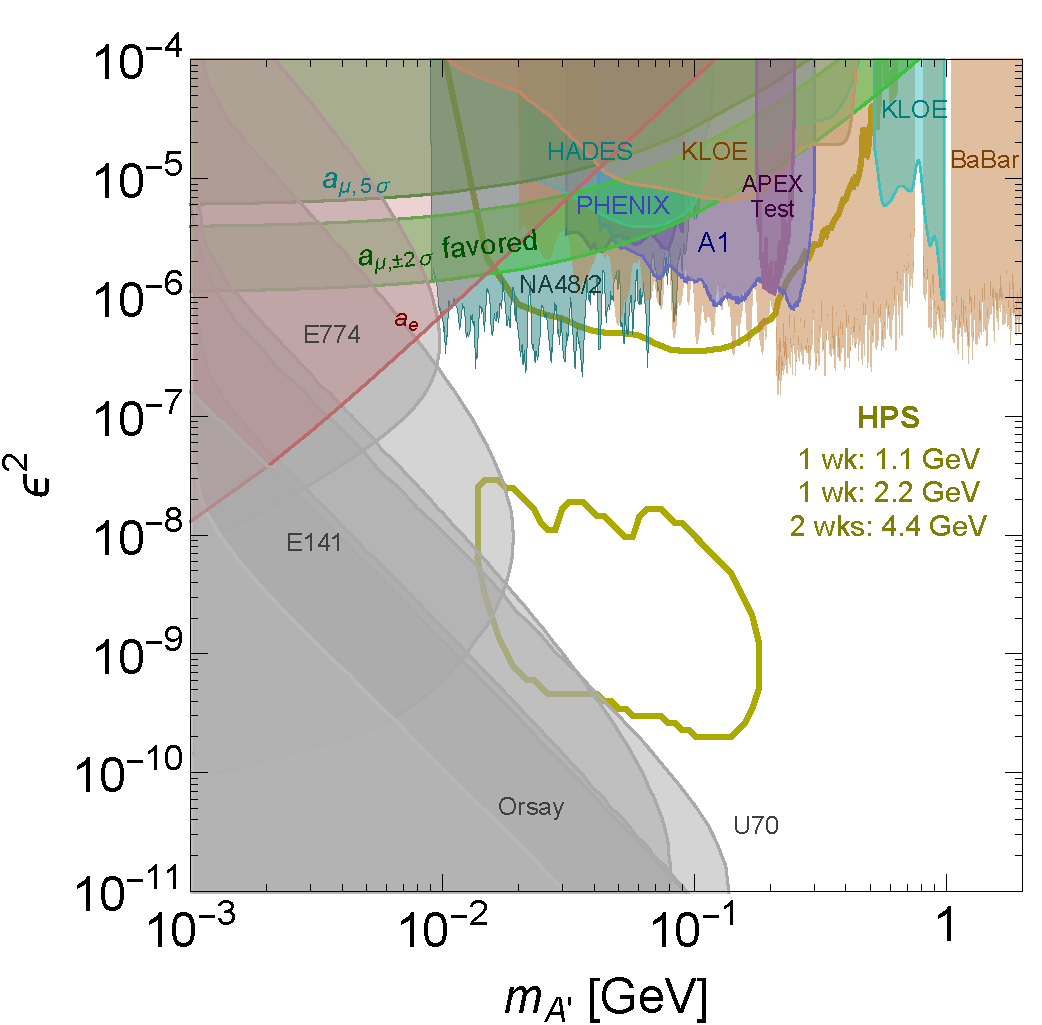
\includegraphics[width=\textwidth]{intro/figs/A-visible-HPS-official-6-2015}
    \caption{The yellow-green contours outline the expected reach (for exclusion at 90\% confidence level) for the HPS experiment with the run plan shown.
    The reach is split in two regions; the upper region corresponds to the bump-hunt and the lower region corresponds to the vertexing search.
    Existing limits from other experiments are plotted as shaded regions.
    The favored region from the muon $g-2$ anomaly is plotted as a shaded green band (upper left).}
    \label{fig:reach}
\end{figure}

If produced at HPS, heavy photons will decay to $e^+e^-$ pairs, possibly with some finite decay length; the HPS detector measures the momentum and decay vertex of the pairs.
The invariant mass and vertex of the pairs are used in two searches for heavy photons, covering different regions of the parameter space: a ``bump-hunt'' and a vertexing search.
The bump-hunt is a search for a narrow mass resonance above a smooth background, and is sensitive to heavy photons with relatively large couplings (and hence large production).
The vertexing search is a search for $e^+e^-$ pairs produced downstream of the target, and is sensitive to heavy photons with relatively small couplings (and hence long decay lengths).
This dissertation presents the vertexing search.

The 2015 HPS run was at a beam energy of 1.056 GeV, and nominal current of 50 nA.
The beam charge collected during physics data-taking is summarized in Figure \ref{fig:beamtime}.
Because detector commissioning was in progress throughout the run, the SVT was not moved to its nominal position (0.5 mm from the beam) until late in the run.
Roughly comparable amounts of data were recorded with the SVT at 1.5 mm and 0.5 mm from the beam.

This dissertation uses only the 2015 data from operation at 0.5 mm.
A total of 1166 nb$^{-1}$ of good data was recorded under these conditions, from May 13 through May 18.
This value is corrected for trigger deadtime and run quality, as described in Section \ref{sec:luminosity}; it is equivalent to 1.69 days of ideal running at the nominal beam current.
Approximately 90\% of the data was blinded so detector performance studies and analysis development could be done on the other 10\% without biasing the ultimate result.
This dissertation uses only the unblinded fraction, which is a total of 119 nb$^{-1}$ (0.172 days equivalent).

\begin{figure}[ht]
    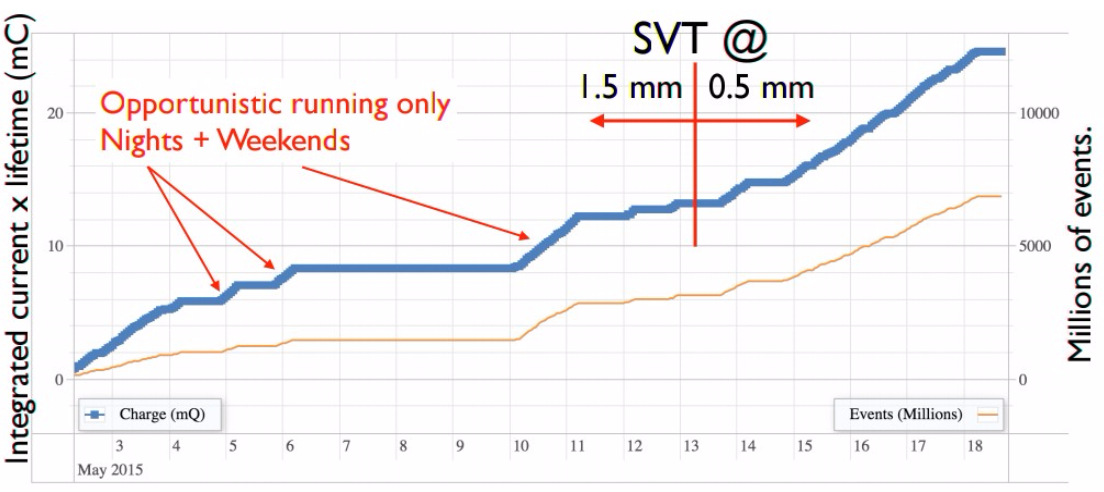
\includegraphics[width=\textwidth]{intro/figs/engrun-beamtime}
    \caption{Rough totals for integrated charge and event count during the 2015 HPS run. The numbers in this plot are not fully corrected for run and event quality.}
    \label{fig:beamtime}
\end{figure}

This dissertation presents the HPS experiment as a whole without specific reference to my personal contributions; those are summarized here.
I was responsible for the survey of the SVT, and assembled the modules and U-channels (both described in Section \ref{sec:svt_mechanical}).
I installed and documented the SVT cooling systems described in Section \ref{sec:svt_services}.
I developed the hit time reconstruction algorithm used in the SVT, described in Section \ref{sec:svt_hit_recon}.
I developed the detector readout and trigger simulations, which fully simulate the detector pileup, time evolution of pulses and readout pipelines, and trigger algorithms.
I used this trigger simulation for the performance studies and tuning of trigger parameters presented in the 2014 HPS proposal; the final trigger parameters described in Section \ref{sec:trigger_cuts} are based on that work.


Finally, I have had primary responsibility for the displaced-vertex search.
The analysis presented in Chapter \ref{sec:vertexing} was outlined in the 2014 HPS proposal \cite{collaboration_heavy_2013}, but I implemented it.
Section \ref{sec:proposal_reach} discusses differences between the proposal outline of the analysis, and what I have done.
\chapter{Motivation}
There is current theoretical and experimental interest in a massive $U(1)$ vector boson that does not couple directly to particles in the Standard Model, but gains a weak effective coupling to charged particles through kinetic mixing.
This particle is commonly called a heavy photon, dark photon, or $A'$, and is characterized by its mass $m_{A'}$ and a dimensionless coupling constant $\epsilon$.

The heavy photon is primarily motivated as part of a larger ``dark sector'' of particles that are not charged directly under the Standard Model forces.
Some sort of ``portal'' is necessary to create an interaction between the dark sector and the Standard Model.
The possible portals are restricted by the symmetries of the Standard Model, and the dominant candidates are commonly referred to as the vector, Higgs, neutrino, and axion portals; the heavy photon is the mediator for the vector portal \cite{essig_dark_2013}.
Dark sector particles are natural candidates for dark matter, and a heavy photon can be part of a mechanism that produces the observed dark matter abundance.

%Massive U(1) vector bosons, also known as heavy photons, are a natural consequence of many theories of physics beyond the Standard Model.
%Such a particle could kinetically mix with the photon, giving it an effective coupling to electric charge much smaller than the photon's direct coupling $\alpha$.
%A heavy photon is one of several ``portals'' by which a dark sector could interact with Standard Model matter.
%
%The existence of such a heavy photon is a possible explanation for the cosmic ray positron excess and the muon $g-2$ anomaly.

\section{Theory Summary}
The basic assumption behind the heavy photon is that there exists a second (broken) $U(1)$ symmetry, and that it interacts with Standard Model hypercharge via kinetic mixing \cite{holdom_two_1986}.
At low energies, this leads to the following gauge field Lagrangian, where $F_{\mu\nu}=\partial_\mu A_\nu - \partial_\nu A_\mu$ is the electromagnetic field strength, $F'_{\mu\nu} = \partial_\mu A'_\nu - \partial_\nu A'_\mu$ is the heavy photon field strength, and $\epsilon$ is the dimensionless coupling constant:

\begin{equation}
    \mathcal{L}_{\mathrm{gauge}}=-\frac{1}{4}F^{\mu\nu}F_{\mu\nu} - \frac{1}{4}F'^{\mu\nu}F'_{\mu\nu} + \frac{1}{2}\epsilon F^{\mu\nu}F'_{\mu\nu}
\end{equation}

The kinetic mixing means that the fields are not orthogonal.
Orthogonality can be restored by redefining the electromagnetic field according to $A^\mu \to A^\mu + \epsilon A'^\mu$.
This modifies the interaction Lagrangian as follows:

\begin{equation}
    A^\mu J^{EM}_\mu \to A^\mu J^{EM}_\mu + \epsilon A'^\mu J^{EM}_\mu 
\end{equation}

This implies that particles with electric charge acquire a coupling, proportional to $\epsilon$, to the heavy photon.
The converse is not true: hidden-sector particles with heavy photon couplings do not acquire couplings to the photon (such ``millicharged'' particles do occur if the new $U(1)$ is unbroken \cite{prinz_search_1998,davidson_updated_2000}) \cite{holdom_two_1986}.

If particles exist that are charged under both fields, kinetic mixing may arise from a one-loop diagram similar to Figure \ref{fig:oneloop}, with a natural scale of $\epsilon \sim 10^{-2}-10^{-4}$; on the other hand, GUT models require that one-loop contributions to $\epsilon$ vanish, and instead motivate two-loop contributions at $\epsilon \sim 10^{-3}-10^{-6}$ \cite{arkani-hamed_lhc_2008}.
Because kinetic mixing is a renormalizable interaction, $\epsilon$ is independent of the masses of the particles that give rise to it.
String theory models can motivate much smaller $\epsilon$, as low as $10^{-12}$ \cite{goodsell_naturally_2009,cicoli_testing_2011}.

\begin{figure}[ht]
    \begin{center}
        \begin{fmffile}{oneloop}
            \begin{fmfgraph*}(150,150)
                \fmfstraight 
                \fmfleft{i1}
                \fmfright{o1}
                \fmflabel{$\gamma$}{i1}
                \fmflabel{$A'$}{o1}
                \fmf{photon,tension=2}{i1,v1}
                \fmf{photon,tension=2}{v2,o1}
                \fmf{fermion,left}{v1,v2}
                \fmf{fermion,left}{v2,v1}
            \end{fmfgraph*}
        \end{fmffile}
    \end{center}
    \caption{One-loop diagram leading to kinetic mixing.}
    \label{fig:oneloop}
\end{figure}

There is a wide range of reasonable values for the mass $m_{A'}$.
Models where supersymmetry breaking is communicated by the kinetic mixing lead to natural mass scales of MeV-GeV \cite{baumgart_non-abelian_2009, morrissey_abelian_2009, cheung_kinetic_2009}.
String theory models typically tie the mass scale to $\epsilon$, and can motivate masses down to the meV scale \cite{goodsell_naturally_2009,cicoli_testing_2011}.

%If the new $U(1)$ is massless, the photon can be
%If the $A'$ is massless, the new $U(1)$ mixes 
%particles charged under the $A'$ gain a small electromagnetic charge. 
%
%Such millicharged particles have been the subject of direct experimental searches


%If the $A'$ is massive, particles charged under the $A'$ do not 
%
%massless U(1)': millicharge, paraphoton
%paraphoton doesn't couple to normal matter, para-matter gets millicharged
%
%massive U(1)': heavy photon
%photon doesn't couple to hidden sector, heavy photon couples to SM matter

\section{Observations Motivating a Heavy Photon}

\subsection{Dark Matter Annihilation}

Dark matter annihilation mediated by a heavy photon has been proposed as an explanation for several anomalies that have been reported in cosmic ray and X-ray observations.

The PAMELA satellite first observed that the positron fraction $\phi(e^+)/(\phi(e^+)+\phi(e^-))$ increases above 10 GeV.
This is inconsistent with the assumption that high-energy positrons originate in secondary production processes, from cosmic-ray nuclei interactions with interstellar gas.
Meanwhile, the antiproton fraction is consistent with secondary production.
Measurements by the Fermi Large Area Telescope and the Alpha Magnetic Spectrometer (AMS) confirmed the observation and extended it to higher energies \cite{the_fermi_lat_collaboration_measurement_2012,ams_collaboration_first_2013}.

The annihilation cross-section implied by the positron flux is large compared to the cross-section expected for a thermal relic, and also much larger than any observed annihilation to hadrons \cite{cholis_high_2009}.
This is consistent with annihilation to heavy photons with then decay to electrons and positrons, as shown in Figure \ref{fig:dm_annihilation} \cite{arkani-hamed_theory_2009}.
A heavy photon with $m_{A'}<2m_p$ cannot decay to $p\bar{p}$, and $m_{A'}$ in the MeV--GeV range (models with $m_{A'}$ in the 200--900 MeV range were tested in \cite{finkbeiner_consistent_2011}; if annihilation is dominated by local subhalos, lower mass ranges are allowed \cite{slatyer_sommerfeld-enhanced_2012}) creates Sommerfeld enhancement that boosts the annihilation cross-section at low velocities.

\begin{figure}[ht]
    \begin{center}
        \begin{fmffile}{annihilation}
            \begin{fmfgraph*}(150,150)
                \fmfstraight 
                \fmfleft{i1,i2}
                \fmfright{o0,o1,o2,o3,o4,o5}
                \fmflabel{$\chi$}{i1}
                \fmflabel{$\chi$}{i2}
                \fmflabel{$e^+$}{o1}
                \fmflabel{$e^-$}{o2}
                \fmflabel{$e^+$}{o3}
                \fmflabel{$e^-$}{o4}
                \fmf{fermion}{i1,v1,v2,i2}
                \fmf{photon,label=$A'$}{v1,v3}
                \fmf{photon,label=$A'$}{v2,v4}
                \fmf{fermion}{o1,v3,o2}
                \fmf{fermion}{o3,v4,o4}
            \end{fmfgraph*}
        \end{fmffile}
    \end{center}
    \caption{Dark matter annihilation through a heavy photon.}
    \label{fig:dm_annihilation}
\end{figure}

The positron fraction has more recently been disfavored as a motivation for the heavy photon.
A larger AMS data set shows the full shape of the positron spectrum is softer than would be expected from a heavy photon decaying directly to $e^+e^-$ \cite{ams_collaboration_high_2014}, but consistent with a pulsar origin for cosmic ray positrons \cite{cholis_dark_2013}.
Meanwhile, CMB observations put limits on the DM annihilation rate at recombination; measurements by Planck constrain the DM annihilation explanation for the positron fraction \cite{madhavacheril_current_2014}.
The positron spectrum may still be consistent with heavy photons decaying to intermediate states that then decay to $e^+e^-$ \cite{cholis_dark_2013}.

Gamma ray and X-ray excesses also motivate models of dark matter that include heavy photons.
Dark matter annihilation has been proposed as a source for an excess of high-energy gamma rays from the Galactic Center in Fermi data \cite{hooper_dark_2011}.
A 3.5 keV line seen in galaxy cluster X-ray spectra \cite{bulbul_detection_2014,boyarsky_unidentified_2014} has been suggested to come from collisional excitation and de-excitation of dark matter, in a model named eXciting Dark Matter (XDM) \cite{finkbeiner_x-ray_2014}.

\subsection{Halo Structure}
Observations of dark matter halos of galaxies and dwarf galaxies disagree with predictions based on the assumption of collisionless cold dark matter \cite{weinberg_cold_2013}.
These discrepancies have motivated models (``self-interacting dark matter,'' or SIDM) in which dark matter is self-interacting with a large but velocity-dependent cross-section, consistent with a heavy photon mediator.
This allows momentum diffusion in halos without disrupting high-velocity events such as the Bullet Cluster \cite{spergel_observational_2000,tulin_beyond_2013}.

Rotational velocities of observed Milky Way dwarf satellite galaxies are lower than the rotational velocities that simulations predict for the Milky Way's largest dark matter subhaloes.
This suggests that either the most massive dark matter subhalos fail to form dwarf galaxies, the massive subhalos do not exist, or the rotational velocities for a given subhalo mass are lower than predicted; this is known as the ``too big to fail'' problem \cite{boylan-kolchin_too_2011}.
Self-interacting dark matter reduces the central densities of subhalos and thus the rotational velocities \cite{vogelsberger_subhaloes_2012}.
Similarly, the observed density profiles of galaxies are better fit with a constant density core than the cuspy models from collisionless dark matter: this is the ``cusp-core'' problem \cite{de_naray_baryons_2011}
Both the observational evidence and the simulations continue to develop, and it may be possible to resolve the conflicts without abandoning collisionless dark matter \cite{oman_unexpected_2015,governato_cuspy_2012}.

\subsection{Light Dark Matter}

\subsection{Muon $g-2$}
\cite{2558}
\cite{1030}

\begin{figure}[ht]
    \begin{center}
        \begin{fmffile}{gm2}
            \begin{fmfgraph*}(150,150)
                \fmfstraight 
                \fmftop{o1}
                \fmfbottom{i1,i2}
                \fmflabel{$\mu$}{i1}
                \fmflabel{$\mu$}{i2}
                %\fmflabel{$e^+$}{o1}
                \fmf{fermion}{i1,v1,v2,v3,i2}
                \fmf{photon,label=$\gamma$}{v2,o1}
                \fmffreeze
                \fmf{photon,label=$A'$}{v1,v3}
            \end{fmfgraph*}
        \end{fmffile}
    \end{center}
    \caption{Heavy photon correction to the muon magnetic moment.}
    \label{fig:gm2}
\end{figure}

\begin{figure}[ht]
    \hspace{5mm}
    \begin{fmffile}{rad1}
        \begin{fmfgraph*}(150,150)
            \fmfstraight 
            \fmfleft{i1,i2,i3,i4}
            \fmfright{o1,o2,o3,o4}
            \fmflabel{$Z$}{i1}
            \fmflabel{$Z$}{o1}
            \fmflabel{$e^-$}{i3}
            \fmflabel{$e^-$}{o2}
            \fmflabel{$e^+$}{o3}
            \fmflabel{$e^-$}{o4}
            \fmf{fermion}{i3,v1,v3,o2}
            \fmf{heavy}{i1,v2,o1}
            \fmf{photon,tension=0,label=$\gamma$}{v1,v2}
            \fmf{fermion}{o3,v4,o4}
            \fmf{photon,tension=2,label=$\gamma$}{v3,v4}
        \end{fmfgraph*}
    \end{fmffile}
    \hspace{10mm}
    \begin{fmffile}{rad2}
        \begin{fmfgraph*}(150,150)
            \fmfstraight 
            \fmfleft{i1,i2,i3,i4}
            \fmfright{o1,o2,o3,o4}
            \fmflabel{$Z$}{i1}
            \fmflabel{$Z$}{o1}
            \fmflabel{$e^-$}{i3}
            \fmflabel{$e^-$}{o2}
            \fmflabel{$e^+$}{o3}
            \fmflabel{$e^-$}{o4}
            \fmf{fermion}{i3,v1,v3,o2}
            \fmf{heavy}{i1,v2,o1}
            \fmf{fermion}{o3,v4,o4}
            \fmf{photon,tension=2,label=$\gamma$}{v1,v4}
            \fmffreeze
            \fmf{photon,tension=0,label=$\gamma$}{v3,v2}
        \end{fmfgraph*}
    \end{fmffile}
    \hspace{5mm}
    \caption{Trident diagrams.}
    \label{fig:tridents_rad}
\end{figure}

\begin{figure}[ht]
    \hspace{5mm}
    \begin{fmffile}{bh1}
        \begin{fmfgraph*}(150,150)
            \fmfstraight 
            \fmfleft{i1,i2,i3,i4}
            \fmfright{o1,o2,o3,o4}
            \fmflabel{$Z$}{i1}
            \fmflabel{$Z$}{o1}
            \fmflabel{$e^-$}{i4}
            \fmflabel{$e^-$}{o2}
            \fmflabel{$e^+$}{o3}
            \fmflabel{$e^-$}{o4}
            \fmf{fermion}{i4,v1,o4}
            \fmf{heavy}{i1,v2,o1}
            \fmffreeze
            \fmf{photon,tension=1,label=$\gamma$}{v1,v3}
            \fmf{photon,tension=1,label=$\gamma$}{v2,v4}
            \fmf{fermion}{o2,v4,v3,o3}
        \end{fmfgraph*}
    \end{fmffile}
    \hspace{10mm}
    \begin{fmffile}{bh2}
        \begin{fmfgraph*}(150,150)
            \fmfstraight 
            \fmfleft{i1,i2,i3,i4}
            \fmfright{o1,o2,o3,o4}
            \fmflabel{$Z$}{i1}
            \fmflabel{$Z$}{o1}
            \fmflabel{$e^-$}{i4}
            \fmflabel{$e^-$}{o2}
            \fmflabel{$e^+$}{o3}
            \fmflabel{$e^-$}{o4}
            \fmf{fermion}{i4,v1,o4}
            \fmf{heavy}{i1,v2,o1}
            \fmffreeze
            \fmf{photon,tension=2,label=$\gamma$}{v1,v3}
            \fmf{photon,tension=2,label=$\gamma$}{v2,v4}
            \fmf{fermion}{o2,v3,v4,o3}
        \end{fmfgraph*}
    \end{fmffile}
    \hspace{5mm}
    \caption{Trident diagrams.}
    \label{fig:tridents_bh}
\end{figure}


\section{Signatures}

production cross-section

decay length

\section{Other Searches}


colliders

meson decays (LHCb)

positron on fixed target (VEPP)

old beam dumps

SeaQuest

\chapter{The HPS Detector}

The HPS detector is a spectrometer with a silicon vertex tracker (SVT) for momentum measurement and an electromagnetic calorimeter (ECal) for energy measurement and trigger.
The detector is installed in the middle dipole of a three-magnet chicane (see Figure \ref{fig:hps-pic}), with the field extending from the target to the end of the tracker.

The detector design is determined by physics needs.
To capture low-mass $A'$, the detector must have acceptance at small angles from the beam.
To get the best possible vertex resolution, the detector must operate as close to the target as possible.
Because multiple scattering dominates tracking resolution at HPS energies, the material in the tracking volume must be kept as low as possible.

Elastic scatters in the target send large numbers of electrons into the detector acceptance, so it needs to tolerate high rates and have a selective trigger.
Beam-gas interactions would create large detector backgrounds and fake $A'$ decays downstream of the target, so the beam must travel in vacuum all the way through HPS.
Bremsstrahlung energy losses in the target cause beam electrons to bend in the dipole field, forming a ``sheet of flame.'' To avoid this, no detector material is placed in the beam plane.

All parts of the HPS detector have the same minimum angle, or ``dead zone,'' at 15 milliradians.
This is set by the maximum rate tolerable in the first layer of the SVT: the occupancy within a resolution-limited hit time window must be less than 1\% for clean track reconstruction, and radiation damage must be kept low enough that the SVT remains fully functional after six months of operation.

\begin{figure}[htp]
    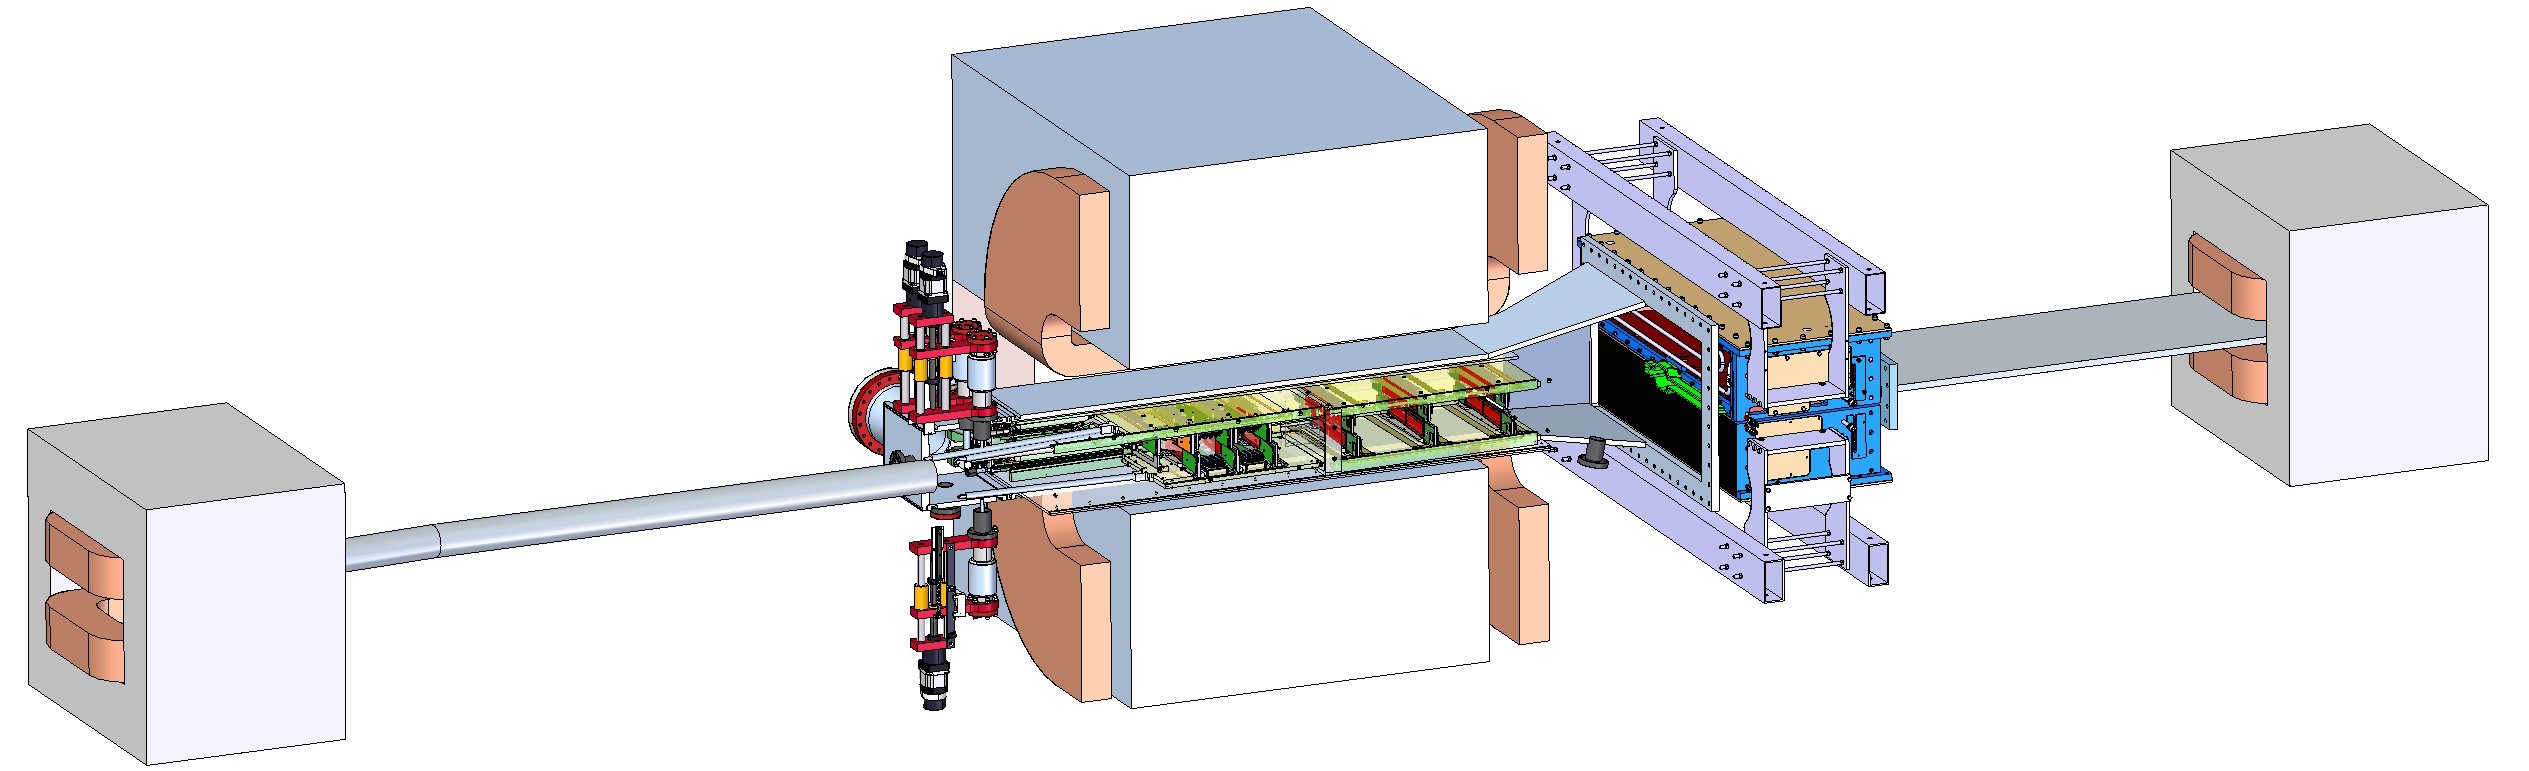
\includegraphics[width=\textwidth]{detector/figs/HPS-pic}
    \caption{View of the HPS setup.
    The beam direction is left to right.}
    \label{fig:hps-pic}
\end{figure}

\section{Beamline}
\label{sec:beamline}

HPS uses the CEBAF (Continuous Electron Beam Accelerator Facility) accelerator at Jefferson Lab (Figure \ref{fig:cebaf}).
CEBAF is a recirculating linac, where the electron beam can take multiple passes through the same set of accelerating cavities.
%CEBAF has a continuous duty cycle because it uses superconducting accelerating cavities, which can be operated continuously without 
The superconducting RF cavities used at CEBAF allow a continuous duty cycle, where beam bunches pass through the accelerator at 1500 MHz without interruption.
A system of RF separators delivers beam to each of four experimental halls at 250 or 500 MHz, and allows each hall to select its own beam energy.
HPS is installed in Hall B, the hall that typically operates at the lowest beam current.

The main detector in Hall B is CLAS (CEBAF Large-Acceptance Spectrometer), which is used for precision nuclear physics experiments with low-current (sub-$\mu$A) beams of electrons or photons. CEBAF recently underwent a major upgrade to increase the maximum beam energy from 6 GeV to 12 GeV, and add a new experimental hall (Hall D).
CLAS is undergoing a major rebuild (to become the CLAS12 detector) for 12 GeV operation, and this work is still in progress.
The 2015 and 2016 HPS runs were conducted after CEBAF began 12 GeV operations but before much of CLAS12 was complete; HPS is the first Hall B experiment of the 12 GeV era, albeit not operating at 12 GeV (the maximum field of the HPS magnets limits HPS to 6.6 GeV beam).

The injector energy is 100 MeV and one pass through the linacs adds 2.2 GeV to the beam energy, so in normal operation, the available beam energies at Hall B are 100 MeV + $n*2.2$ GeV where $n$ is 1 through 5.
During the 2015 engineering run, a mechanical problem disabled one of the two CEBAF helium liquifiers.
With half the cooling power, the superconducting cavities could only be run at half the nominal gradient.
HPS took the opportunity to run at 1.056 GeV, an energy that is not normally available.

HPS relies on the continuous beam structure at CEBAF to reduce pileup.
A beam bunch arrives at HPS every 2 ns, which is comparable to the time resolution of the detectors.
This means that beam backgrounds are spread in time as uniformly as possible.
A larger bunch spacing or lower duty cycle would increase the amount of beam background that overlaps an event of interest.

\begin{figure}[htp]
    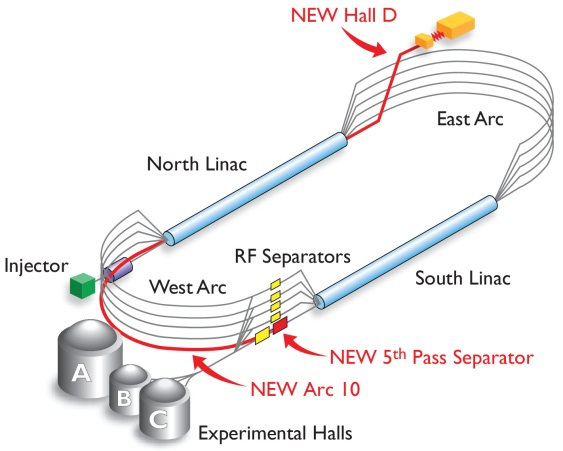
\includegraphics[width=0.6\textwidth]{detector/figs/cebaf}
    \caption{Schematic of the CEBAF accelerator, highlighting components added for the 12 GeV upgrade.}
    \label{fig:cebaf}
\end{figure}

\subsection{Hall B Beamline and Instrumentation}

\begin{figure}[htp]
    \begin{center}
        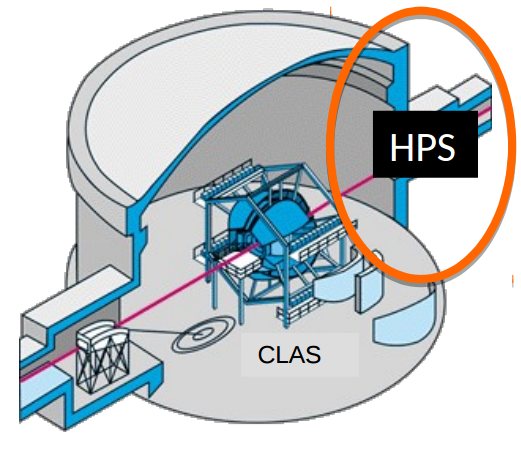
\includegraphics[width=0.5\textwidth]{detector/figs/hallb}
    \end{center}
    \caption{Location of the HPS setup, in the downstream alcove of Hall B.
    The beam direction is left to right.}
    \label{fig:hallb}
\end{figure}

HPS is installed in the downstream alcove of Hall B: see Figure \ref{fig:hallb}.
Since CLAS12 construction is in progress, a plain beam pipe was installed to pass the beam through CLAS, and HPS operations were limited to nights and weekends to allow CLAS construction to continue.

The Hall B beamline can be configured for delivery of both electron and photon beams.
Soon after it enters the hall, the CEBAF electron beam passes through a large ``tagger'' magnet.
If a target is positioned upstream of the tagger magnet, a beam of bremsstrahlung photons can be sent to experiments while the tagger magnet sends the beam to a dump (the ``tagger dump'') and the bremsstrahlung electrons to wire chambers (``tagging'' the energy of each photon).
For HPS operation the beamline is run in the electron configuration (tagger magnet de-energized, electrons to HPS and main dump), but the photon configuration (tagger magnet energized, electrons to tagger dump) is still used for beam setup since it allows for tuning the upstream part of the beamline without disrupting the beam at HPS.

The Hall B beam instrumentation consists of beam position monitors (BPMs), halo monitors, wire scanners, viewers, and a Faraday cup.

BPMs detect the current induced by passing beam bunches in order to measure the current and/or position of the beam.
Since this is a noncontact measurement, BPMs operate continuously during operations and provide a record of beam changes during data taking.

Halo monitors are small particle detectors (mostly scintillators) positioned around the beam pipe.
If the beam is obstructed, defocused or missteered, it will scatter into the halo monitors.
%The halo monitors can be used as part of the fast shut down (FSD) system.

Wire scanners consist of a set of wires mounted on a motorized frame.
The beam position and size is measured by scanning the wires across the beam; the halo counter rates increase in proportion to the amount of beam subtended by a wire.
An example wire scan is shown in Figure \ref{fig:beamsize}.
All harps have at least one vertical and one horizontal wire; some have a diagonal ($45^\circ$) wire for measuring the beam tilt and/or thicker wires for measuring the tails of the beam.

\begin{figure}[htp]
    \begin{center}
        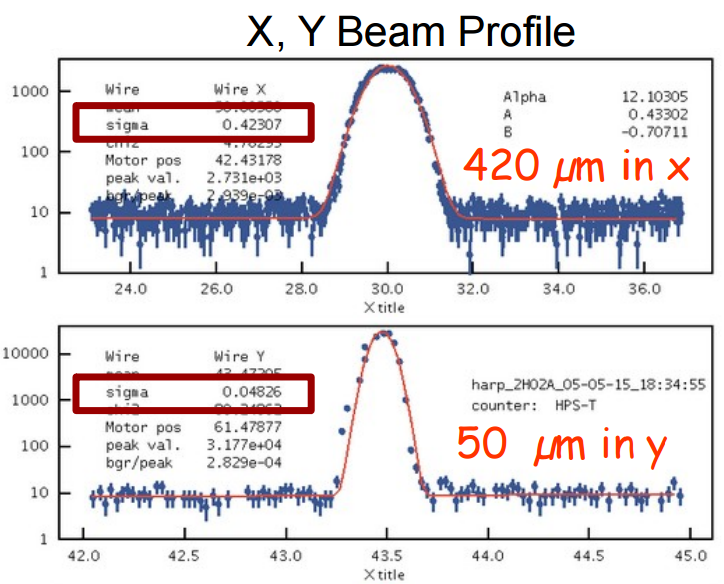
\includegraphics[width=0.5\textwidth]{detector/figs/beamsize}
    \end{center}
    \caption{A representative wire scan measurement of the beam size.
    This wire scan was taken early in the 2015 run; the beam size in X was reduced later in the run, and all physics data was recorded with a beam size of roughly $150\times 50$ $\mu$m.
    }
    \label{fig:beamsize}
\end{figure}

Beam viewers consist of a thin screen that emits light when the beam passes through it, and a video camera for viewing the shape and position of the beam.
Fluorescent screens are sensitive but are susceptible to saturation and blooming effects, and are most useful for viewing the beam position.
A screen using optical transition radiation (OTR) is dimmer, but does not saturate and accurately shows the beam shape.
One fluorescent screen is mounted in front of the Hall B tagger dump.
Two fluorescent screens of different types, and one OTR screen, are mounted on a motorized carousel in front of the Hall B main dump.

The Hall B beamline terminates in a Faraday cup, which directly measures the beam charge.
This is the most accurate measurement of the beam current.

\subsection{Beam Quality and Protection}
HPS has two primary concerns regarding the beam.
First, since the SVT is so close to the beam, the SVT must be protected both from beam being directed into the silicon and causing damage, and from stray beam electrons hitting the inner regions of the active silicon and adding to the detector pileup.
This implies strong beam protection controls and low beam halo.
Second, a small beam spot is important for event quality cuts; if the beam spot is small (ideally, smaller than detector resolution), poorly reconstructed tracks or vertices that are not consistent with an origin at the beam spot can be rejected.
%Beyond a small beam spot, this implies a stable beam, since beam motion will smear the effective beam spot size, and a repeatable beam position from run to run.

Active beam protection is provided by the CEBAF fast shutdown (FSD) system.
The FSD system is an interlock which, when triggered, shuts off the electron gun in the injector.
In addition to the large amount of beam instrumentation that is normally connected to the FSD, the set of halo counters closest to HPS were used to provide an FSD signal.
This halo counter FSD was configured so that an abnormally high rate on the halo counters (the threshold being set as low as possible without causing spurious beam trips) would trip the beam in 1 ms.
If the beam were to move into the SVT sensors, it would hit the inactive edge of the silicon (0.5 mm from the nominal beam position) first.
The beam scattering from the silicon would trip the halo counter FSD, hopefully before the beam could reach the active silicon (1.5 mm from the nominal beam position).

A collimator provides passive beam protection.
The collimator is a tungsten plate 1 cm thick with machined slots of different widths, mounted on a linear shift so the appropriate slot can be selected and positioned precisely.
For the 2015 run, the 3 mm slot was used; this slot width is equal to the gap between the active regions of the SVT.
If the beam were to move into active silicon, the collimator would absorb and spread the beam enough that the silicon would not be damaged in the time it would take for the FSD to stop the beam.
%beam protection, FSD

Measurements of the beam halo, such as shown in Figure \ref{fig:beam-tails}, show that the beam profile does not deviate from a Gaussian for five orders of magnitude; the rate of beam electrons outside of $\pm 0.5$ mm is $10^{-5}$ of the beam current.
At this level, the rate of beam halo electrons hitting the innermost strips of the SVT is less than the rate of scattered electrons from the target.

\begin{figure}[htp]
    \begin{center}
        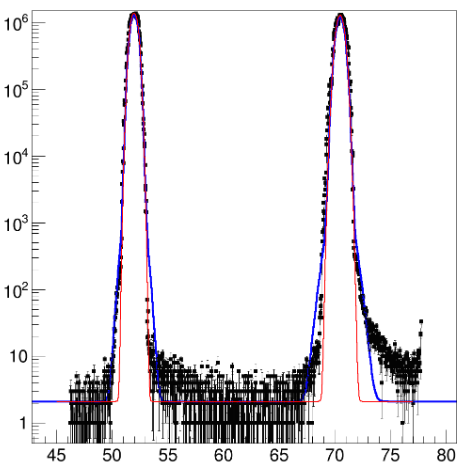
\includegraphics[width=0.5\textwidth]{detector/figs/beam-tails}
    \end{center}
    \caption{A wire scan measurement of the beam halo.
    The black data points show the halo counter rates as a function of motor position.
    The two peaks correspond to the horizontal and vertical wires (each wire is iron, 1 mm diameter) crossing the beam.
    The red curve is a fit to the Gaussian core of the beam, and the blue curve is its convolution with the wire size.
    The data is consistent with the fits over five orders of magnitude, indicating that the beam halo is of that level.
    }
    \label{fig:beam-tails}
\end{figure}

HPS requested a beam size that was smaller in X than in Y.
Since the vertex resolution is better in Y ($\sim 150$ $\mu$m) than in X ($\sim 300$ $\mu$m), and target heating was believed to limit the minimum safe beam size, the desired beam shape was narrow ($\sim 50$ $\mu$m) in Y and wider ($\sim 300$ $\mu$m) in X.
One challenge in making such an asymmetric beamspot is that the beam tilt must be precisely controlled.
As shown in Figure \ref{fig:beamsize}, this was achieved.
It was later realized that target heating was not a serious concern, and all 2015 physics data was recorded with a beam size of $\sim 50$ $\mu$m in Y and $\sim 150$ $\mu$m in X.

\subsection{HPS Beamline Elements}

The HPS chicane, shown in Figure \ref{fig:hps-pic}, consists of three dipoles with fields in the vertical direction.
The three magnets of the chicane are repurposed from a past Hall B experiment.
The detector is installed in the central magnet (the ``pair spectrometer'' magnet), which is a 18D36 magnet (pole length 91.44 cm, width 45.72 cm), and was operated at a field strength of 0.24 T for the 2015 run.
The outer magnets are identical ``Frascati''-type magnets, equidistant from the analyzing magnet and operated at equal field strengths, such that the $\int B dl$ of each Frascati magnet is half that of the analyzing magnet (and opposite in sign).
This ensures that the beam trajectory downstream of the chicane is the same whether or not the chicane is energized.

A series of connected vacuum chambers constitute the HPS beam path.
A short rectangular chamber upstream of the pair spectrometer magnet provides feedthroughs for SVT services (motion, cooling, power, data), further described in Section \ref{sec:svt_services}.
A long rectangular chamber (inherited with the pair spectrometer magnet) fills the magnet bore and extends downstream; the downstream segment flares outward to allow charged particles to bend.
The next chamber (shown in Figure \ref{fig:ecal_chamber}) closes off the vacuum chamber, except for a slot-shaped channel that allows the beam and the sheet of flame to pass through to the dump; the ECal (which does not operate in vacuum) closely surrounds the slot on top and bottom.

\begin{figure}[htp]
    \begin{center}
        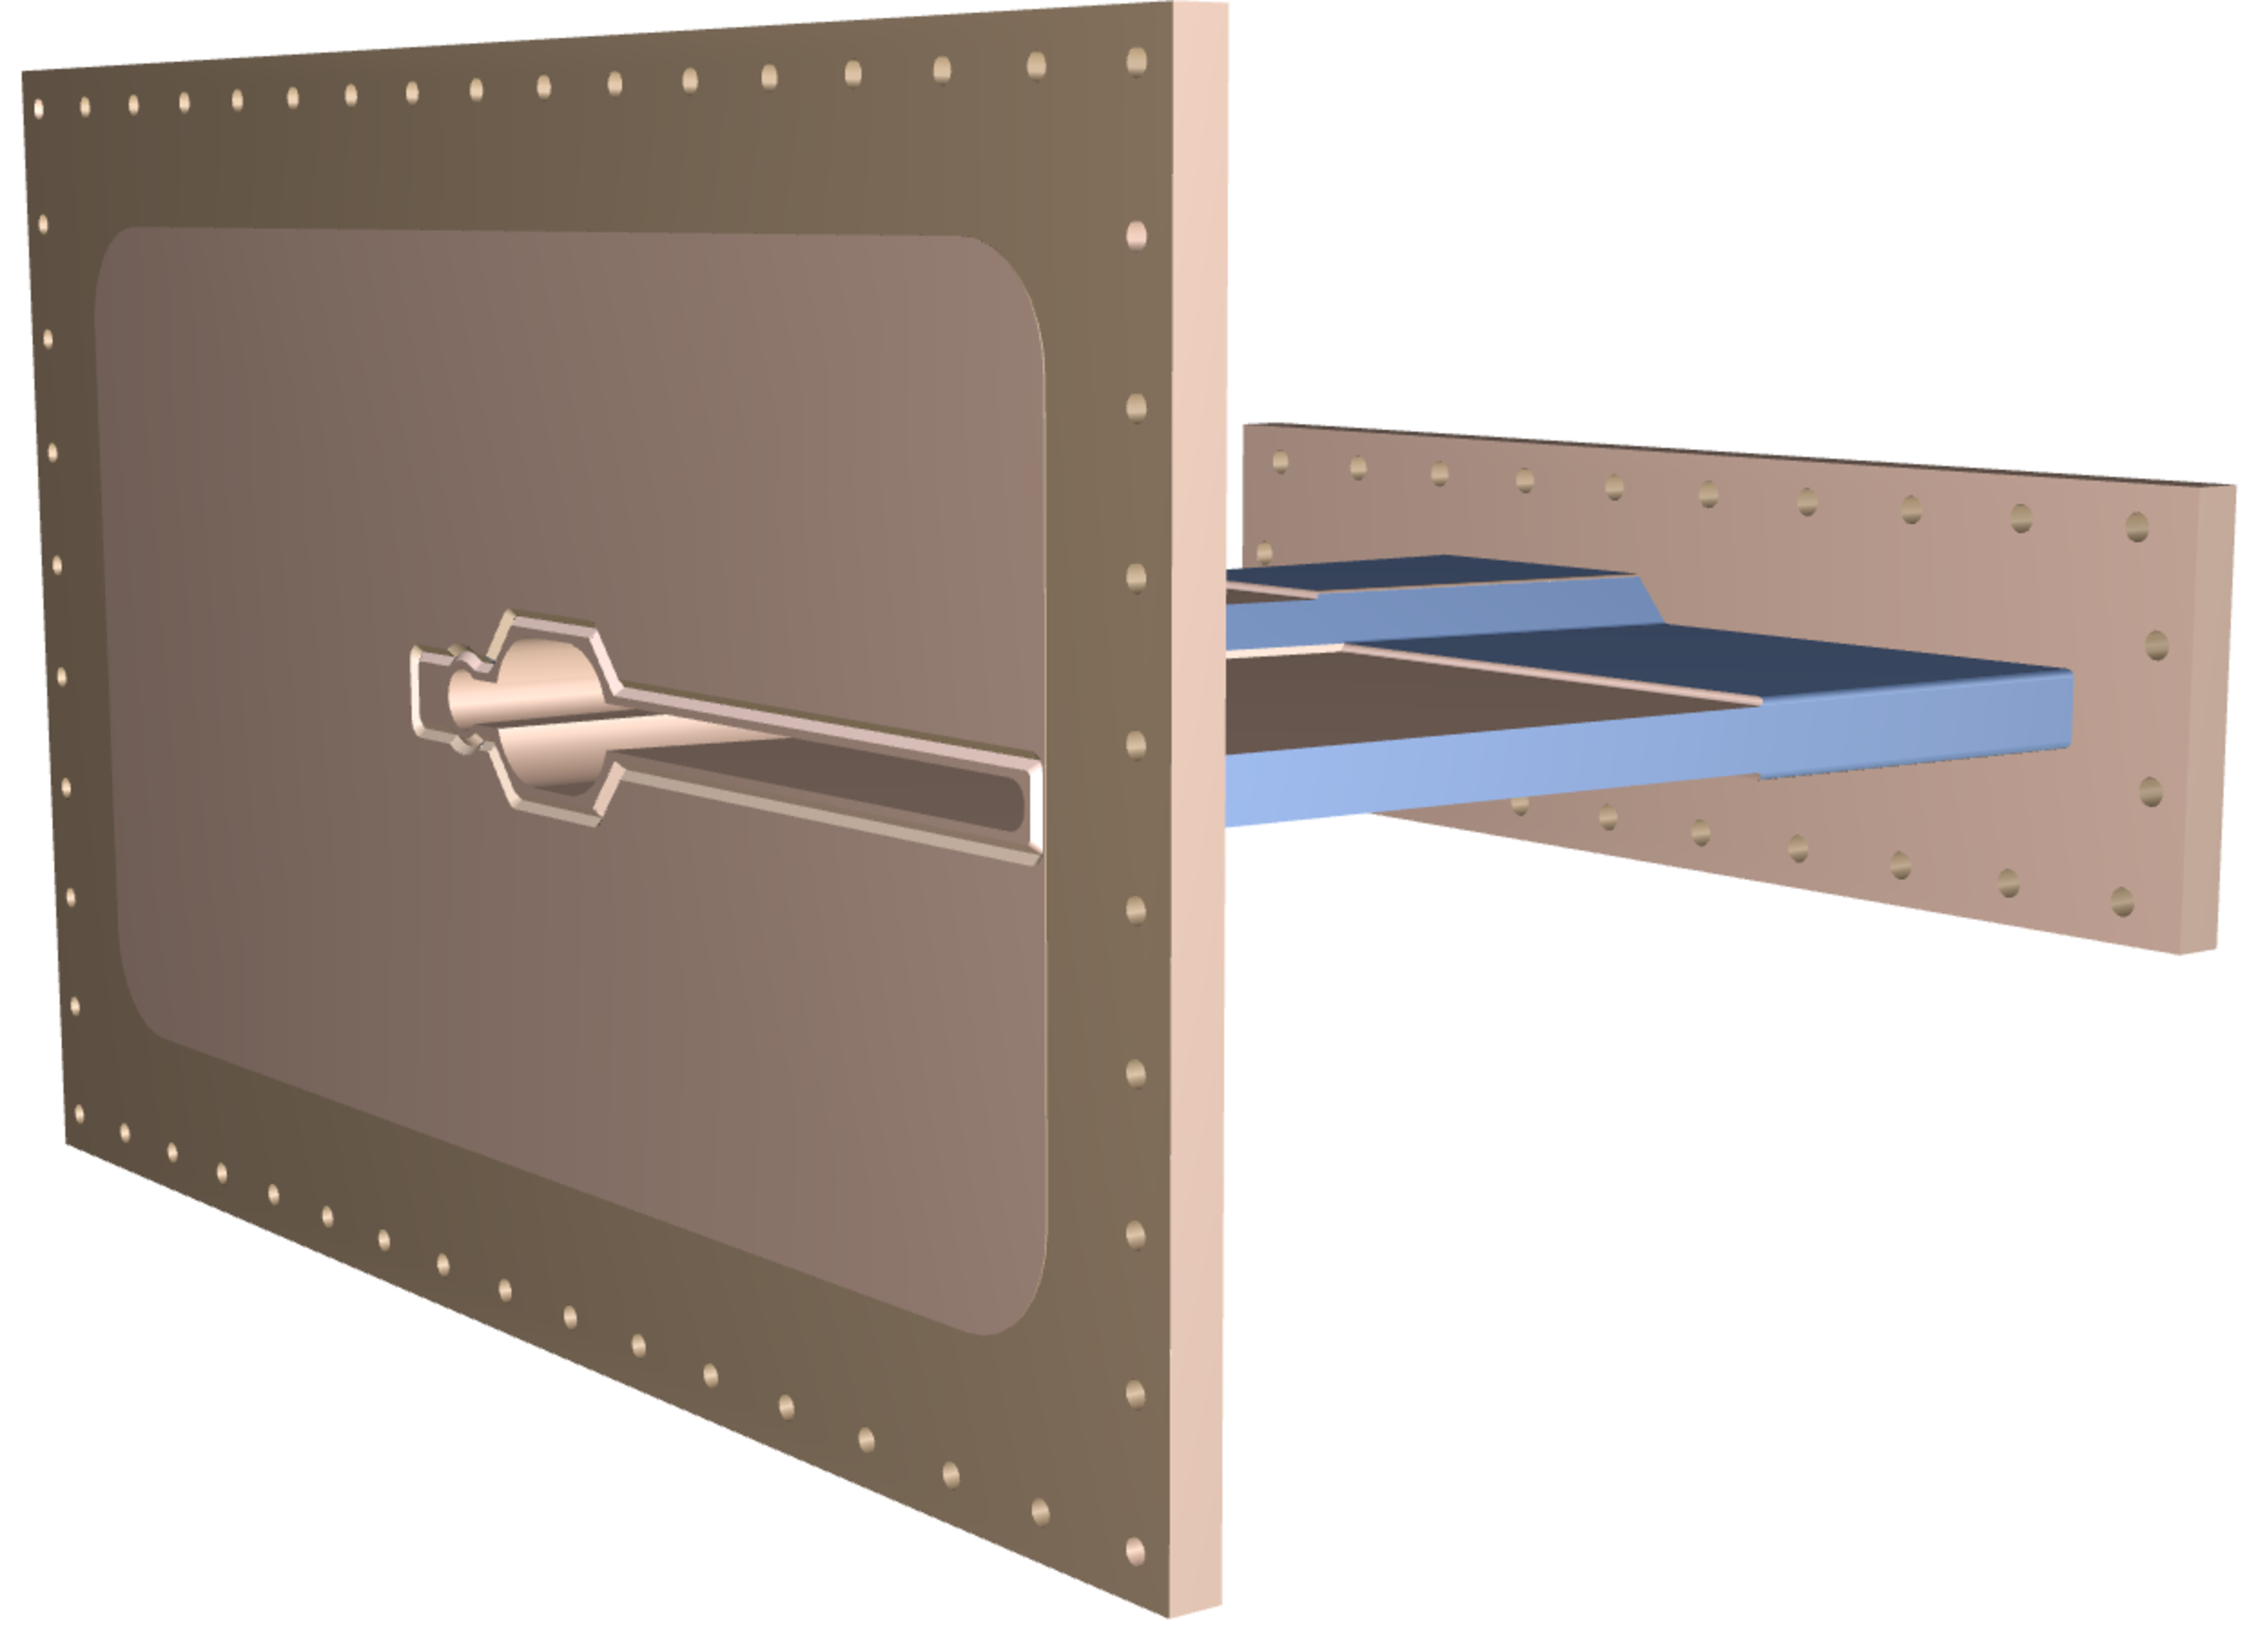
\includegraphics[width=0.5\textwidth]{detector/figs/ecal_vac}
    \end{center}
    \caption{A rendering of the ECal vacuum chamber.
    The large rectangular flange closes off the pair spectrometer vacuum chamber.
    The slot has a complex shape to pass different types of particles radiating from the target.
    From left to right: the round tube passes bremsstrahlung photons, the oval tube passes the beam (which is enlarged by small-angle scattering) and M{\o}ller-scattered electrons, and the wide slot passes bremsstrahlung electrons.
    The walls of the slot are quite thin and a strut of aluminum honeycomb (not visible) supports it against air pressure.
    }
    \label{fig:ecal_chamber}
\end{figure}

The HPS target is a set of foils mounted on a common frame.
There are two tungsten foils, one graphite foil, and one polyethylene foil.
The tungsten foils have design thicknesses of 0.125\% and 0.25\% radiation lengths (as-built thicknesses are 0.116\% and 0.223\%); the 0.125\% $X_0$ foil is for runs at 1.1 and 2.2 GeV, and the 0.25\% $X_0$ foil is for runs at 4.4 and 6.6 GeV.
A linear shift moves the frame up and down so the foils can be moved in and out of the beam; since the target needs to be at the face of the magnet, and the linear shift is on one of the flanges of the upstream vacuum chamber, the target frame is cantilevered on a ceramic support rod.

\begin{figure}[htp]
    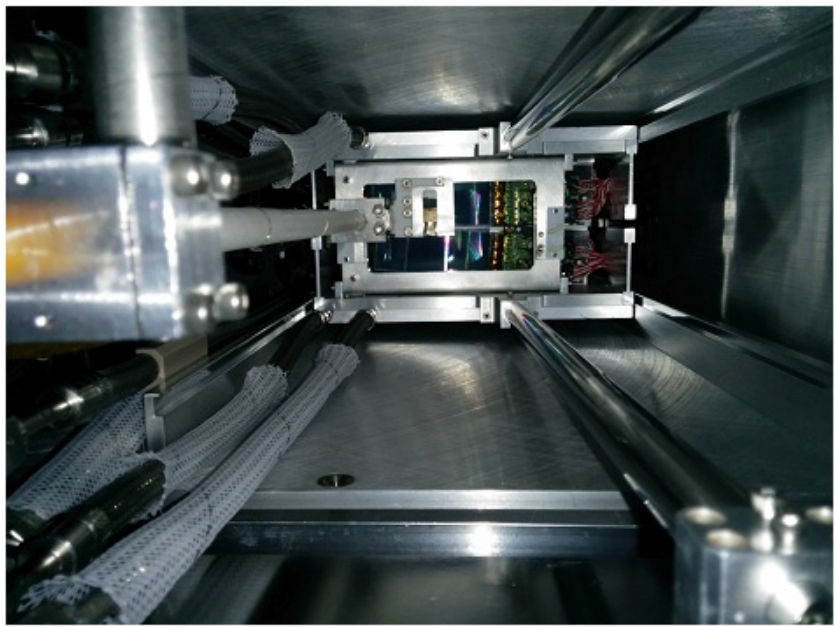
\includegraphics[width=\textwidth]{detector/figs/target_photo}
    \caption{Beam's-eye view of the HPS target and the front of the SVT after installation.
    The vertical rod from the target linear shift (foreground left), the ceramic support rod, and the target frame (center, offset to the right from the end of the support rod) are visible.
    }
    \label{fig:target_photo}
\end{figure}

\section{Silicon Vertex Tracker}

\begin{figure}[htp]
    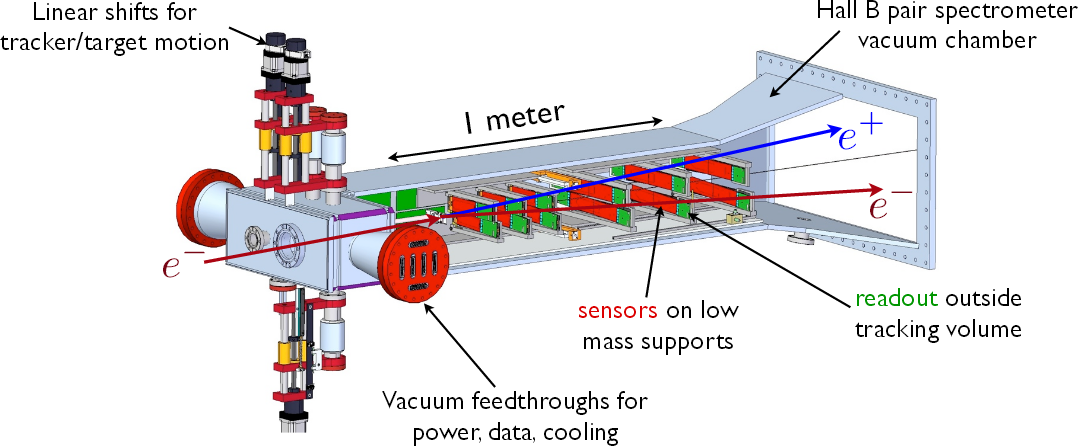
\includegraphics[width=\textwidth]{detector/figs/svt_cutaway}
    \caption{Schematic of the SVT and its support systems.}
    \label{fig:svt-schematic}
\end{figure}

\begin{figure}[htp]
    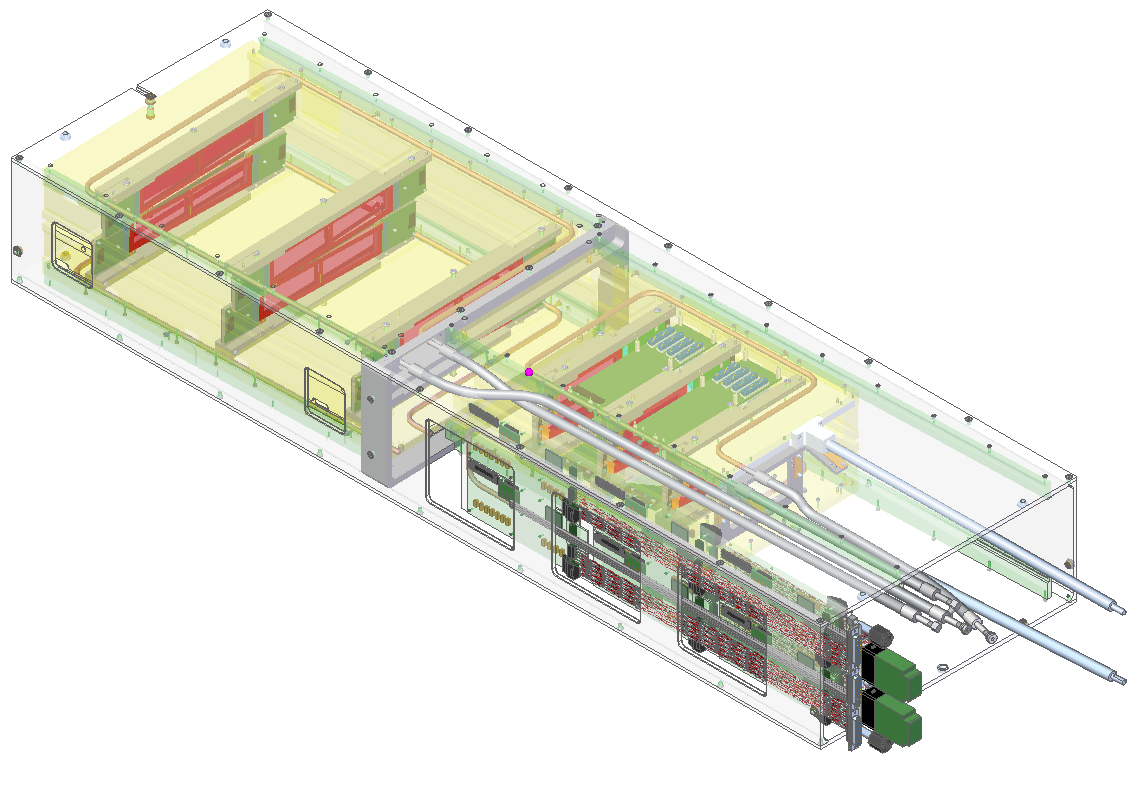
\includegraphics[width=\textwidth]{detector/figs/svt_drawing}
    \caption{Rendering of the SVT as built, showing cooling lines and motion levers.}
    \label{fig:svt-drawing}
\end{figure}

The silicon vertex tracker (SVT) measures track momentum and vertex position.

HPS uses silicon microstrips because they provide good time resolution, low mass, and high rate.
Because a microstrip sensor can only make a 1-D measurement (it identifies the strip that was hit, but not the hit position along the strip), each measurement station (called a ``layer'') uses two sensors at an angle relative to each other.
For HPS this stereo angle is kept small, so all sensors have their strips pointing roughly in the bend direction.
A small stereo angle is a compromise: it sacrifices measurement resolution in the strip direction, but it is less likely that two particles will create ``ghost hits'' when the strips they hit intersect each other.
The stereo angle is not uniform throughout the SVT (it is 100 milliradians in the upstream half, 50 milliradians in the downstream half), which prevents ghost hits from creating ghost tracks.

The SVT is made of six layers at different distances from the target: this number allows for 5-hit tracking even if a particle misses one layer.
Layer 1 is 10 cm from the target; this is the closest we can safely operate while allowing 500 $\mu$m distance from the beam to the edge of the sensors, which have a 1 mm border of inactive silicon.
Layer 6 is 90 cm from the target, just at the end of the uniform field region of the analyzing magnet; maximizing the length of the tracker maximizes the momentum resolution.
Layers 1--3 use single sensors; layers 4--6, where tracks have bent out to the sides, use two sensors joined end to end.
The layout of the six layers is summarized in Table \ref{tab:svt_layout}.

\begin{table}[htp]
    \begin{center}
        \caption{Layout of the HPS SVT.  The angle of stereo sensors is relative to the bend plane.}
        \begin{tabular}{lcccccc}   
            \hline \hline 
            Layer number & 1 & 2 & 3 & 4 & 5 & 6 \\      
            \hline
            nominal $z$, from target (cm)  & 10 & 20 & 30 & 50 & 70  & 90 \\ 
            Stereo Angle (mrad)  & 100 & 100 & 100 & 50 & 50 & 50 \\ 
            Bend-plane resolution ($\mu m$)  & $\approx$60 & $\approx$60 & $\approx$60 & $\approx$120 & $\approx$120 & $\approx$120 \\ 
            Non-bend resolution ($\mu m$)  & $\approx$6 & $\approx$6 & $\approx$6 & $\approx$6 & $\approx$6  & $\approx$6 \\ 
            Number of sensors  & 4 & 4 & 4 & 8 & 8 & 8 \\ 
            Nominal dead zone in $y$ (mm)  & $\pm1.5$  & $\pm3.0$  & $\pm4.5$  & $\pm7.5$  & $\pm10.5$ & $\pm13.5$  \\ 
            Module power consumption (W) & 6.9 & 6.9 & 6.9 & 13.8 & 13.8 & 13.8 \\
            \hline \hline
        \end{tabular}
        \label{tab:svt_layout} 
    \end{center}
\end{table}

Because the SVT operates in a high magnetic field and in vacuum, materials must be compatible.
All materials are checked for vacuum compatibility by pumping test samples to high vacuum in a test chamber.
Only nonmagnetic materials are used; inductors used on the frontend boards are air-core (instead of ferrite, which would saturate).

\subsection{Sensors and Readout}
HPS uses silicon microstrip sensors that were originally produced for the run IIb upgrade of the D{\O} detector at Fermilab.
This upgrade would have replaced the entire SMT (silicon microstrip tracker).
The full SMT upgrade was cancelled in favor of an insertable Layer 0, but not before sensors had already been procured.
The sensors used for HPS are those that would have been used for layers 2--5 of the new D{\O} tracker.

The HPS sensors are single-sided p+n with AC-coupled readout: the bulk is lightly doped n-type silicon with $<$100$>$ crystal orientation, and the strip implants are strongly p-type doped.
The strips are biased through polysilicon resistors at the ends of the strips, and capacitively coupled to aluminum readout strips that run on top of the strips.
Only every other strip is read out; the ``readout'' strips capacitively couple to the intermediate ``sense'' strips, so a hit in a sense strip splits its charge between the neighboring readout strips.

Radiation damage limits the useful lifetime of silicon sensors.
Incident particles can displace silicon atoms from their places in the crystal lattice, which effectively converts the n-type bulk of the sensor to p-type (type inversion).
This increases the depletion voltage, so the sensor bias must be increased to keep the same charge collection efficiency; the sensor lifetime is therefore limited by the breakdown voltage of the sensor.
The defects also increase the leakage current, which leads to increased sensor heating.
The HPS sensors are specified to have a breakdown voltage of greater than 350 V, and a further selection was made to only use sensors with a breakdown voltage in excess of 1000 V.

\begin{table}[htp]
    \begin{center}
        \caption{Specifications of the SVT sensors.
        Breakdown voltage specification is value accepted for use in HPS; procurement specification was looser.}
        \begin{tabular}{lc}   
            \hline \hline
            Thickness & 320 $\mu$m \\
            Overall area (L$\times$W) & 100 mm $\times$ 40.34 mm\\
            Active area (L$\times$W) & 98.33 mm $\times$ 38.34 mm\\
            Strip pitch (count) & 30 $\mu$m (1277)\\
            Readout pitch (count) & 60 $\mu$m (639)\\
            Depletion voltage & 110-130 V (typical)\\
            Breakdown voltage & $>$1000 V\\
            \hline \hline
        \end{tabular}
        \label{tab:sensor_spec} 
    \end{center}
\end{table}

The sensors are read out by the APV25 readout chip \cite{french_design_2001}.
This chip was developed for silicon microstrip readout in the CMS tracker.
Because the APV25 can read out multiple consecutive samples of its shaper waveform, it can be used for pileup rejection and high-precision hit time reconstruction.
This is an essential feature for HPS and other experiments (notably the Belle II SVD \cite{liu_belle_2012}) with CW beam and high pileup.

Each APV25 chip has 128 input channels.
One channel consists of a charge-sensitive preamp with an optional inverter, CR-RC shaper, and 192-cell analog pipeline.
We run the chip with a 24 ns clock: the design clock period is 25 ns to match the LHC bunch crossing period, but 24 ns is an even multiple of the standard JLab clock.
On each clock, each channel samples its shaper output and stores it in a cell of its pipeline.
On a trigger, each channel reads out the appropriate pipeline cell, and the chip multiplexes the 128 signals onto a single differential current output.

\begin{figure}[htp]
    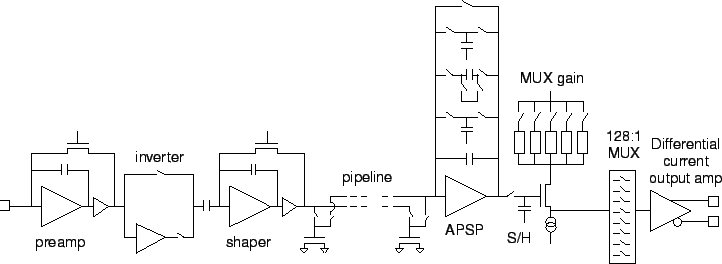
\includegraphics[width=\textwidth]{detector/figs/apv25}
    \caption{Schematic of the APV25. The APSP (analog pulse shape processor) is disabled in the ``multi-peak'' readout mode used by HPS.}
    \label{fig:apv25}
\end{figure}

HPS runs the APV25 in its ``multi-peak'' readout mode, which allows us to read out six consecutive pipeline cells for each trigger.
Six samples per trigger, combined with knowledge of the shaper pulse shape (from an offline calibration), allows us to fit the shaper output to the sum of one or two pulses.
The result is a reconstructed hit time and amplitude that is unaffected by a pileup hit that comes before or after the hit of interest.

\subsection{Mechanical Support}
\label{sec:svt_mechanical}

The base unit of the SVT is a ``half-module'' comprising a low-mass support structure, sensors, and hybrid readout circuit boards.
Half-modules are the only unit of the SVT that cannot be disassembled and reworked.
Two types of half-modules are used: layers 1--3 use single-ended half-modules with one sensor and hybrid each, and layers 4--6 use double-ended half-modules with two sensors and hybrids each.
A single half-module provides a single measurement (axial or stereo) for one half (top or bottom) of a layer.

\begin{figure}[htp]
    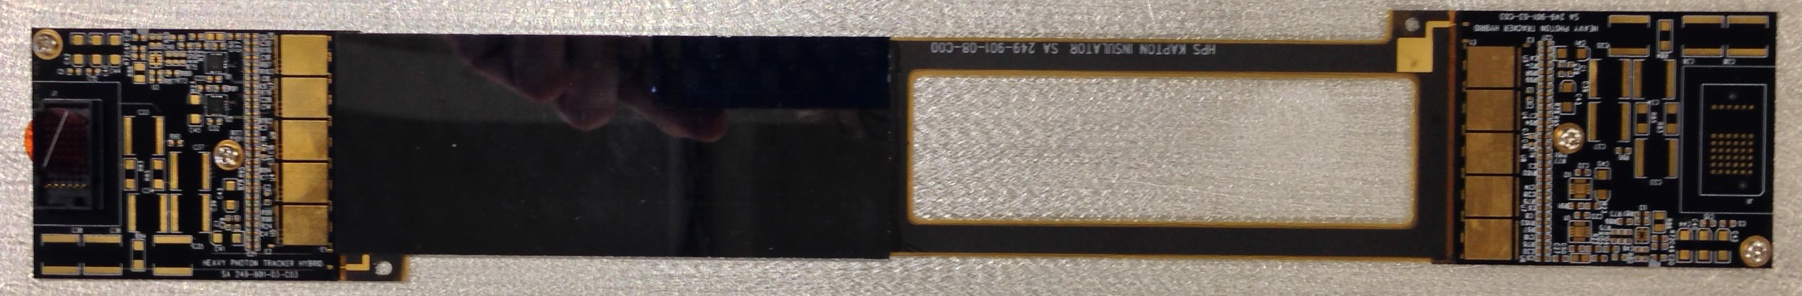
\includegraphics[width=\textwidth]{detector/figs/l456_hm}
    \caption{One half-module for L4--6. The two hybrids (without readout chips, which would be mounted on the gold pads) are at the left and right ends. One sensor is in place, on the left. The carbon fiber support and Kapton passivation layer are visible on the right.}
    \label{fig:l456_hm}
\end{figure}

The hybrid circuit board carries the APV25 readout chips, and connects the sensor to the rest of the DAQ.
The input channels of the APV25 chips are wirebonded directly to the sensor; the APV25 power, output channels, and control lines are wirebonded to the hybrid.
The hybrid also carries filter capacitors for the sensor bias, and temperature sensors to monitor the sensor temperature.

The carbon fiber support structure provides structural support for the silicon, and acts as a ground plane for the half-module.
A layer of Kapton insulation isolates the carbon fiber from the back surface of the sensor, which is held at high voltage.
The carbon fiber and Kapton are thinner than the silicon and contribute negligibly to the material seen by particles; cutouts further reduce any effect.
The sensors and hybrids are glued to the support structure with epoxy.

Two half-modules are paired back-to-back to form a ``module.''
The axial half-module is oriented with its strips pointing in the bend direction; the stereo half-module is rotated so it dips into the beam plane on the positron side (where beam backgrounds are less intense).
The modules are assembled using pairing fixtures, which are machined to set the edges of the sensors at precisely the correct height and angle.

\begin{figure}[htp]
    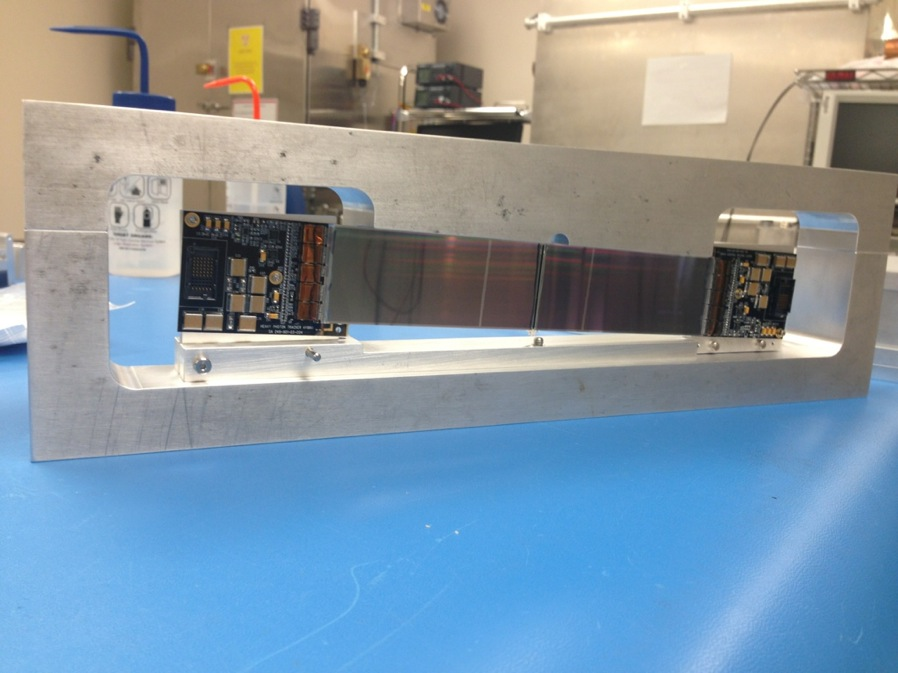
\includegraphics[width=\textwidth]{detector/figs/pairing_l456}
    \caption{The L4--6 pairing fixture, with one half-module in place.}
    \label{fig:l456_pairing}
\end{figure}

The aluminum module support holds the half-modules at both ends.
Heat generated by the hybrids is pulled out through the module support, which is in close thermal contact with the APV25 chips and the sensors through parallel paths so that the sensors can be kept colder than the APV25 chips.
The module support and the half-modules contract at different rates when the SVT is cooled to its operating temperature, so the module support must apply constant tension to keep the half-modules flat.
This is done with a spring pivot on one side of the module support.

\begin{figure}[htp]
    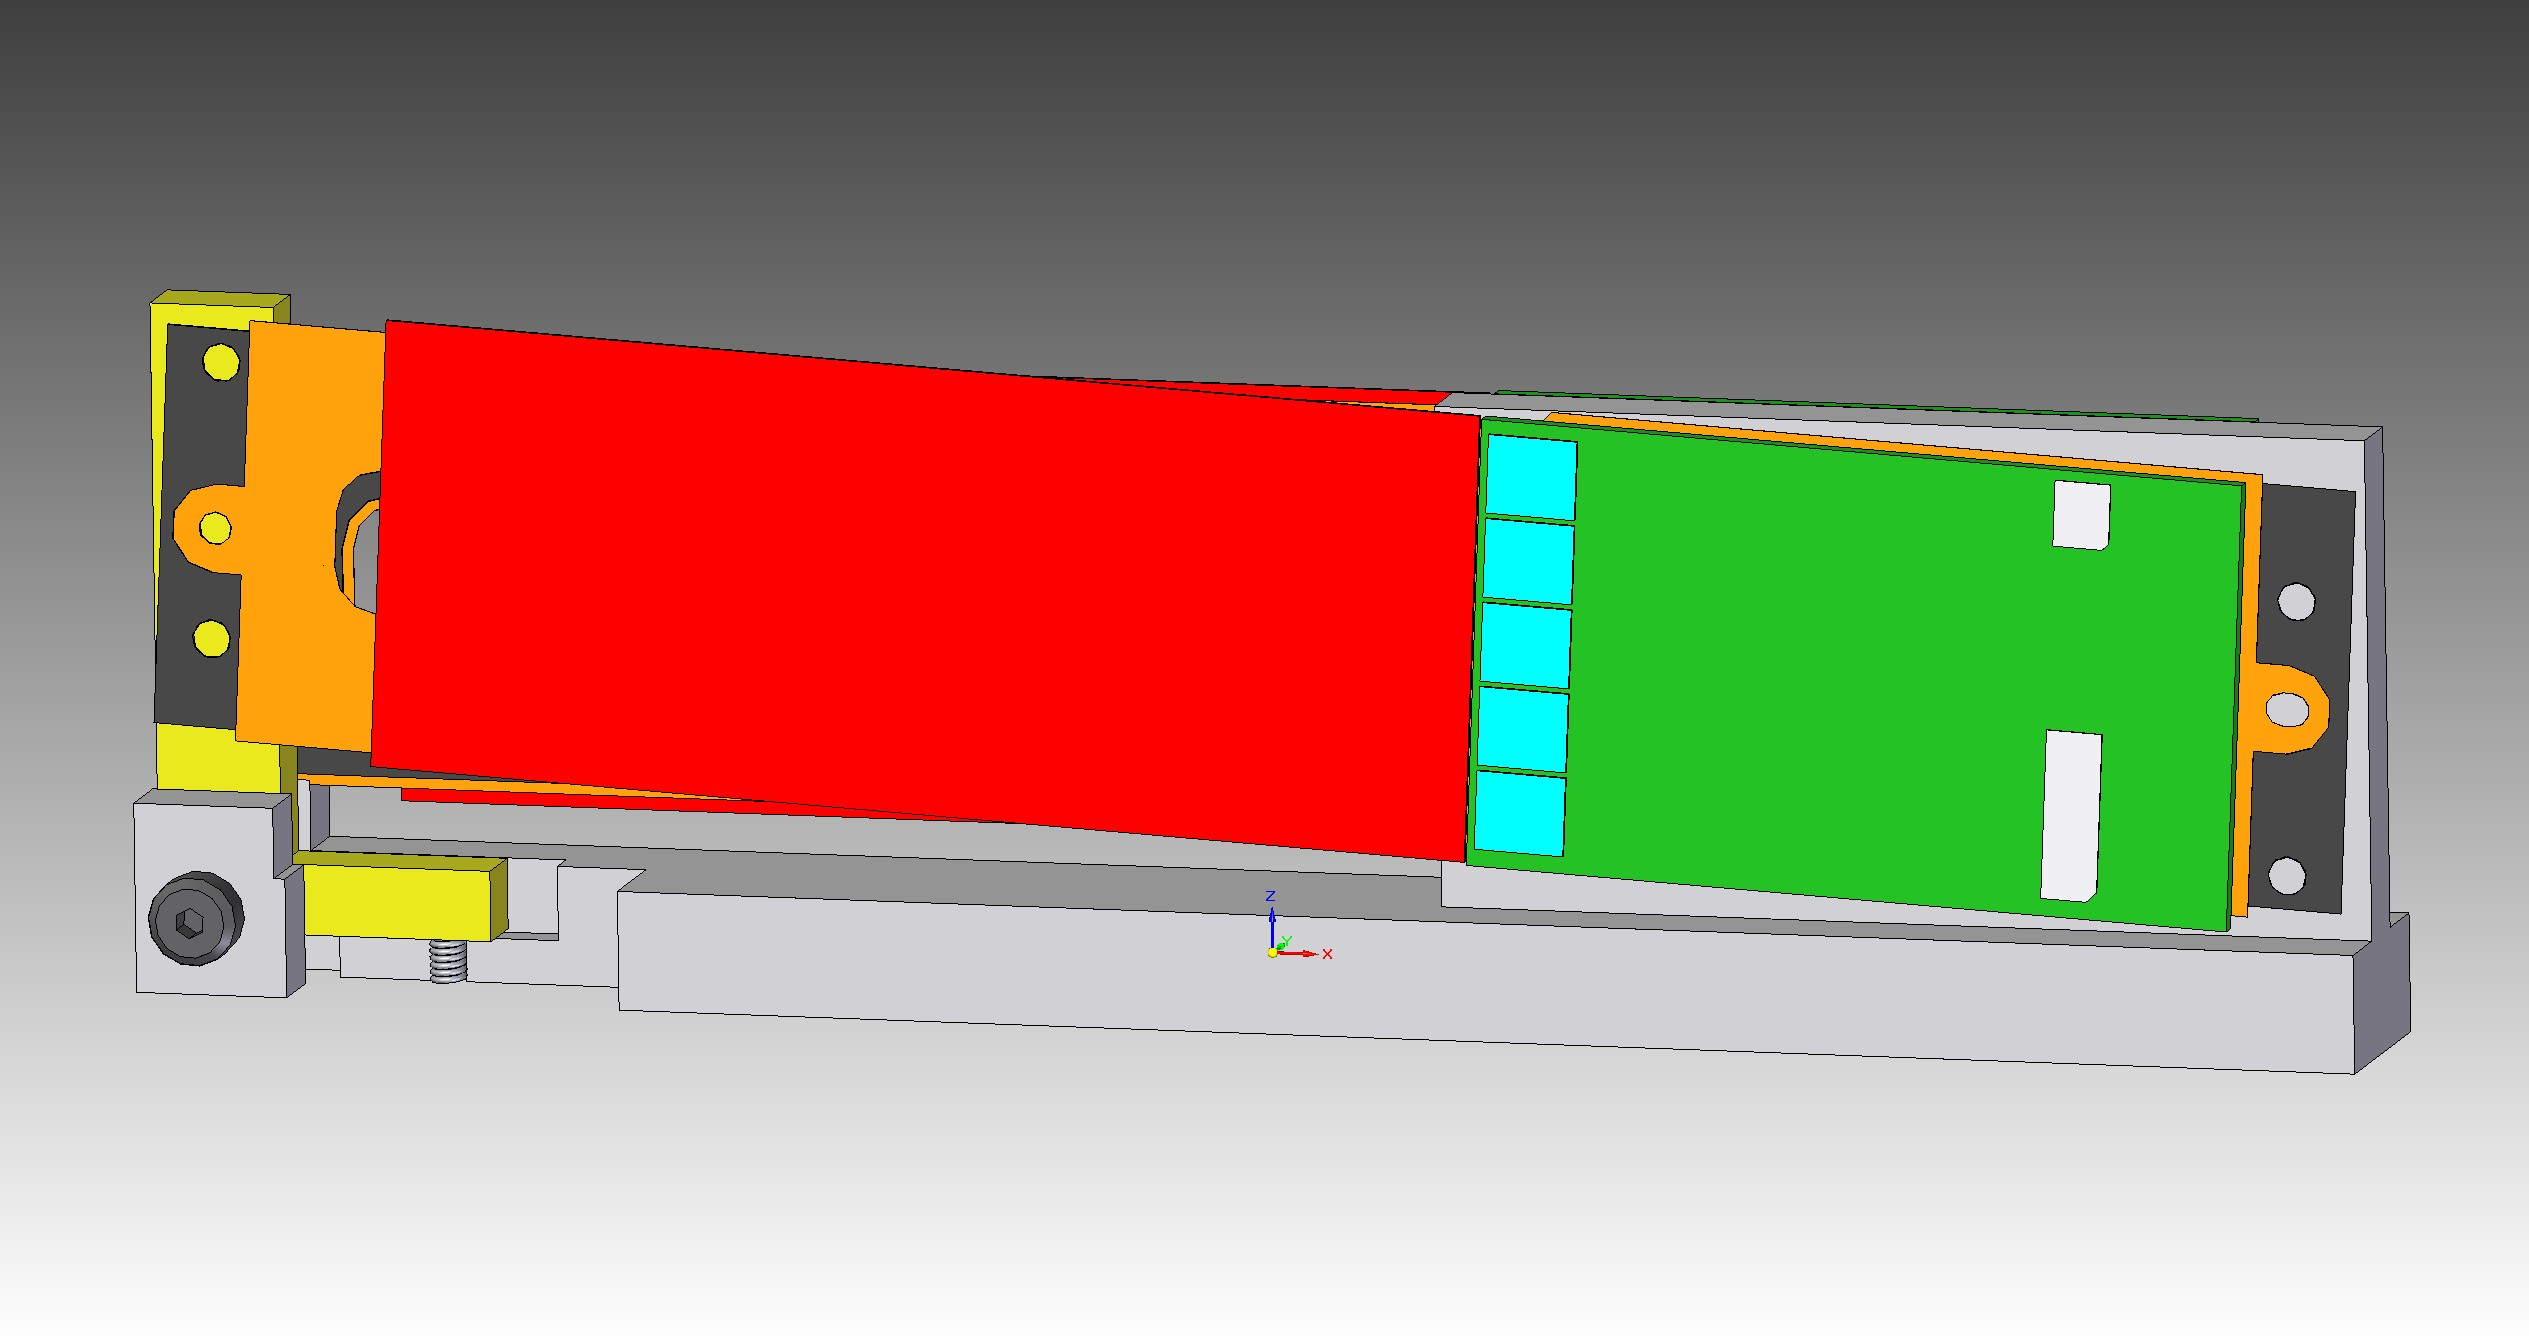
\includegraphics[width=0.5\textwidth]{detector/figs/svt_l123_drawing}
    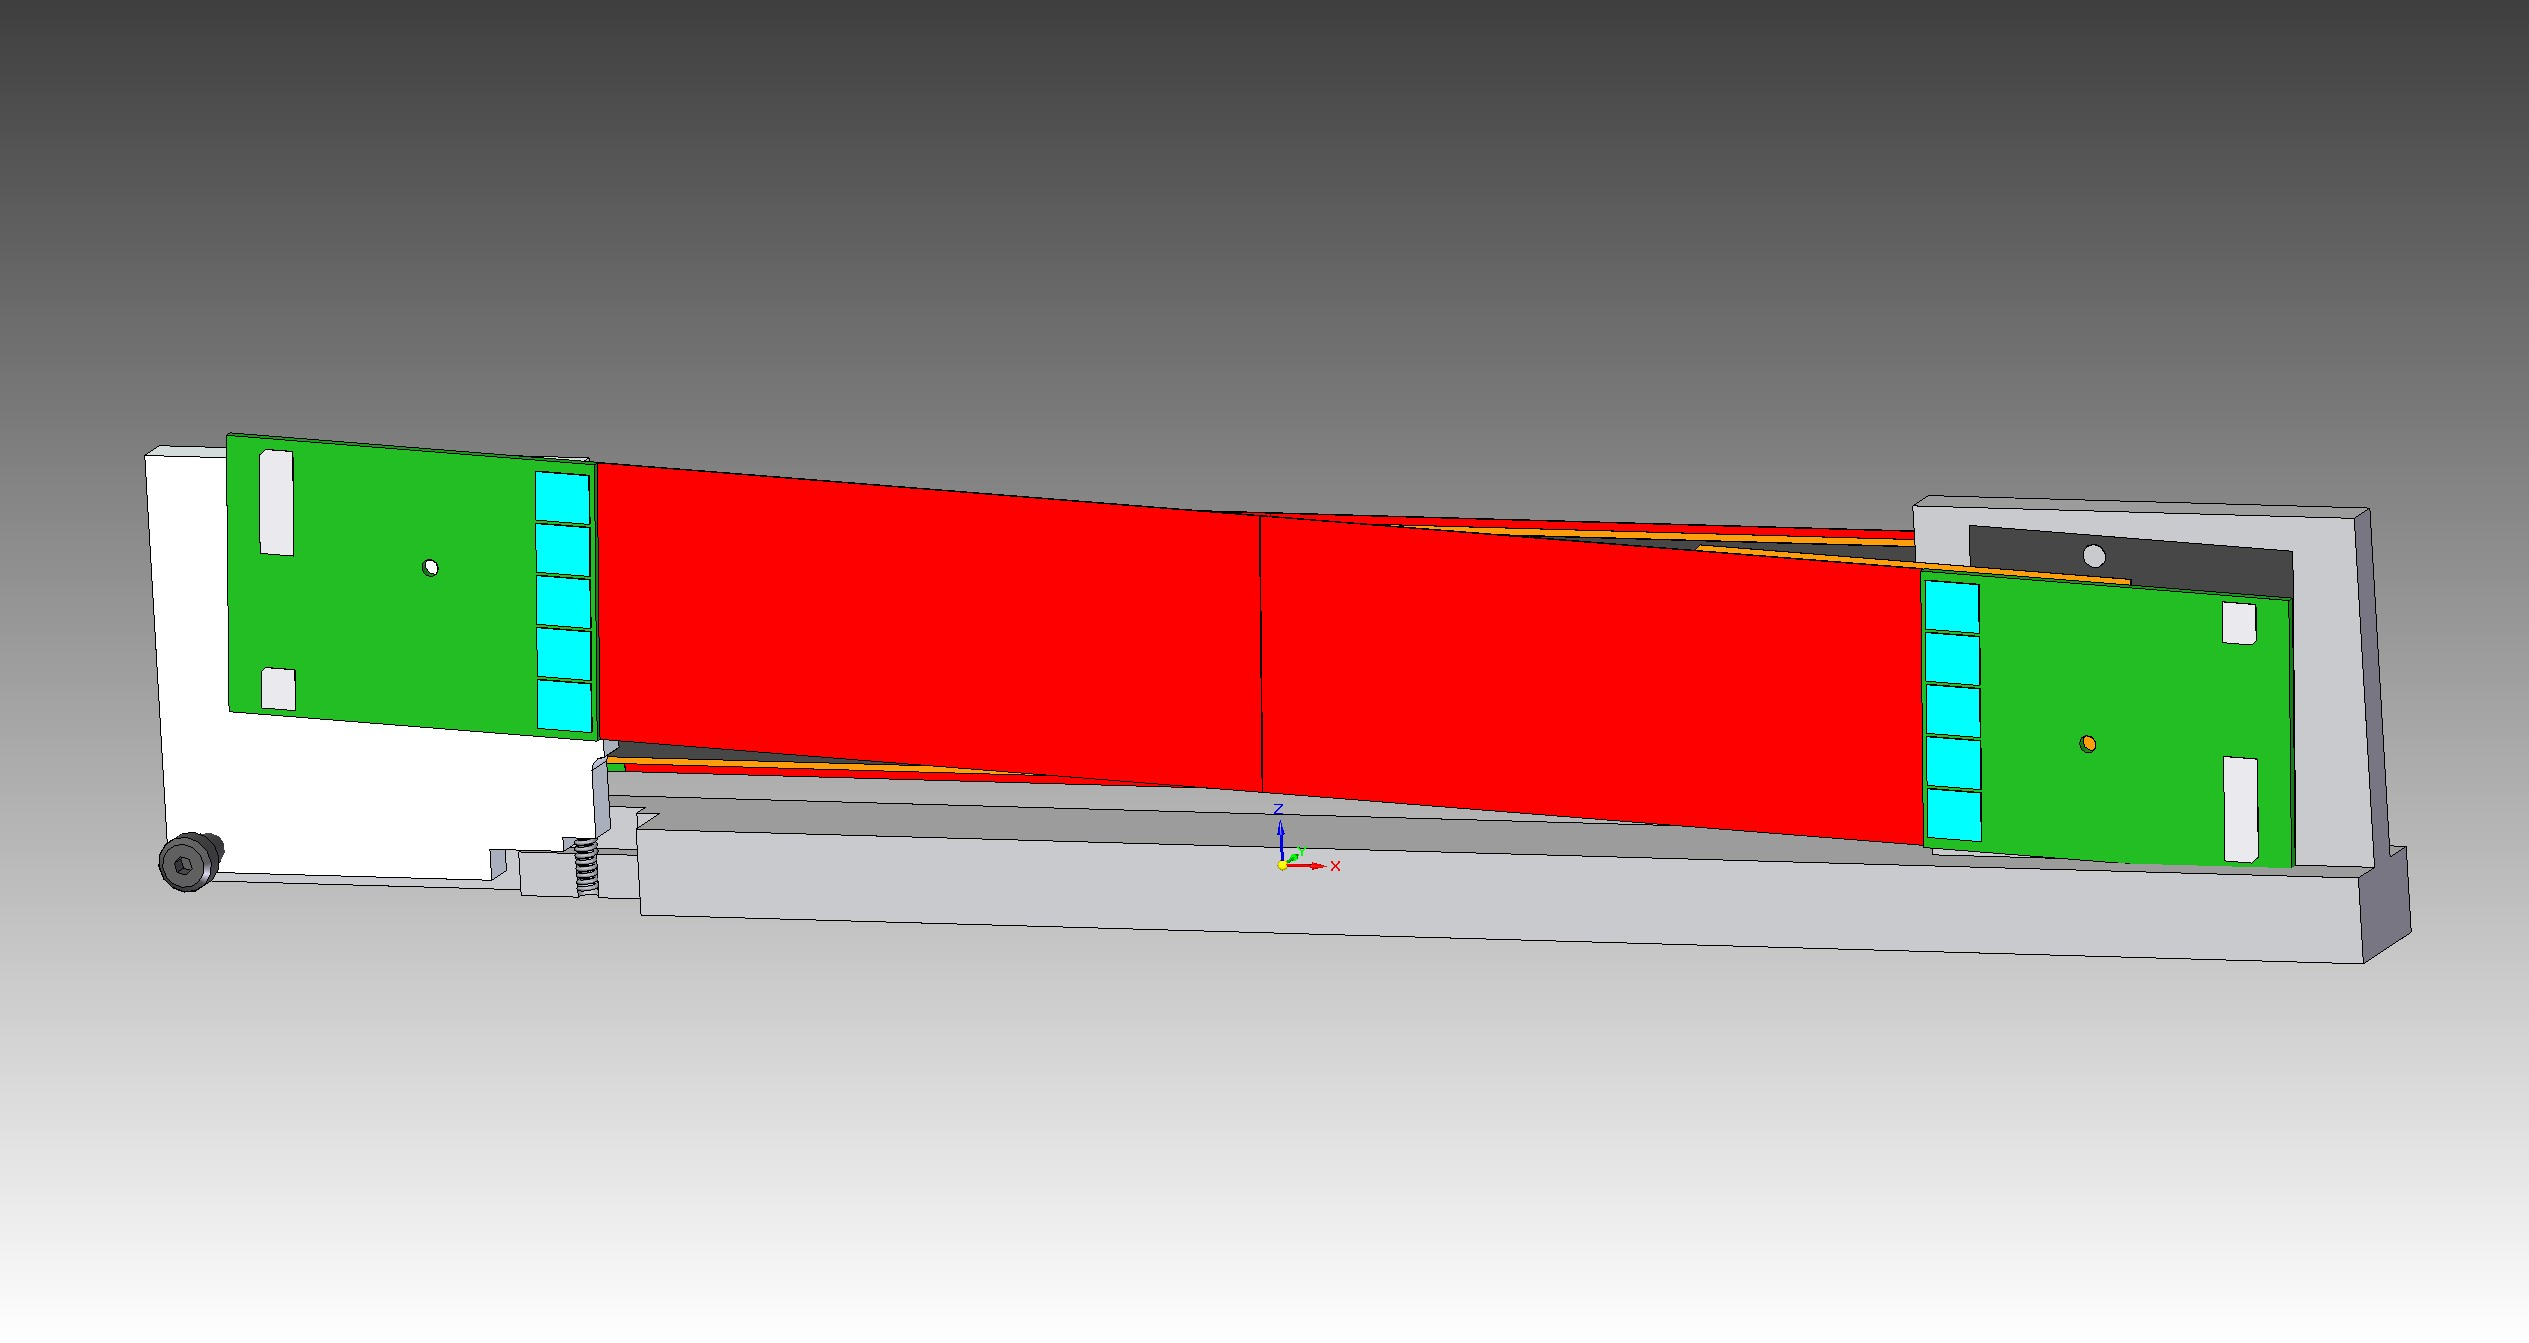
\includegraphics[width=0.5\textwidth]{detector/figs/svt_l456_drawing}
    \caption{Renderings of the L1--3 (left) and L4--6 (right) module designs, with cutaways to show the spring pivots that hold the silicon under constant tension.}
    \label{fig:svt-module-drawing}
\end{figure}

Three modules are mounted on a common aluminum support structure to form a ``U-channel.''
The sidewalls add to the rigidity of the U-channel and shield the sensors from thermal radiation.
The module mounting surfaces are recessed by the correct amounts to put the layers at the correct distances from the beam.
The SVT is divided into four U-channels: top and bottom L1--3, top and bottom L4--6.

\begin{figure}[htp]
    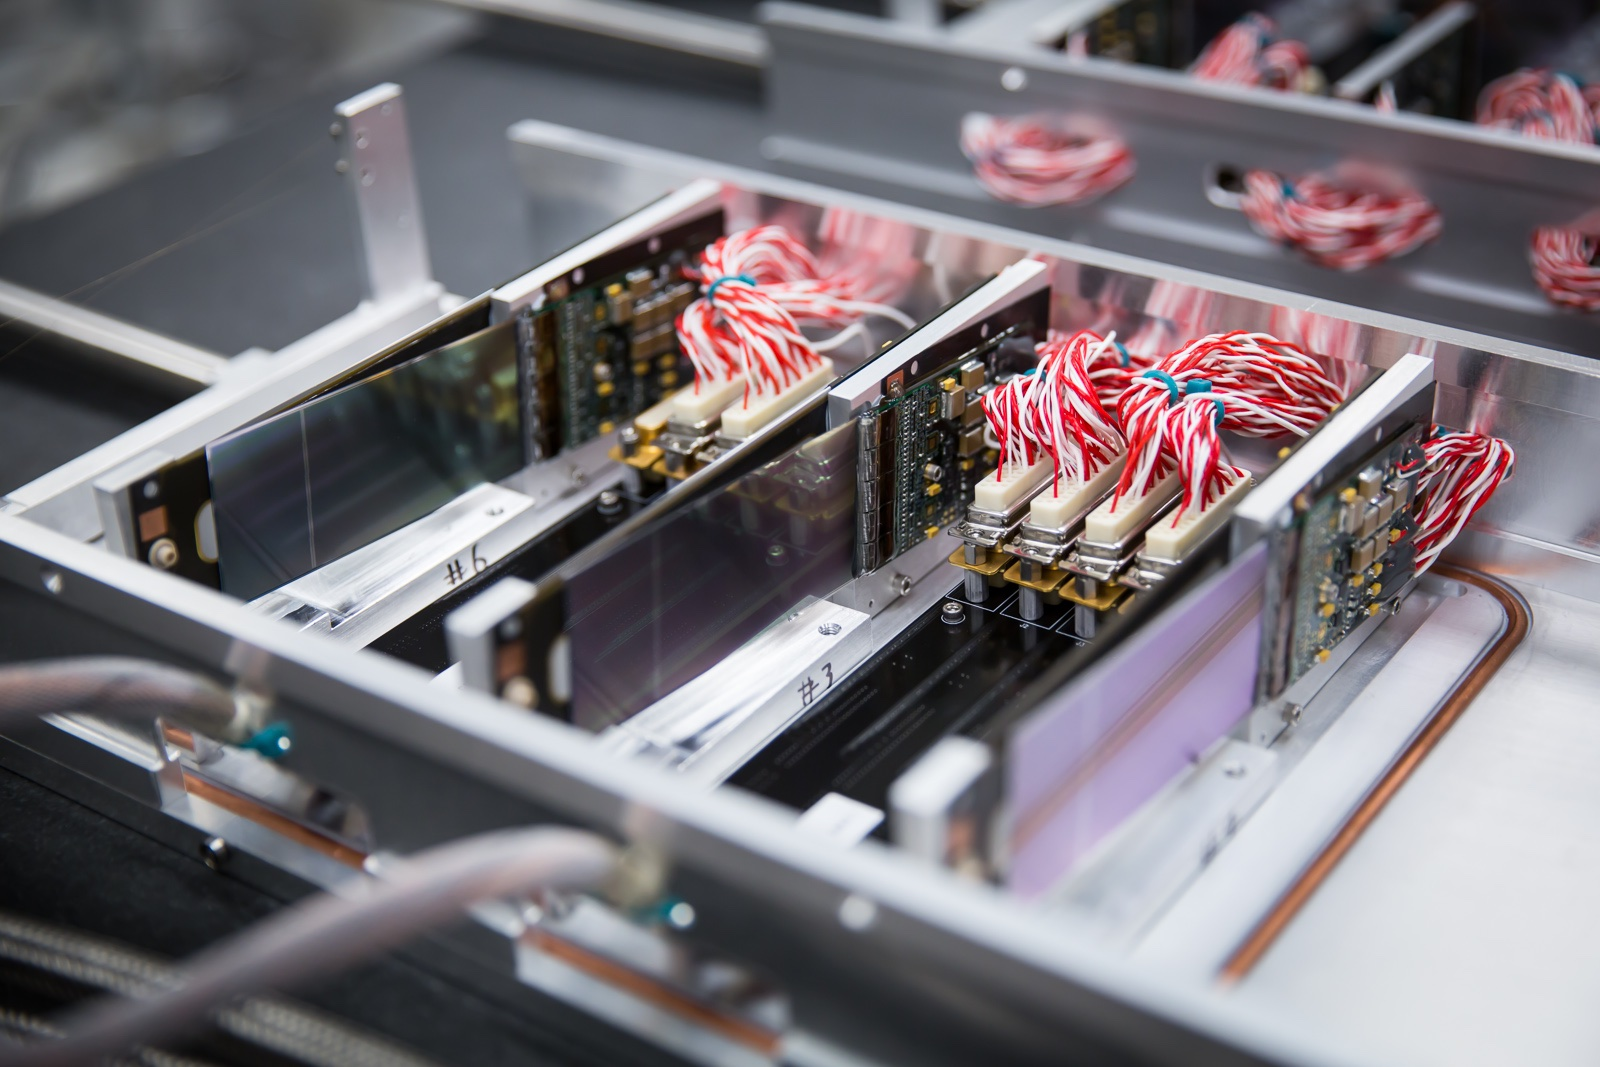
\includegraphics[width=\textwidth]{detector/figs/l123}
    \caption{One of two U-channels for L1--3, fully assembled.
    The beam direction is left to right; the scan wires and motion lever are visible on the left.}
    \label{fig:l123}
\end{figure}

\begin{figure}[htp]
    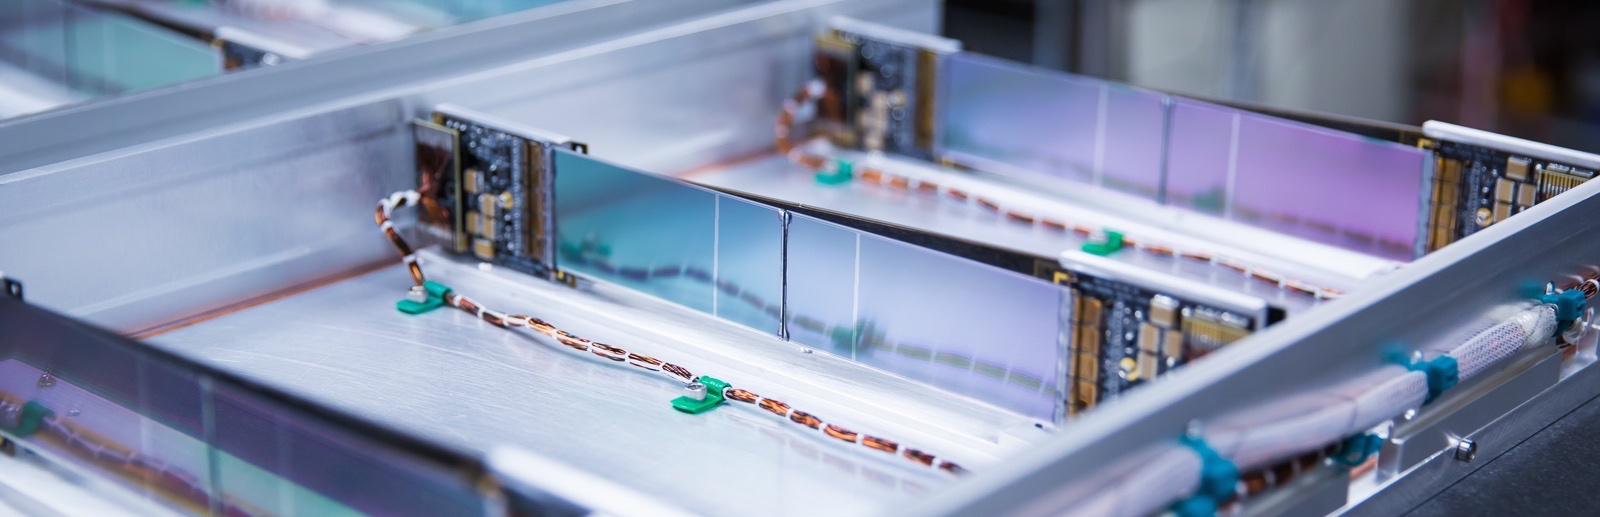
\includegraphics[width=\textwidth]{detector/figs/l456}
    \caption{One of two U-channels for L4--6, fully assembled.
    The beam direction is left to right.}
    \label{fig:l456}
\end{figure}

Each U-channel is supported at three points using kinematic mounts, which guarantee repeatable positioning when the U-channels are installed.
The L4--6 U-channels rest on three kinematic mounts.
The L1--3 U-channels rest on two kinematic mounts, which serve as a hinge at the downstream end of the U-channels, and are supported on the upstream end by motion levers which tilt the U-channels up and down.
In addition to modules, the L1--3 U-channels carry scan wires so that the beam position can be measured relative to the silicon.

\begin{figure}[htp]
    \begin{center}
    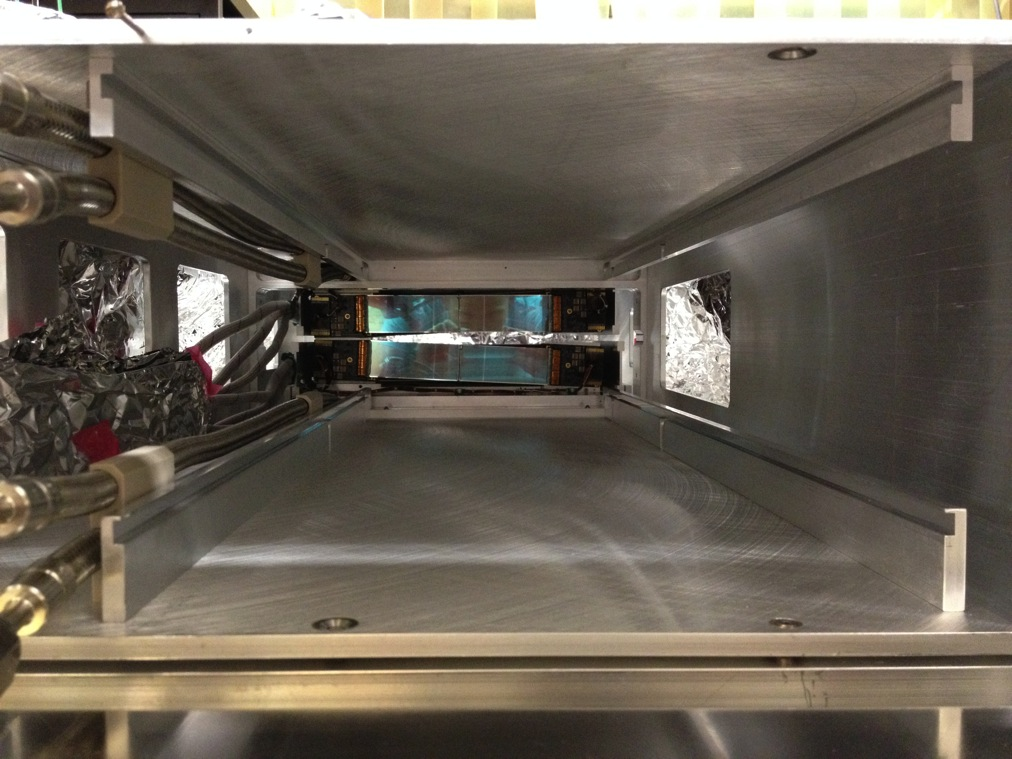
\includegraphics[width=0.8\textwidth]{detector/figs/drawers}
    \end{center}
    \caption{Inside the SVT box, looking downstream.
    The L4--6 U-channels are installed.
The rails for the L1--3 U-channels can be seen at the top and bottom. When the U-channels are installed, bearings on the U-channels roll along the horizontal slots until they drop down into the vertical slots, guiding the U-channel onto its kinematic mounts.
The cooling lines (in braided jackets) and cables (ends wrapped in foil) for the L4--6 U-channels are visible to the left.}
    \label{fig:drawers}
\end{figure}

\subsubsection{Survey}
\label{sec:svt_survey}

The SVT is surveyed to determine the positions of the sensors in the detector volume.
This serves two purposes.
First, surveying the SVT checks that it was assembled as designed, and allows adjustable components to be brought to their design positions.
Second, the precision of tracks reconstructed with the SVT is limited by the precision with which the sensor positions are known; the survey provides the initial knowledge of the detector geometry, which must be good enough to allow efficient track reconstruction, and close enough to the true geometry for track-based alignment (see Section \ref{sec:internal_alignment}) to work.

The basic tool for the SVT survey is a coordinate-measuring machine (CMM).
A CMM uses optical and/or touch probe measurements to locate target points in three dimensions.
%The silicon sensors were fabricated with fiducial markings that are easily measured optically.
%The bases of the pairing fixtures are a convenient reference frame for 
%The U-channels have conical fiducials meant for the module mounting surfaces and pins are simple shapes that can be located precisely with a touch probe, and the U-channels 

Because the SVT is assembled in a modular way, with repeatable positioning at each stage, the survey can be done in stages as well.
Each module is surveyed to find the positions of the silicon relative to the module mounting points.
Each U-channel is surveyed to find the positions of the module mounting points relative to the U-channel.
After the U-channels are installed in the SVT box, the SVT box is surveyed to find the positions of the U-channels relative to the SVT box; the U-channel kinematic mounts are adjusted during the survey to bring the U-channels to their nominal positions.
Finally, after the SVT box is installed in the pair spectrometer vacuum chamber, the SVT box is surveyed to find the position of the SVT box relative to the rest of the detector.

\subsection{Power and Data Acquisition}
\label{sec:power_daq}
The power and data paths for the SVT are constrained.
All signals must pass through a pair of 8-inch vacuum flanges at the upstream side of the analyzing magnet, so the number of signals has to be reduced.
The closest available rack for the SVT power supplies and DAQ is 20 meters from the alcove where HPS is installed, so the analog APV25 output signals have to be converted to digital optical signals.
Therefore HPS digitizes the signals and regulates the low-voltage power supplies inside the vacuum chamber, on frontend boards (FEBs) that are mounted on a cooling plate next to layers 1--3.

\begin{figure}[htp]
    %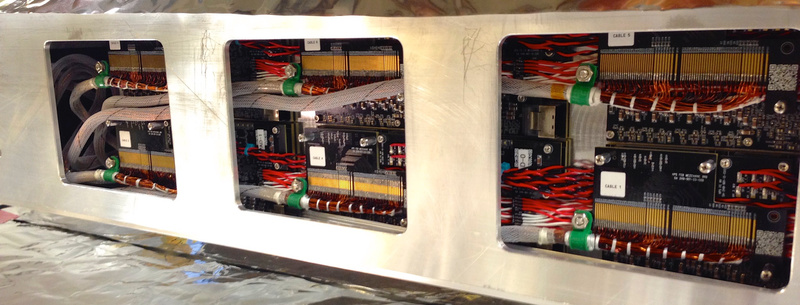
\includegraphics[width=\textwidth]{detector/figs/svt_febs}
    \begin{center}
    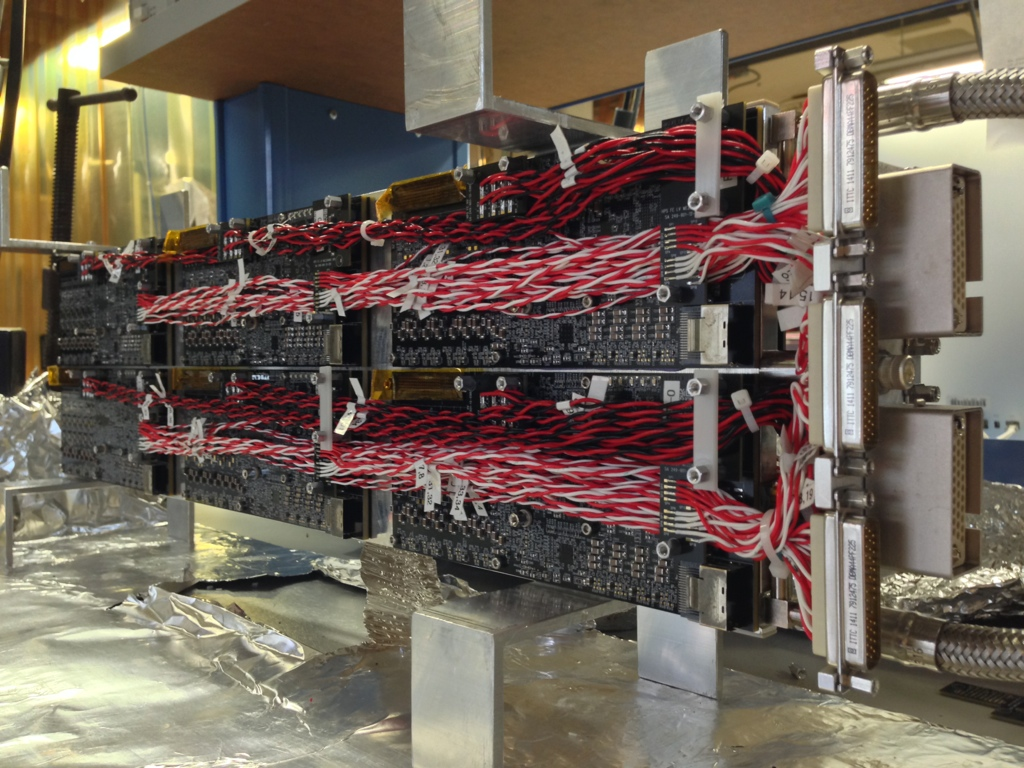
\includegraphics[width=0.8\textwidth]{detector/figs/febplate}
    \end{center}
    \caption{The SVT FEBs (frontend boards), mounted on their cooling plate. The red-and-white cables distribute low-voltage power to the FEBs; the red-and-black cables distribute high-voltage bias to the FEBs. The connectors for hybrid power, bias and data are covered with yellow Kapton tape. The mini-SAS connectors for high-speed data cables are at the bottom right of each FEB.}
    \label{fig:febplate}
\end{figure}

Each FEB can service four hybrids: a pair of L1--3 modules or a single L4--6 module.
A single bundle of impedance-controlled twisted pair magnet wire connects each FEB to its set of hybrids, carrying low-voltage power, high-voltage sensor bias, analog APV25 output signals, and digital control and trigger signals.

Each FEB digitizes the output signals from 20 APV25 chips.
Each differential current signal is converted to a voltage by a preamp and digitized by a 14-bit ADC.
Each FEB carries a single Xilinx Artix-7 FPGA, which packs the ADC data to be streamed off the FEB.
The FPGA also monitors the hybrid state and configuration.
All data and control signals are on a single high-speed data link, carried by a standard mini-SAS cable.

The FEBs also distribute low-voltage power to the hybrids.
A single voltage supplied to the FEB is split into four independent voltages (one per hybrid) using a combination of switching and linear voltage regulators.
This improves noise performance and reduces the number of voltages that must be passed into the vacuum chamber.
High-voltage sensor bias is also routed through the FEBs, but is passed through directly.

Two sets of cables connect the FEBs to the vacuum chamber flanges: mini-SAS cables carrying digital signals, and twisted pair cables carrying low-voltage power and high-voltage bias.
In both cases, the number of connections is too high for conventional vacuum feedthroughs.
Instead, HPS uses ``flange boards.''
Each board has a vacuum side and an air side, to which connections are made using solder or standard connectors.
The middle section of the board carries signal traces but is kept smooth; the board is then passed through a machined gap in the vacuum flange, and epoxy is poured to fill the space around the board: see Figure \ref{fig:flangeboard_test}.
The flange on beam-right carries two flange boards: one for low voltage and one for high voltage.
The flange on beam-left carries four signal flange boards (one of which is shown in Figure \ref{fig:flangeboard}), which use fiber transceivers on the air side to convert the electrical signals to optical signals.

\begin{figure}[htp]
    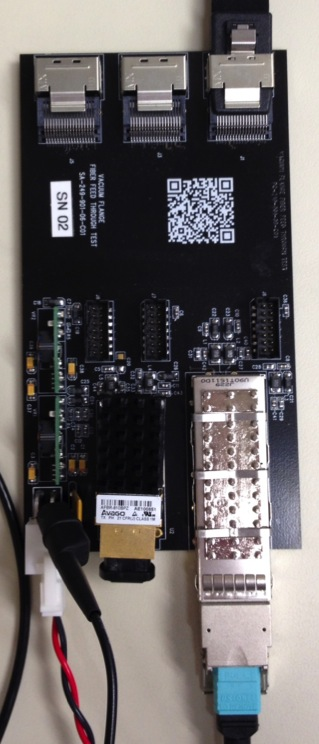
\includegraphics[angle=90,width=\textwidth]{detector/figs/flangeboard}
    \caption{One HPS signal flange board.
    The left side of the board operates in vacuum, and has three mini-SAS electrical connectors for high-speed data cables, which connect to the FEBs.
The right side of the board operates in air, and has two MPO multi-fiber connectors for data and control signals.}
    \label{fig:flangeboard}
\end{figure}

\begin{figure}[htp]
    \begin{center}
    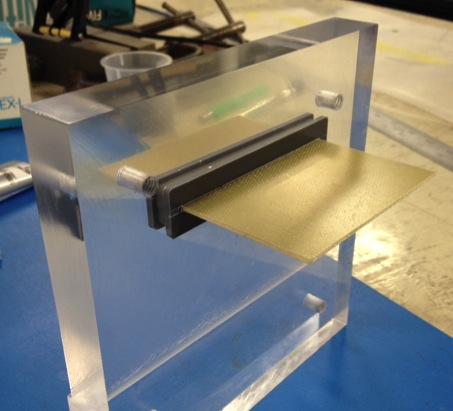
\includegraphics[width=0.7\textwidth]{detector/figs/flangeboard_test}
    \end{center}
    \caption{Test of the flange board potting process.}
    \label{fig:flangeboard_test}
\end{figure}

The low and high voltages for the SVT are supplied by Wiener MPOD power supplies.
The low-voltage supplies use sense lines to regulate the voltage actually supplied to the FEBs, and compensate for voltage drop in the cables.

The core of the SVT DAQ is the RCE platform.
This is a general-purpose DAQ system developed at SLAC.
The system is built on the ATCA (Advanced Telecommunications Computing Architecture) industry standard and is housed in a standard ATCA crate.

The data processing, trigger handling, and event building is done on a COB (Cluster On Board) blade, which carries a set of daughterboards: four DPMs (Data Processing Modules) and one DTM (Data Transport Module).
All of these are generic hardware that can be used for any experiment using the RCE platform.
The only HPS-specific hardware is the (RTM) Rear Transition Module, which interfaces the COB to the fiber bundles connected to the signal flange boards.
The SVT DAQ uses two fully loaded COBs and two RTMs.
Each DPM contains two data processing nodes, each of which runs a Xilinx Zynq system-on-a-chip which integrates an ARM processor (running the Linux operating system) and an FPGA.
The nodes can therefore process and reduce data on the FPGA at high speed, and perform high-level functions on the processor.
The DTM contains a single node, which handles timing and trigger distribution.
An implementation of the JLab TI (Trigger Interface) module is integrated in the DTM firmware for HPS.

\begin{figure}[htp]
    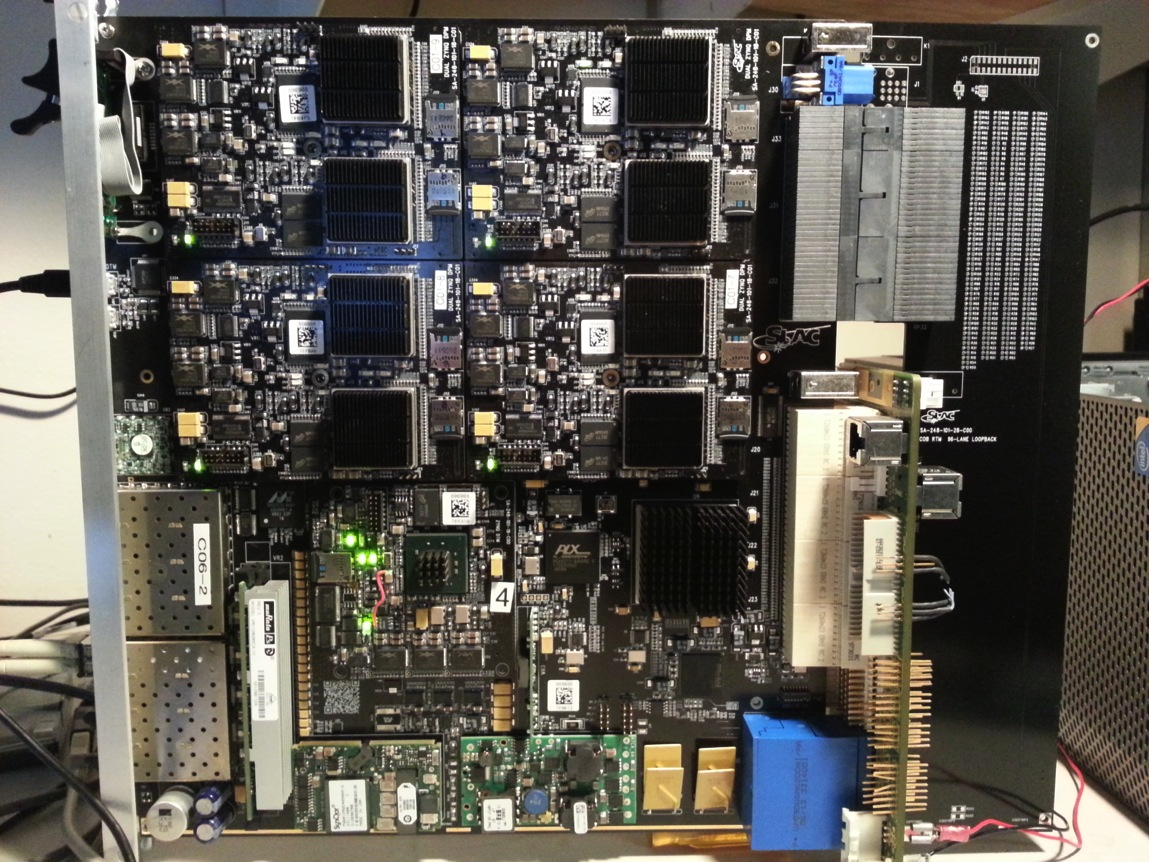
\includegraphics[width=\textwidth]{detector/figs/rce}
    \caption{The RCE system. The COB (Cluster On Board) blade on the left hosts four RCE (Reconfigurable Cluster Element) daughterboards, which perform the data processing. The RTM (Rear Transition Module) on the right interfaces with fibers carrying data from the flange boards. The COB and RTM would normally be housed in an ATCA crate.}
    \label{fig:rce}
\end{figure}

\subsection{Services}
\label{sec:svt_services}
All the services needed to operate the SVT --- motion, cooling, and power --- must be supplied from outside the vacuum.
These enter the vacuum through flanges on the upstream vacuum chamber.

Three linear shifts provide independent control of the upper and lower U-channels for layers 1--3, and the target frame.
Each linear shift is driven by a stepper motor; the three stepper motors are powered and controlled by a Newport XPS controller.
The motor turns a lead screw to create precise linear motion, which is transmitted inside the vacuum chamber through a bellows.

The SVT uses two independent cooling loops.
The silicon sensors need to be kept cold (below $0^\circ$ C) to prevent reverse annealing.
Reverse annealing is an effect where the performance of radiation-damaged silicon worsens after exposure to high temperatures.
The FEBs only need cooling to remove the heat they generate, and their cooling loop can run near room temperature.
%The SVT proper (sensors and hybrids, cooled through the U-channels) is kept near $-10^\circ$ C to prevent reverse annealing of the silicon.
%The FEBs (cooled through their cooling plate) are kept 

The SVT is cooled by circulating cooling fluid through copper lines that are pressed into the U-channels.
As discussed in Section \ref{sec:svt_mechanical}, the modules and half-modules are engineered to provide short and parallel cooling paths from the sensors and readout chips to the U-channels.
A low-viscosity fluid is required to keep flow rates high at low temperature; HPS uses Novec 7000, a hydrofluoroether compound.
The SVT chiller operates at a setpoint of $-20^\circ$ C.
The cooling flow is split between the top and bottom halves of the SVT before it enters the vacuum chamber through ceramic feedthroughs; the L1--3 and L4--6 U-channels are connected in series.

The FEBs are cooled by circulating distilled water through copper lines pressed into the FEB cooling plate.
The FEB components are kept in direct thermal contact with the cooling plate: the heat-generating components are on the side of the board that faces the cooling plate, and the plate has machined pockets lined with thermally conducting pads.
The FEB chiller operates at a setpoint of $25^\circ$ C.

Power provision to the SVT and FEBs is explained in Section \ref{sec:power_daq}.

\section{Electromagnetic Calorimeter and Trigger}
The HPS ECal is a homogeneous crystal calorimeter, containing 442 lead tungstate (PbWO$_4$) scintillating crystals.
The ECal is based on the CLAS Inner Calorimeter (IC); the crystals are reused from the CLAS IC, and the basic design of each crystal module is unchanged.
The mechanical and electronic design of the HPS ECal was led by the same IPN Orsay group that built the CLAS IC.

The crystals have a trapezoidal shape, 16 cm long, with front faces $1.3\times 1.3$ cm$^2$ and back faces $1.6\times 1.6$ cm$^2$.
Lead tungstate has a fast time response, which allows for good time resolution and high pileup tolerance.
An avalanche photodiode (APD) is glued to the back face of each crystal for readout.
Two LEDs (one red, one blue) are mounted on the front face of each crystal, and are used to monitor the stability of the readout gain and radiation damage to the crystals.

The ECal is split into top and bottom halves; each half contains 5 rows of 46 crystals, except for the innermost row which has 9 crystals removed to avoid the region of highest beam background (this gap in row 1 is known as the ``electron gap'').
The crystals are spaced as closely as possible.
Since the crystals are tapered, they fan out to the sides and an incident particle will typically not hit a crystal head-on.
Scintillator response is sensitive to the crystal temperature, so the ECal is surrounded by a thermal enclosure.
The innermost rows of crystals are 2 cm from the beam plane, and the front plane of the ECal is 139.3 cm from the nominal target position.

\begin{figure}[htp]
    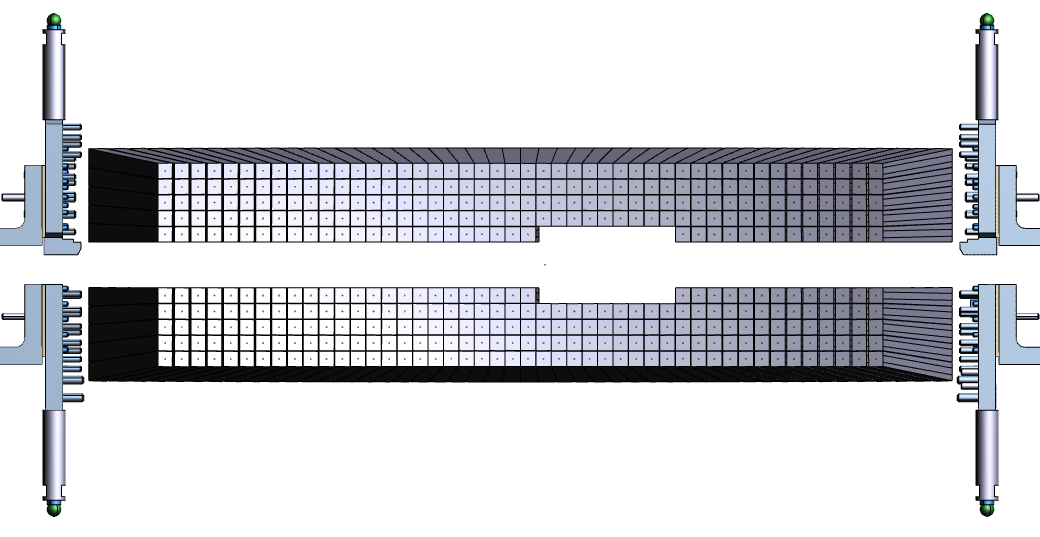
\includegraphics[width=\textwidth]{detector/figs/ECal}
    \caption{Beam's-eye-view of the ECal.
    18 crystals (the ``electron gap'') in the innermost rows are missing, to make space for the oval bulge in the ECal vacuum chamber (Figure \ref{fig:ecal_chamber}).
    The thermal enclosure that surrounds the ECal is not shown.}
    \label{fig:ecal}
\end{figure}

\begin{figure}[htp]
    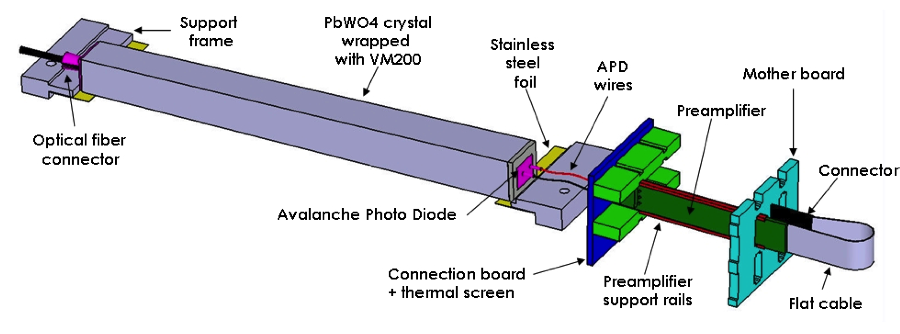
\includegraphics[width=\textwidth]{detector/figs/ecal_module}
    \caption{One ECal crystal with its readout electronics. The optical fiber was used in the CLAS IC for calibration and monitoring, but was removed for HPS. HPS uses LEDs mounted directly in front of the crystals.}
    \label{fig:ecal_module}
\end{figure}

\subsection{Readout and Trigger}
Each ECal crystal has its own preamplifier.
The preamp output signals are routed through a motherboard and out to cables, which connect to FADC250 digitizer boards in VXS crates.

The FADC250 (FADC for short) is a general-purpose readout board developed at Jefferson Lab.
Each FADC board has 16 input channels, which are digitized continuously to 12-bit precision at 250 MHz.
The digitized samples are stored in pipelines so they can be read out in response to a trigger.
Several readout modes exist, and the FADC has the capability to perform pulse integration or emulate a constant-fraction TDC, but HPS uses the readout mode that outputs a window of 100 samples around the trigger time.
This allows pulse fitting, for the best possible time resolution.

The FADC is also the first step in the trigger chain; the trigger chain is implemented entirely using VXS boards developed by Jefferson Lab as a general-purpose trigger framework for experiments at the lab.
The digitized samples are passed to an algorithm that continuously looks for threshold crossings, and integrates the signal amplitude within a fixed window around each threshold crossing.
The integrated amplitude is then converted to an energy using calibrated values of pedestal and gain.
Hits found in this way (crystal position, energy, time of threshold crossing) are reported to the Global Trigger Processor (GTP) every 32 ns.

The two GTP boards (one per ECal half) cluster the hits according to a simplified algorithm.
According to this algorithm, a cluster is a set of hits in a $3\times 3$ block of crystals, where the center hit is at least 50 MeV and is a local maximum in energy, and the other hits in the cluster are within 16 ns of the center hit.
Both GTP boards report clusters (center crystal, center hit time, number of hits, total energy) to the single Subsystem Processor (SSP) board.

The Subsystem Processor (SSP) makes the trigger decision.
For the HPS physics trigger, the clusters from the two halves of the ECal are paired up, and each pair is tested against the defined trigger cuts.
If a pair meets the trigger requirements, a trigger is sent to the Trigger Supervisor board (TS), which then distributes the trigger to the Trigger Interface (TI) boards installed in all detector readout subsystems.
If any subsystem is not ready to accept a trigger, or if the trigger follows too closely after another trigger (as defined by rules configured in the TS), the TS will reject the trigger.
The fraction of time for which the TS rejects triggers (deadtime) is monitored and recorded.

A total of six trigger types are defined in the SSP.
The HPS physics trigger is nicknamed ``pairs-1'' and is detailed in the next section.
A looser variant of the same trigger is nicknamed ``pairs-0'' and is used for diagnostics.
A single-cluster trigger tuned to trigger on electrons near the beam energy (elastic scatters) is called ``singles-1,'' and a looser variant is ``singles-0.''
To keep the rates of ``pairs-0,'' ``singles-1'' and ``singles-0'' triggers low as a fraction of the total trigger rate, they are prescaled so only one in $2^N$ ($N$ in the range of 7 to 13, depending on the trigger) of each trigger is accepted.
A pulser trigger generates a constant rate of triggers at 100 Hz regardless of detector conditions.
A ``calibration'' trigger is used for cosmic ray calibration of the ECal when the beam is off, triggering on a pair of scintillator paddles mounted under the ECal.

The total trigger rate during normal operations in the 2015 run was roughly 19 kHz, of which 16.6 kHz was pairs-1.

\subsection{Trigger Cuts}
\label{sec:trigger_cuts}

The HPS physics trigger is tuned to maximize efficiency for heavy photon decays: $e^+e^-$ coincidences with total energy near the beam energy.
For reasons explained below, there is no attempt to impose a minimum total energy requirement.
The main single-particle backgrounds are elastic scatters (electrons with energy near the beam energy) and bremsstrahlung photons.
The main two-particle background is wide-angle bremsstrahlung, where both the electron and photon hit the ECal.

A cluster reported to the SSP will not have energy equal to the incident particle, or even to the energy the full HPS reconstruction would compute for that cluster.
First, the FADCs are calibrated such that the reported energy of a hit equals the energy deposited in the crystal; whenever a particle showers in the ECal, some energy is absorbed in the vacuum flange in front of the ECal, penetrates through the back of the ECal, or escapes through the gaps between crystals.
These effects are compensated for in the full reconstruction but are ignored in the trigger.
Second, the GTP imposes a $3\times 3$ limit on the dimensions of a cluster, even though a single shower can deposit energy in a larger area.
For these reasons, the energy thresholds used in the trigger cuts are rather lower than would be expected based on true particle energies.

Furthermore, many particles hit the ECal in or near the innermost row of crystals.
For these particles, much of the shower is lost in the beam gap and the energy of the cluster can be much less than the particle energy.
Since these may still be desirable events (many decays from lower-mass heavy photons land in the innermost row of crystals), the trigger cuts mostly avoid imposing strong minimum requirements on cluster energy or total energy.

The time coincidence between the top and bottom clusters is required to be within 12 ns.
This allows for time walk; since the hit time reported by the FADC is a simple threshold crossing with a low threshold, time walk can be substantial.

The SSP applies an initial requirement on the energy and size of each cluster; it only considers clusters with energy between 54 and 630 MeV, and at least 1 hit.
For a pair, the sum of the cluster energies is required to be between 180 and 860 MeV, and the difference is required to be less than 540 MeV.
The minimum hit requirement is obviously trivial; the minimum cluster energy requirement is largely redundant with the GTP requirement on the center hit energy.
Of the other requirements, the most important is the maximum energy sum requirement: most of the events rejected by this cut are pairs of two beam-energy electrons.

The coplanarity cut is intended to select $e^+e^-$ events.
On average, $e^+e^-$ events should be symmetric around the beam axis (the line pointing along the beam direction at the target, starting at the beam spot).
Events with two electrons will usually have both clusters on beam-right, and will fail this cut.
The cut requires that the two clusters be on opposite sides of the beam axis: the azimuthal angle of each cluster is computed relative to the beam axis, and the difference between the two angles is required to be within $\pm 30^\circ$ of $180^\circ$.
(In practice, this cut is implemented as a mask of pairs of cluster positions that satisfy this cut.)

The energy-distance cut acts on the lower-energy cluster of the pair, and imposes the requirement $E_{low}+(5.5\text{ MeV/mm})r_{low}>600$ MeV, where $E_{low}$ is the cluster energy and $r_{low}$ is the cluster distance from the beam axis.
Restated as $E_{low}/(600\text{ MeV})+r_{low}/(600/5.5\text{ mm})>1$, the effect of this cut is to reject the pair if the lower-energy cluster is low-energy and close to the beam axis.
This primarily rejects wide-angle bremsstrahlung events, where the photon is typically the lower-energy particle, and is usually close to the beam axis.
The cut also rejects beam-energy electrons that hit close enough to the ECal edge that most of the energy is lost; these would pass the cluster energy cuts, but are closer to the beam axis than a genuine low-energy charged particle would be.

\begin{table}[htp]
    \begin{center}
        \caption{Trigger cuts for the ``pairs-1'' trigger.
        %$r$ and $\phi$ are defined relative to the photon line 
        }
        \begin{tabular}{lc}   
            \hline \hline
            Time difference & $|t_{top}-t_{bot}|\le12$ ns \\
            Cluster energy & $54<E<630$ MeV \\
            Cluster size & $N_{hits}\ge 1$ \\
            Energy sum & $180<E_{top}+E_{bot}<860$ MeV \\
            Energy difference & $|E_{top}-E_{bot}|<540$ MeV \\
            Coplanarity & $|\phi_{top}-\phi_{bot}-180^\circ|<30^\circ$ \\
            Energy-distance cut & $E_{low}+(5.5\text{ MeV/mm})r_{low}>600$ MeV \\
            \hline \hline
        \end{tabular}
        \label{tab:trigger_cuts} 
    \end{center}
\end{table}


\chapter{Event Reconstruction and Selection}
%This chapter covers the HPS event reconstruction with 

\section{Reconstruction}
\subsection{Tracking}
\label{sec:track_recon}

\subsubsection{Hit Reconstruction}
\label{sec:svt_hit_recon}

\subsubsection{Track Finding and Refit}
\label{sec:track_finding_refit}
track finding

GBL refit

\subsection{Vertexing}
\label{sec:vertex_recon}
Pairs of tracks are vertexed using a fast vertex fit that finds the best-fit vertex position and track parameters based on the track parameters and covariance matrices, and optional additional vertex constraints \cite{billoir_fast_1992}.

The HPS vertex reconstruction uses constraints on the $x$, $y$, and $z$ location of the vertex.
All constraints are limited by the vertex resolutions in those directions; the $x$ and $y$ constraints are limited by the beamspot size, and the $z$ constraint is limited by knowledge of the target position, but these are all smaller than the vertex resolutions.
%Three types of constraints are used, all using knowledge about the target and/or beamspot.
The ``$z$-constrained'' fit requires that the vertex be consistent with the $z$ location of the target.
The ``target-constrained'' fit requires that the vertex be consistent with the $z$ location of the target, and with the $x$ and $y$ location of the beam spot.
The ``beamspot-constrained'' fit requires that the vertex position and momentum are such that the vertex momentum points back to the beamspot at the target $z$.

\subsection{Clustering}
\label{sec:clustering}

\subsection{Track-Cluster Matching}
\label{sec:matching}
\section{Tracker Performance and Alignment}
\subsection{Internal Alignment}
\label{sec:internal_alignment}
millepede
\subsection{Elastic Electrons}
\label{sec:target_z}
\subsection{M{\o}ller Electrons}
\label{sec:mollers}

\section{\texorpdfstring{$e^+e^-$}{e+e-} Selection Cuts}
\label{sec:event_selection}
After reconstruction, all possible $e^+e^-$ pairs in the event are tested against a set of cuts.
There is no explicit requirement that the electron and positron be the pair of particles that caused the trigger.
There is also no fiducial requirement, since the inner edge of the detector acceptance is key for sensitivity to low-mass heavy photons.
The base selection is intended to remove accidental coincidences from the pair sample; the pair sample should contain only events where the electron and positron originate in the same interaction.

The ``pairs-1'' trigger is the HPS physics trigger, described in Section \ref{sec:trigger_cuts}.
It is tuned to accept $e^+e^-$ pairs, and is the overwhelming majority of the event rate (16.6 kHz out of 19 kHz).

The electron and positron are required to be in opposite halves of the detector: this cut is implemented as a requirement that the $y$-coordinates of the two clusters have opposite signs.
The trigger requires a top-bottom coincidence, so repeating the requirement as an event selection cut does not reduce the efficiency.
This cut eliminates any possibility of confusion in the track or cluster reconstruction, since the hits from the electron and positron are guaranteed to be well separated.
%A heavy photon can have enough transverse momentum that both decay products land in the same half of the detector, but the rate is low.

Track-cluster matching is important for two reasons: the cluster time resolution is better than the track time resolution, and track-cluster matching eliminates many misreconstructed tracks.
Two checks are done on the quality of the track-cluster matching for both particles.
First, a cut is made on the $\chi^2$ of the track-cluster match; this is a requirement on the distance between the cluster position and the track extrapolation to the ECal.
Second, a cut is made on the track-cluster time difference.
Since the track and cluster times are referenced differently (the track time is relative to the trigger time, and the cluster time is relative to the start of the ECal readout window), a constant offset of 43 ns is subtracted.

Three more simple cleanup cuts are applied.
A loose track quality cut is applied on the $\chi^2$ of each GBL fit; this is only meant to reject very poor track fits.
Elastically scattered electrons with $p(e^-)\approx E_{beam}$ are the main pileup background in the tracker, and are rejected with a maximum momentum requirement on electrons.
A momentum sum cut rejects pairs with a momentum sum too far in excess of $E_{beam}$; this further reduces the rate of random coincidences with elastic electrons.

The last cleanup cut is a cut on the cluster time difference.
This selects time coincidences.
The track time difference could be used similarly, but the cluster time resolution is better.

Finally, a ``radiative cut'' is applied for heavy photon analyses.
This is a minimum requirement on the momentum sum, at $0.8E_{beam}$.
As shown in Section \ref{sec:signal_kinematics}, most heavy photons and radiative tridents are produced with energy near $E_{beam}$; the radiative cut keeps most of these and rejects the Bethe-Heitler tridents that dominate at low momentum.

\begin{table}[ht]
    \begin{center}
        \begin{tabular}{lc}   
            \hline \hline
            Trigger type & ``pairs-1'' trigger \\
            Run and event quality & see Section \ref{sec:luminosity} \\
            Top-bottom requirement & $\sign(y_{cl}(e^-))\neq\sign(y_{cl}(e^-))$ \\
            Track-cluster matching (position) & $\chi^2_{match}<10$ \\
            Track-cluster matching (time) & $|t_{cl}-t_{trk}-43|<4$ ns \\
            Track quality & $\chi^2_{trk}<50$ \\
            Elastics cut & $p(e^-)<0.75E_{beam}$ \\
            Momentum sum cut & $p_{tot}(e^+e^-)<1.15E_{beam}$ \\
            Cluster time coincidence & $|t_{cl}(e^-)-t_{cl}(e^+)|<2$ ns \\
            Radiative cut & $p_{tot}(e^+e^-)>0.8E_{beam}$ \\
            \hline \hline
        \end{tabular}
        \caption{Base pair selection cuts for HPS.}
        \label{tab:basic_cuts} 
    \end{center}
\end{table}

\subsection{Tuning Cuts}
The cuts are tuned on the data, using the cluster time difference to separate ``good'' and ``bad'' events.
Pairs with large cluster time difference ($|t_{cl}(e^-)-t_{cl}(e^+)|>3$ ns) are accidental coincidences; pairs with small cluster time difference ($|t_{cl}(e^-)-t_{cl}(e^+)|<1$ ns) are dominated by true time coincidences.
An effective cut should reject pairs with large cluster time difference, and not pairs with small cluster time difference.

Figure \ref{fig:basecut_performance} shows the effect of the cuts on the distribution of cluster time differences.
This distribution is the sum of the distributions of true coincidences and random coincidences.
The distribution of true coincidences is a single peak with shape determined by the time resolution, and the distribution of random coincidences is the sum of multiple peaks spaced by the 2 ns beam period, with a slowly varying envelope shaped by the efficiencies of the trigger and track reconstruction.
If (as is the case for all cuts shown in the figure) a cut is not directly sensitive to the cluster time difference, and yet suppresses the outer peaks more than the central peak, it must be rejecting random coincidences.
%Each cut rejects more of the out-of-time events than the in-time events.
%Since the cluster time coincidence cut is the only cut that uses the cluster time difference, this implies that the fraction of accidental coincidences in the central peak decreases

The cluster time coincidence cut is applied after the other cuts, and selects only the central peak.
The rate of random coincidences contaminating the central peak can be estimated from the outer peaks: the fraction of random coincidences after the event selection cuts is roughly 1.5\%.

\begin{figure}[ht]
\begin{center}
    \includegraphics[width=0.6\textwidth,page=2,angle=-90]{recon/figs/basecutplots}
\end{center}
    \caption{Cumulative effect of the different pair selection cuts on pair-1 events passing the top-bottom requirement and radiative cuts.
    The ratio of out-of-time to in-time events (outer peaks to central peak) decreases as cuts are applied (going from the black to the magenta distributions).
    }
    \label{fig:basecut_performance}
\end{figure}

\section{Run Quality, Event Quality, and Data Normalization}
\label{sec:luminosity}
All the data used in the analysis should have the same detector conditions and efficiencies: this is ensured by appropriate selections of runs and events.
The HPS data is divided into runs, which are roughly two hours each unless interrupted by DAQ problems.
All ``golden runs'' included in this analysis have the same configuration for the HPS setup: the tungsten target with design thickness of 0.125\% $X_0$, nominal beam current of 50 nA, the trigger cuts listed in Section \ref{sec:trigger_cuts}, and the SVT position at nominal (layer 1 silicon at 0.5 mm from the beam).

A more fine-grained run quality selection is necessary because even a golden run can include substantial amounts of data that were recorded without the detector being in the desired configuration: a good-quality run can have periods of poor-quality data.
The most common situation is a beam trip.
According to the procedures that were followed by shift workers in the 2015 run, the high-voltage bias to the SVT sensors was lowered when the beam was lost, and bias was only restored after the beam returned.
Furthermore, if the trip was determined to be caused by the halo counter FSD (see Section \ref{sec:beam_quality}), the SVT would be moved out to 1.5 mm from the beam, and only moved back in after the beam returned.
The result is that the SVT would not be in its normal configuration after beam restoration: the bias would be low, and the SVT position might be away from nominal.
Between beam restoration and the restoration of SVT bias and position, data would be recorded but it would not be reconstructable, since at low bias the SVT would not see hits, and at a position away from nominal the SVT alignment would not be correct.

The SVT bias and position history are recorded in a database, and the database is used to find the time intervals when the SVT was in its nominal configuration.
These time ranges are then used to select events with good run quality.

There are additional effects in the SVT that can affect event quality, and can be identified on an event-by-event basis.
The SVT DAQ can enter an error state during a run, which affects all data for the rest of the run for a single sensor; the error state is flagged in each event, so these events are easy to reject.
Roughly 40\% of the data used in this analysis was recorded before the correct setting for the APV25 latency was found; with the incorrect setting, if an event occurs too late relative to the APV25 clock, the SVT hits will not pass the data reduction threshold.
This affects 1/3 of the events in these runs, and the events are identified and rejected based on their trigger timestamps.
Finally, a small fraction (3.5\%) of events in every run have elevated noise in the SVT because the APV25 pipelines were being filled as the APV25 was outputting the digital header for a previous event.
This effect is called ``burst-mode noise'' after the APV25 feature that allows a trigger to be received while a previous event is being read out.
Events with burst-mode noise are identified by counting the number of isolated (no neighboring strips with hits) low-amplitude hits: most normal events have no such hits, and the noisy events have many (tens to hundreds), so this analysis rejects events with 3 or more isolated low-amplitude hits.


Since the expected rate of heavy photons can be normalized to the data, a precise measurement of the integrated luminosity is not critical to the analysis.
Normalizing the data to the integrated luminosity is still essential for understanding the detector efficiencies and comparing the data to the cross sections of known processes.
In order for the integrated luminosity to be useful, it should be corrected for the run and event quality selections.

The luminosity is the product of the beam current, target thickness, and experiment livetime.
The beam current is measured by a Faraday cup, as described in Section \ref{sec:beamline_hallb}.
The target thickness is taken from measurements made during target assembly.
The experiment livetime is the product of the trigger livetime and the SVT DAQ efficiencies (latency and burst-mode noise) explained above.

Section \ref{sec:trigger} explains the two measurements of trigger livetime.
One, from the Faraday cup, measures the fraction of the integrated beam charge which was accumulated with the DAQ live.
The other, from the pulser trigger, measures the fraction of time for which the DAQ was live.
The Faraday cup is more precise, both because it accounts correctly for fluctuations in beam current, and because it has less statistical uncertainty (the Faraday cup scaler rate is roughly 45 kHz at 50 nA, much higher than the 100 Hz frequency of the pulser trigger).
However, the pulser livetime is recorded more frequently (every second, as compared to every 4-5 seconds), and this makes it easier to integrate the luminosity over the run quality time ranges.
A comparison of the Faraday cup and pulser livetimes shows agreement at the 1\% level or better, so the pulser livetime is acceptable.

The luminosity is integrated over the time ranges identified (as explained above) for good SVT bias, good SVT position, and SVT DAQ error status.
The resulting integrated luminosity is appropriate for comparisons with Monte Carlo samples: it assumes an always-on beam, a detector always in its nominal state, and a DAQ that always takes good data.

\subsection{Rate Comparison with Monte Carlo}
\label{sec:rates}

\begin{figure}[ht]
\begin{center}
    \includegraphics[width=0.6\textwidth,page=22,angle=-90]{recon/figs/wabratioplots}
\end{center}
    \caption{Momentum sum $p_{tot}(e^+e^-)$ for data (black), Monte Carlo samples of tridents (red) and wide-angle bremsstrahlung conversions (blue), and the sum of the red and blue histograms (magenta).
    All histograms are normalized to integrated luminosity, except that data is multiplied by 1/0.65 to account for the estimated level of detector inefficiency at high momentum.
    If Monte Carlo completely describes data, black and magenta histograms should match.
    Note the agreement at high momentum sum (not remarkable, since it is by construction).
    }
    \label{fig:esum_allpairs}
\end{figure}

\begin{figure}[ht]
\begin{center}
    \includegraphics[width=0.6\textwidth,page=24,angle=-90]{recon/figs/wabratioplots}
\end{center}
    \caption{Same histograms as Figure \ref{fig:esum_allpairs}, but requiring that the positron track have a layer 1 hit, which rejects most WAB conversions.
    Note the continued agreement between black and magenta at high momentum sum.
    }
    \label{fig:esum_l1pos}
\end{figure}

\begin{figure}[ht]
\begin{center}
    \includegraphics[width=0.6\textwidth,page=26,angle=-90]{recon/figs/wabratioplots}
\end{center}
    \caption{Same histograms as Figures \ref{fig:esum_allpairs} and \ref{fig:esum_l1pos}, but requiring that the positron track not have a layer 1 hit, which rejects most tridents.
    Note the continued agreement between black and magenta at high momentum sum.
    }
    \label{fig:esum_nol1pos}
\end{figure}

\begin{figure}[ht]
\begin{center}
    \includegraphics[width=0.6\textwidth,page=6,angle=-90]{recon/figs/wabratioplots}
\end{center}
    \caption{Distance of closest approach in the X-Z plane for the positron track, only plotting pairs with momentum sum above 0.8 times the beam energy (radiative cut).
    This is centered at 0 (where the beam spot is) if the positron comes from the target, but is usually positive for WAB positrons created downstream of the target.
    }
    \label{fig:pos_d0}
\end{figure}

\begin{figure}[ht]
\begin{center}
    \includegraphics[width=0.6\textwidth,page=8,angle=-90]{recon/figs/wabratioplots}
\end{center}
    \caption{$p(e^+e^-)_y\sign(p(e^+)_y)$, only plotting pairs with momentum sum above 0.8 times the beam energy (radiative cut).
    This is positive if the pair momentum points in the same direction as the positron.
    }
    \label{fig:pt_y}
\end{figure}

\chapter{Search for Displaced Vertices}
\label{sec:vertexing}
The HPS vertexing search is a low-background search for heavy photons with displaced vertices.
This search is sensitive to heavy photons with low coupling, and therefore low production but long decay lengths.

The pair selection for the vertexing search requires cuts in addition to the basic cuts described in Section \ref{sec:event_selection}.
These vertex quality cuts are tuned to suppress the tails of the vertex distribution, and are described in Section \ref{sec:vertex_cuts}.

\begin{figure}[ht]
\begin{center}
    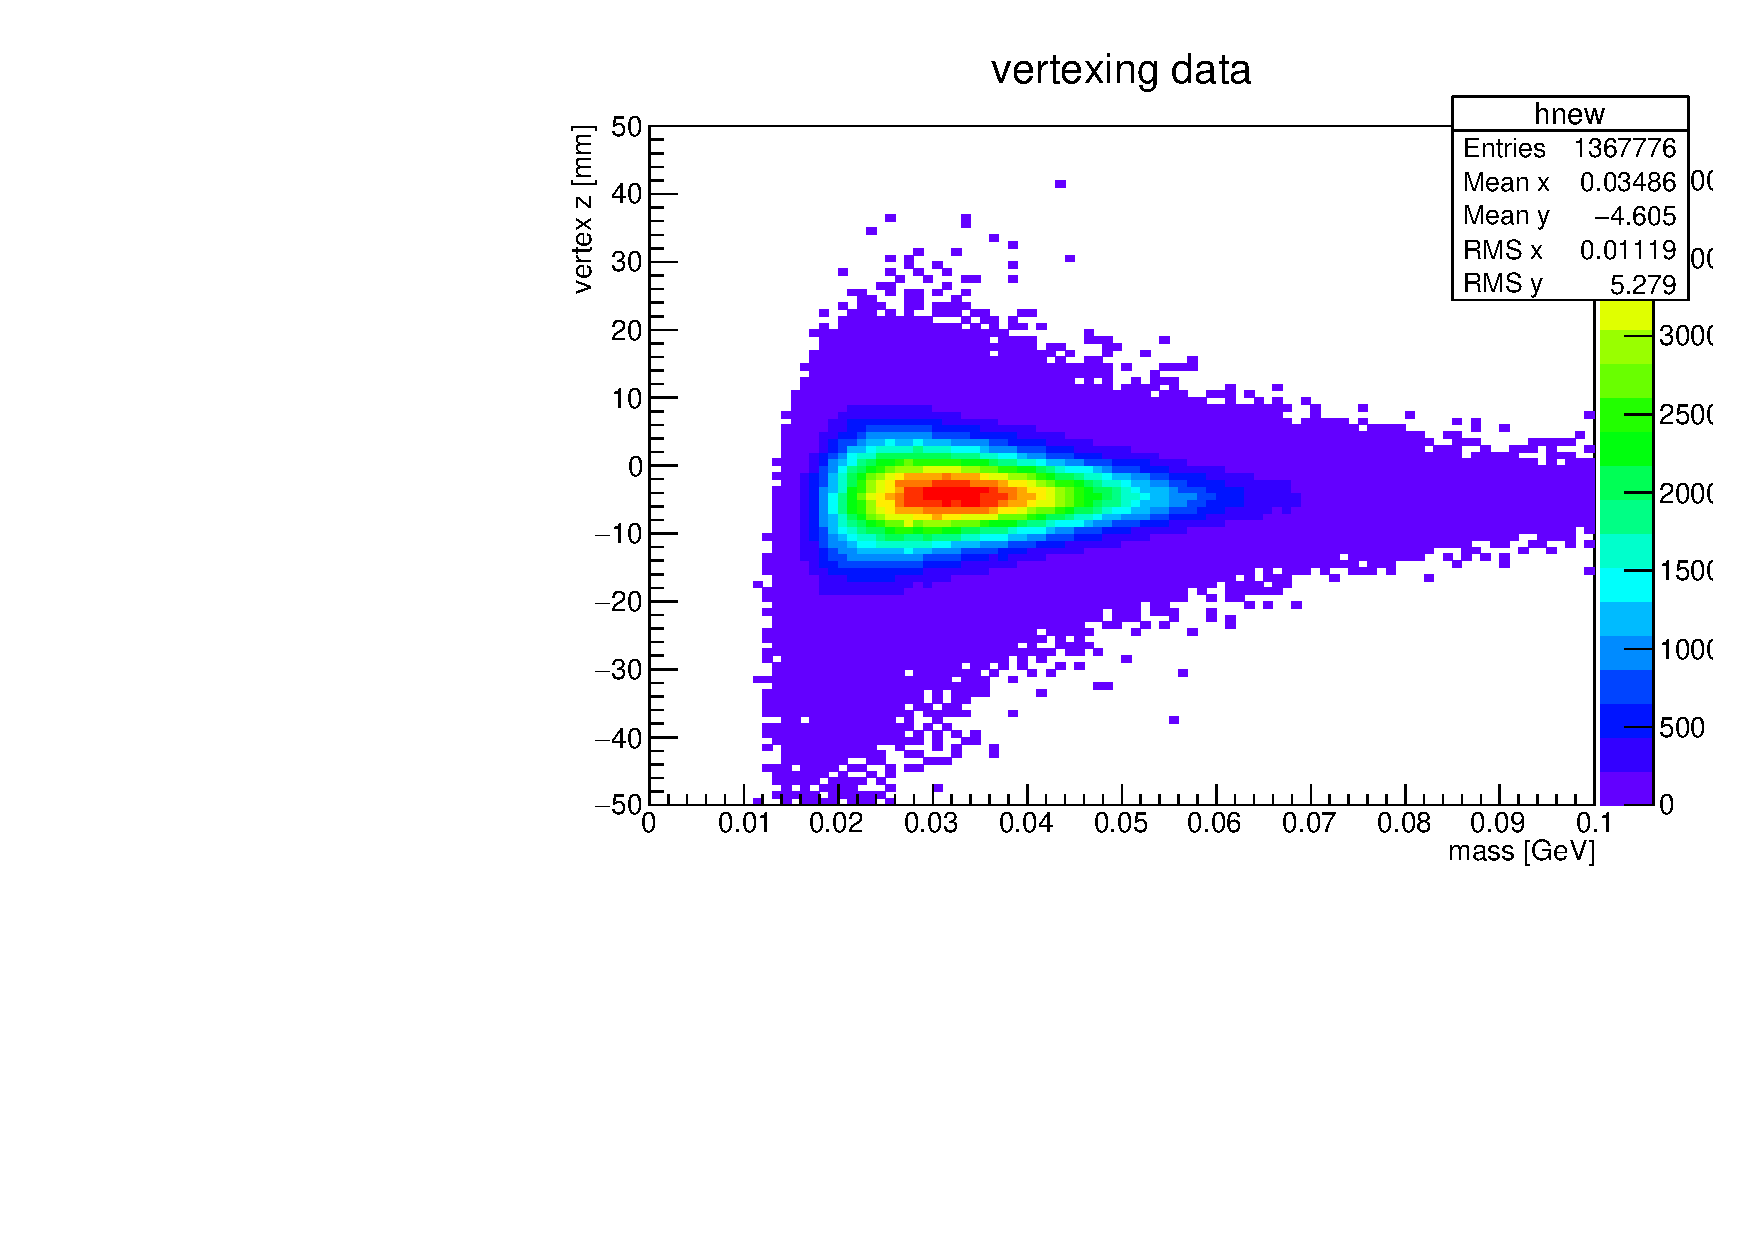
\includegraphics[width=0.7\textwidth,page=1,angle=-90]{vertexing/figs/golden_mres}
\end{center}
    \caption{Dataset for the vertexing analysis. The core of the vertex distribution is the horizontal band at $z=-5$ mm; a heavy photon signal would appear as a vertical band extending upwards from the core.}
    \label{fig:zvsmass}
\end{figure}

The pairs passing cuts are reduced to a 2-D dataset of points $(m,z)$, where each point is the mass $m$ and vertex location $z$ of a pair: see Figure \ref{fig:zvsmass}.
The vertex $z$ is defined relative to the nominal target position; as explained in Section \ref{sec:target_z}, the actual target position is at $z_{target}\approx -5$ mm.
To test for a heavy photon with $m_{A'}=m$, a resolution-limited mass slice is taken from the 2-D data set, and the vertex $z$ of the pairs in this mass slice are plotted as in Figure \ref{fig:vz_1d}.

\begin{figure}[ht]
\begin{center}
    \includegraphics[width=0.7\textwidth,page=61,angle=-90]{vertexing/figs/golden_mres}
\end{center}
\caption{Vertex $z$ (units of mm) for a resolution-limited mass slice (in data) centered at $m_{A'}=35.5$ MeV. A heavy photon signal would appear as a long rightwards tail (longer than the exponential fitted by the blue curve, which is the tail of the prompt vertex distribution).
    For this mass slice, $z_{cut}=26.6$ mm; there are four events with $z>z_{cut}$.}
    \label{fig:vz_1d}
\end{figure}

A cut is made at a minimum $z>z_{cut}$ to remove the large background from prompt $e^+e^-$ pairs.
$z_{cut}$ (plotted in Figure \ref{fig:zcut}) is set so the expected number of events past $z_{cut}$ is 0.5 according to a model of the prompt pairs distribution, described in Section \ref{sec:tails}.
This minimizes the prompt backgrounds and maximizes the heavy photon signal.
The rectangular region formed by the mass and $z$ cuts is the signal box for the heavy photon with mass $m_{A'}$.

If a heavy photon exists at some $m_{A'}$, heavy photon decays will appear in the data with a Gaussian mass distribution centered at $m_{A'}$, and a distribution of locations that extend from $z_{target}$ to positive $z$.
These events will appear in those mass slices that are close enough to $m_{A'}$ that they substantially overlap the Gaussian.

\begin{figure}[ht]
\begin{center}
    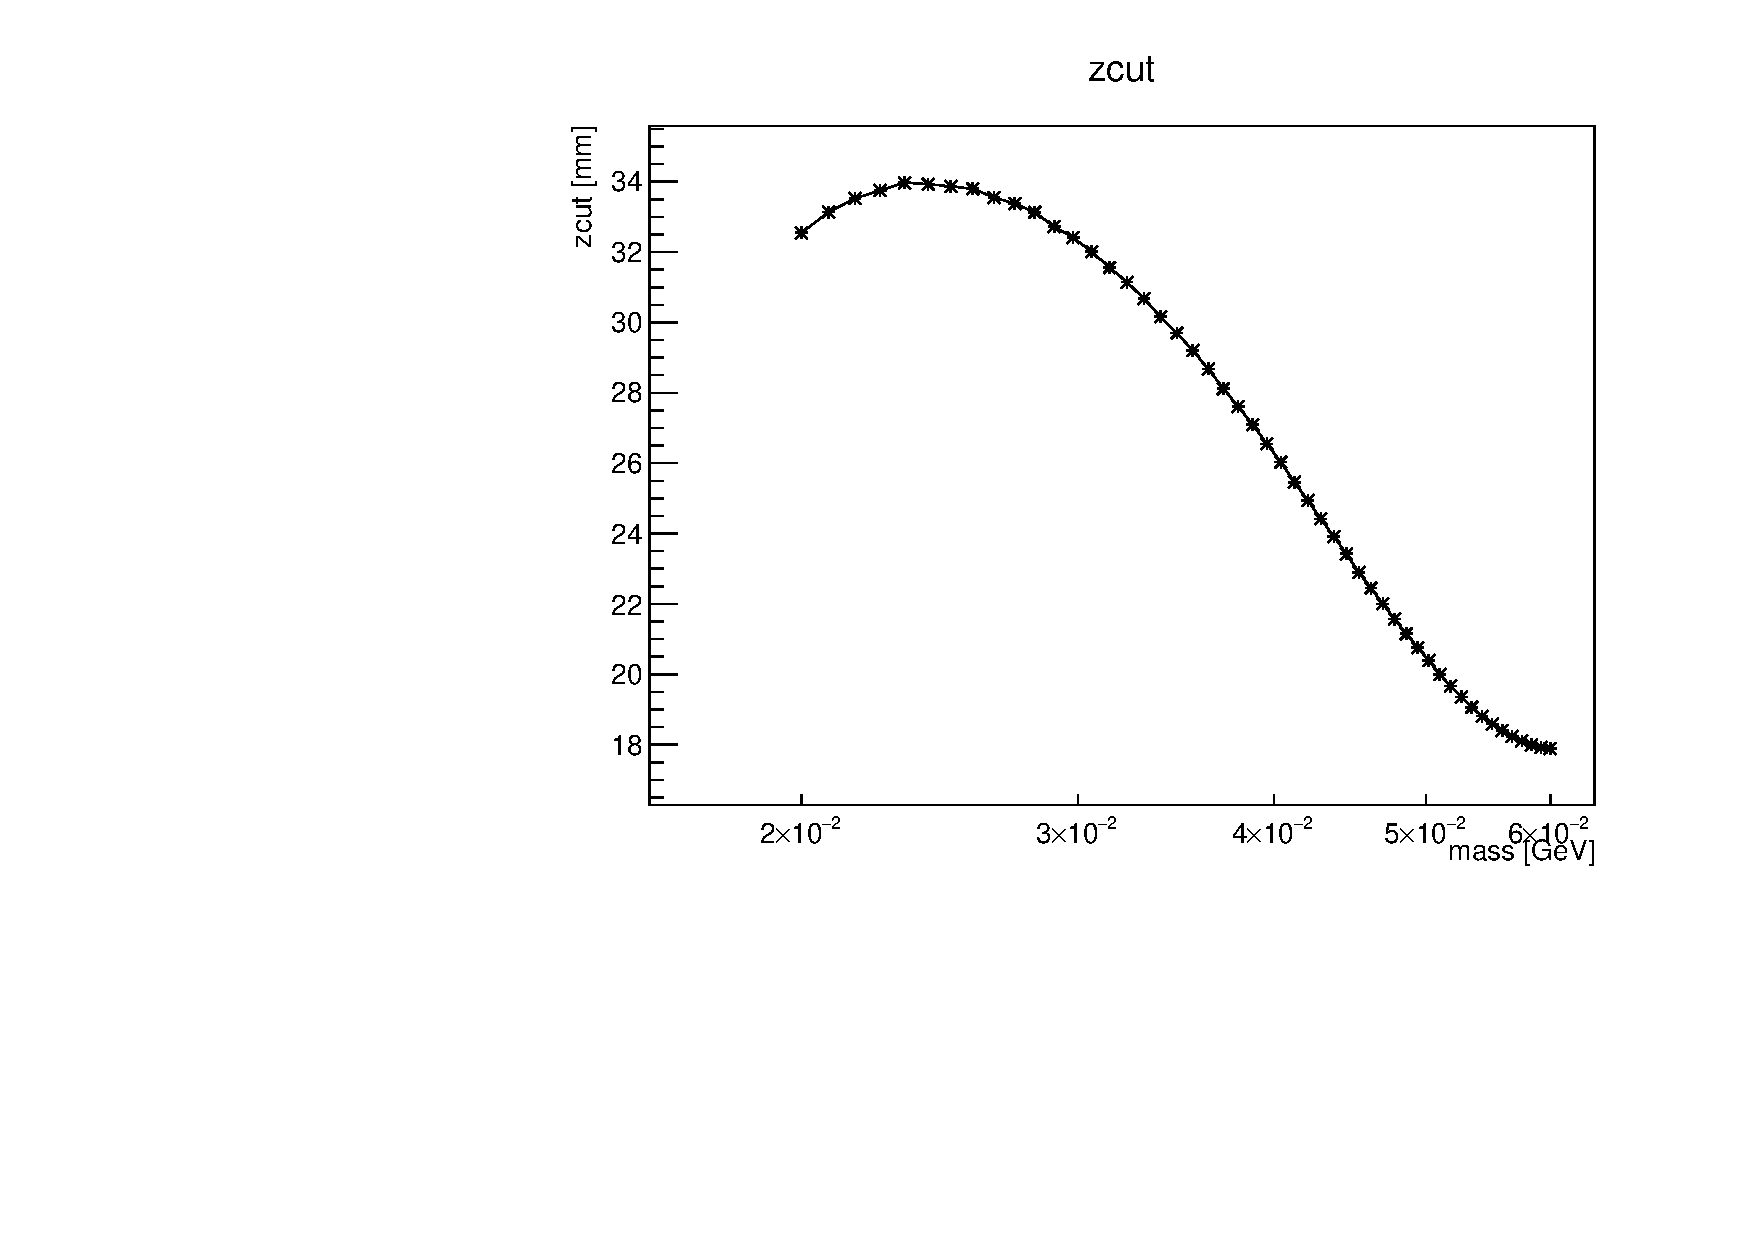
\includegraphics[width=0.7\textwidth,page=1,angle=-90]{vertexing/figs/golden_mres_output}
\end{center}
\caption{The value of the cut $z>z_{cut}$, as a function of the center of the mass slice.}
    \label{fig:zcut}
\end{figure}

Two types of analyses are performed on the data in the signal box.
The first is a cut-and-count analysis, where the number of pairs found in the signal box is compared to the number expected; this analysis gives the significance of any observed excess over background, and is described in Section \ref{sec:significance}.
The second analysis uses the optimum interval method to set an upper limit on the heavy photon production rate, and is described in Section \ref{sec:limits}.

\clearpage
\section{Monte Carlo Samples}
Simulated samples of all types of $e^+e^-$ pair events of interest (tridents, heavy photons, and wide-angle bremsstrahlung) are generated using MadGraph/MadEvent version 4 \cite{alwall_madgraph/madevent_2007}.
Beam backgrounds, such as elastically scattered electrons, that are created in the target and create pileup in the detector, are simulated using EGS5 \cite{hirayama_egs5_2005} and Geant4 \cite{agostinelli_geant4simulation_2003}.

\subsection{Trident and Wide-Angle Bremsstrahlung Monte Carlo}
\label{sec:tri_mc}
The trident processes (radiative and Bethe-Heitler tridents, as described in Section \ref{sec:physics_backgrounds}) are simulated using MadGraph/MadEvent.
One generator, called the ``full-diagram'' generator, incorporates all of the trident diagrams and their interference terms, and thus simulates (to lowest order) the combined rate of all $e^-Z\to e^+e^-e^-Z$.
%Both ``full-diagram'' and radiative tridents are simulated using MadGraph/MadEvent.
%The generator for full-diagram tridents includes radiative tridents, Bethe-Heitler tridents, and the interference terms.
Since radiative tridents are important for normalizing the heavy photon rate, a separate generator is used to generate radiative tridents on their own.

Wide-angle bremsstrahlung is the other important source of $e^+e^-$ pairs; as explained in Section \ref{sec:physics_backgrounds}, the primary electron and the positron from the pair conversion can fake an $e^+e^-$ pair.
MadGraph/MadEvent is used to produce $e^-\gamma$ events because it handles the angle correlations and the momentum transfer to the nucleus correctly.
The photon pair conversion is simulated in EGS5 (if in the target) or Geant4 (if in the SVT).

\subsection{Heavy Photon Monte Carlo}
\label{sec:ap_mc}
Heavy photon Monte Carlo samples are generated for values of $m_{A'}$ spaced out across the region of interest: 15, 16, 17, 18, 19, 20, 22, 24, 26, 28, 30, 35, 40, 50, 60, 70, 80, and 90 MeV.
The generator uses MadGraph/MadEvent, and fully simulates the momentum and angle spectra of the produced heavy photons.
In order to get complete coverage of $z>z_{target}$ for the purposes of the vertexing analysis, the decay vertices were displaced (in the direction of the heavy photon momentum, and accounting for variations in $\gamma$) according to an arbitrary decay length of $c\tau=1$ mm.

\clearpage
\section{Vertex Cuts}
\label{sec:vertex_cuts}
\begin{table}[ht]
    \begin{center}
        \caption{The full set of pair selection cuts for the vertexing analysis.
        Cuts carried over from the base selection are on top; cuts specific (or tightened) for vertexing are on bottom.}
        \begin{tabular}{lc}   
            \hline \hline
            Trigger type & ``pairs-1'' trigger \\
            Track-cluster matching (position) & $\chi^2_{match}<10$ \\
            Track-cluster matching (time) & $|t_{cl}-t_{trk}-43|<4$ ns \\
            Cluster time coincidence & $|t_{cl}(e^-)-t_{cl}(e^+)|<2$ ns \\
            Top-bottom requirement & $\sign(y_{cl}(e^-))\neq\sign(y_{cl}(e^-))$ \\
            Elastics cut & $p(e^-)<0.75E_{beam}$ \\
            Momentum sum cut & $p_{tot}(e^+e^-)<1.15E_{beam}$ \\
            Radiative cut & $p_{tot}(e^+e^-)>0.8E_{beam}$ \\
            \hline \hline
            Layer 1 requirement & layer 1 hits for both tracks \\
            Track quality & $\chi^2_{trk}<30$ \\
            Beamspot constraint & $\chi_{bsc}^2<10$, $\chi_{bsc}^2-\chi_{unc}^2<5$ \\
            Layer 1 isolation & see text \\
            Momentum asymmetry & $|p(e^-)-p(e^+)|/(p(e^-)+p(e^+))<0.4$ \\
            Positron DOCA & $d_0(e^+)<1.5$ mm \\
            \hline \hline
        \end{tabular}
        \label{tab:vertex_cuts} 
    \end{center}
\end{table}

Broadly speaking, there are three types of events that the vertexing cuts are meant to eliminate: layer 1 scatters, mishits, and wide-angle bremsstrahlung pairs.

Multiple scattering in layer 1 is the source of the Gaussian core of the vertex distribution, and also plays a role in the tails.
If one of the particles scatters in the first layer of the SVT, the track parameters at the vertex will be shifted.
The distribution of scattering angles is Gaussian at small angles where the scattering process is approximated by a random walk, but at large angles, the distribution is described by the Moli\`ere distribution, which approaches the power-law Rutherford scattering distribution.

Mishits happen when a particle scatters in the second (or later) layer of the SVT.
The scatter can shift the track so that a layer-1 hit from a different particle is more in line with the hits from layers 2 on; the track fit will then add the wrong hit to the track, and the track parameters at the vertex will be shifted.

The electron and positron of a wide-angle bremsstrahlung pair do not have the same origin: the electron comes from the bremsstrahlung interaction in the target, and the positron comes from a pair conversion that may happen in the target or in the SVT.
If the pair conversion happens in the SVT, the positron will not extrapolate to the target, and the reconstructed vertex may be pulled away from the target.
Because the positron is typically collinear with the photon, the effect on vertex $z$ is typically small, but these events are a identifiable component of the vertex distribution tails.

Figure \ref{fig:vertcut_performance} shows the effect of the vertex cuts on a mass slice in data. The efficiency for vertices near $z_{target}$ (presumed to be well-reconstructed) is roughly 60\%, and is similar for different masses.
The efficiency for displaced vertices (in Monte Carlo samples of heavy photons) is similar and does not degrade significantly with increasing $z$.
The individual cuts are described below.

\begin{figure}[ht]
\begin{center}
    \includegraphics[width=0.6\textwidth,page=2,angle=-90]{vertexing/figs/vertcutplots}
\end{center}
    \caption{Cumulative effect of the different vertex cuts on events in the mass slice centered at 30 MeV, passing base event selection cuts and meeting the layer 1 hit requirement.
    The tails at high $z$ are greatly reduced as cuts are applied (going from the black to the magenta distributions).
    }
    \label{fig:vertcut_performance}
\end{figure}

\subsection{Layer 1 Requirement}
\label{sec:layer1_cut}
The track reconstruction will find tracks with hits in any 5 out of the 6 layers.
This means that tracks can be reconstructed without layer 1 hits (as long as they have hits in all other layers).
Tracks without layer 1 hits have degraded mass and vertex resolution.
Furthermore, the tails of the vertex distribution extend to larger values of $z$.
For these reasons, it is not possible to use tracks with and without layer 1 hits as part of the same data set.

The background from wide-angle bremsstrahlung conversions is also significantly reduced by this cut.
In order to create charged tracks, the bremsstrahlung photon must convert in the target, either layer 1 sensor, or early enough in the upstream layer 2 sensor to make a hit there.
But in order to create charged tracks with layer 1 hits, the photon must convert in the target or the upstream layer 1 sensor.
The silicon sensors (0.35\% $X_0$) are significantly thicker than the portion of the target traversed by the average photon (half of 0.125\% $X_0$), so requiring that the track have a layer 1 hit cuts this background by roughly a factor of three.

The layer 1 requirement has a significant effect on the efficiency for long-lived, low-mass heavy photons.
As seen from the target, all layers of the SVT have their inner edges at $\pm 15$ mrad vertical angle from the beam plane.
As seen by a heavy photon decaying downstream of the target, layer 1 is at a significantly larger vertical angle than the others, and so the minimum $m_{A'}$ needed to hit layer 1 is larger.
Put another way, this means that the maximum $z$ for detecting a heavy photon of given $m_{A'}$ is smaller if layer 1 is required; this is shown in Figure \ref{fig:eff_z_alllayers}.
The impact of this effect is discussed in Section \ref{sec:reach_projections}.

\begin{figure}[ht]
\begin{center}
    \includegraphics[width=0.35\textwidth,page=7,angle=-90]{vertexing/figs/acceptance_data}
    \includegraphics[width=0.35\textwidth,page=7,angle=-90]{vertexing/figs/acceptance_alllayers_data}
\end{center}
\caption{Efficiency curves for $m_{A'}=40$ MeV. Left: requiring layer 1 hits for both tracks. Right: full HPS acceptance.}
    \label{fig:eff_z_alllayers}
\end{figure}

\subsection{Track Quality}
As explained in Section \ref{sec:event_selection}, the track $\chi^2$ is not a very selective cut when studied as part of the base event selection (where the objective is to reject accidental coincidences).
However, poor track fits can lead to poor vertex fits, and so events with poor track $\chi^2$ do contribute to the tails of the vertex $z$ distribution.
This is shown in Figure \ref{fig:trkchisq_performance}.

\begin{figure}[ht]
\begin{center}
    \includegraphics[width=0.6\textwidth,page=3,angle=-90]{vertexing/figs/vertcutplots}
\end{center}
    \caption{Effect of the track quality cut on events in the mass slice centered at 30 MeV, and passing all other cuts.
%    The $z$ distributions of events rejected by these cuts have longer tails, so these cuts 
    }
    \label{fig:trkchisq_performance}
\end{figure}

\subsection{Beamspot Constraint}
The beamspot constraint uses the vertex fit to identify the common situation where one track points back to the beamspot at the target as it should, but the other does not.
If the second track (due to scattering, mishits or any other effect) intersects the beam axis downstream of the target, the reconstructed vertex will be pulled downstream along the first track.
The effect is that the reconstructed $z$ will be pulled downstream of the target, but the reconstructed vertex $y$ is also pulled up or down in a way that is inconsistent with a true displaced decay.
The beamspot constraint is meant to identify these inconsistencies.

As explained in Section \ref{sec:vertex_recon}, the vertex reconstruction can use a ``beamspot-constrained'' fit where the vertex momentum is required to point back to the beamspot at $z_{target}$.
The $\chi^2$ of this vertex fit is the sum of two factors: the consistency of the vertex (how close the tracks are to intersecting each other) and the consistency with the beamspot constraint (how close the vertex is to pointing back to the beamspot).
The ``unconstrained'' vertex fit $\chi^2$ contains only the first factor.

Cuts are applied on both the beamspot-constrained vertex $\chi^2$ and the difference between the beamspot-constrained and unconstrained vertex $\chi^2$.
The effect of these cuts is shown in Figure \ref{fig:bsc_performance}.

\begin{figure}[ht]
\begin{center}
    \includegraphics[width=0.6\textwidth,page=4,angle=-90]{vertexing/figs/vertcutplots}
\end{center}
    \caption{Effect of the beamspot constraint cuts on events in the mass slice centered at 30 MeV, and passing all other cuts.
%    The $z$ distributions of events rejected by these cuts have longer tails, so these cuts 
    }
    \label{fig:bsc_performance}
\end{figure}

\subsection{Isolation Cut}
The isolation cut rejects possible mishits by looking at the other hits in layer 1 of the SVT.
If a mishit on a track pulls the vertex downstream, the real hit from the particle will be close to the hit that was mistakenly associated with the track, but further away from the beam plane.
Since the track parameters at the vertex are most strongly determined by the layer 1 and layer 2 hits, and the lever arm from the target to layer 2 is twice that from layer 1 to layer 2, typically the track $y$ at the target will shift by double the distance between the real hit and the mishit.
This geometry is illustrated in Figure \ref{fig:isolation_schematic}.

\begin{figure}[ht]
\begin{center}
    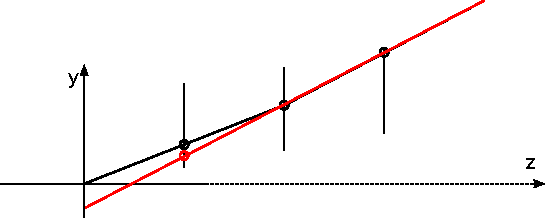
\includegraphics[width=0.6\textwidth]{vertexing/figs/isolation}
\end{center}
    \caption{Illustration of a track with a mishit.
    This view shows the Z (beam direction, beam travels left to right) and Y (magnetic field direction) axes, and three SVT layers with hits (circles).
    The true particle trajectory (black) starts at the target, is scattered at layer 2, and continues on to layer 3.
    Because the true trajectory is not straight, a better track fit can be made using a hit (red circle) from a different particle.
    The resulting track fit (red line) misses the target and, if used in a vertex fit, will lead to a best-fit vertex downstream of the target.
    }
    \label{fig:isolation_schematic}
\end{figure}

Therefore an ``isolation'' value is calculated for each of the layer 1 hits, as the distance to the closest hit in the outwards direction.
If the isolation is less than 0.5 times the track's distance of closest approach to the beamspot in the $y-z$ plane, the hit on the track may be a mishit and the closest hit might be the real hit.
If this is the case for any of the four isolations (one for each layer 1 sensor), the pair is rejected.
The effect of this cut is shown in Figure \ref{fig:isolation_performance}.

\begin{figure}[ht]
\begin{center}
    \includegraphics[width=0.6\textwidth,page=5,angle=-90]{vertexing/figs/vertcutplots}
\end{center}
    \caption{Effect of the isolation cut on events in the mass slice centered at 30 MeV, and passing all other cuts.
    By design the isolation cut has little impact on vertices with $z\approx z_{target}$, since the tracks in those pairs pass close to the beamspot.
    }
    \label{fig:isolation_performance}
\end{figure}

\subsection{Momentum Asymmetry and Positron DOCA}
Two cuts are meant to reject wide-angle bremsstrahlung pairs.

Because the electron from a bremsstrahlung interaction typically carries more momentum than the photon, the electron in a WAB pair usually has higher momentum than the positron.
Heavy photons and radiative tridents have a symmetric distribution of electron and positron momentum, so a cut is used to reject pairs where the electron has much higher momentum than the positron.

If the pair conversion happens in the SVT, the positron track will curve wide of the target since the positron is roughly collinear with the photon, which does not bend in the magnetic field.
This appears in the track parameters as a positive DOCA (distance of closest approach) in the X-Z plane.
Therefore, pairs with large positive positron DOCA are rejected.

\begin{figure}[ht]
\begin{center}
    \includegraphics[width=0.35\textwidth,page=6,angle=-90]{vertexing/figs/vertcutplots}
    \includegraphics[width=0.35\textwidth,page=7,angle=-90]{vertexing/figs/vertcutplots}
\end{center}
    \caption{Effect of the WAB rejection cuts on events in the mass slice centered at 30 MeV, and passing all other cuts.
    The $z$ distributions of events rejected by these cuts are wider than the events that pass, showing that while wide-angle bremsstrahlung conversions do not have systematic shifts in vertex $z$, they contribute to the tails of the $z$ distribution.
    }
    \label{fig:wabcut_performance}
\end{figure}

\subsection{Tuning Cuts}
Data is used to tune the cuts to keep pairs with $z$ close to $z_{target}$, and reject pairs with large positive $z$.
In general, tuning cuts on the data can introduce bias.
In this case, only the unblinded 10\% of the full dataset is being used (and will be used, even after the data is unblinded) for tuning cuts; even if a heavy photon is present in the tuning data, the number of expected events is negligible.
Also, since the cuts are not tuned for individual mass slices, any possible heavy photon signal will not be as prominent in the tuning process as it would be in the analysis.

Heavy photon Monte Carlo is used to check that none of the cuts have an unexpected adverse effect on efficiency for displaced vertices.

\clearpage
\section{Fit Inputs}

%The events passing cuts are reduced to a 2-D dataset of points $(m,z)$, where each point is the mass $m$ and vertex Z-coordinate $z$ of an event.

To test for a heavy photon at mass $m_{A'}$ and coupling $\epsilon^2$, the signal, background, and resolutions must be modeled as inputs to the analyses.

The mass cut is set to keep only events with $|m-m_{A'}|<1.4 \sigma_m(m_{A'},z)$, where $\sigma_m$ is the mass resolution expected for heavy photons with mass $m_{A'}$.
The mass resolution depends on the mass and the vertex position, and is estimated using Monte Carlo: this is explained in Section \ref{sec:mres}.
This mass window is chosen to accept a large fraction of the signal events, without accepting too many background events.
A window of $\pm1.4\sigma$ (which accepts 83.8\% of the signal events) optimizes significance for high-statistics, high-background experiments where significance is proportional to $S/\sqrt{B}$.
The optimality of this window is not exact for low statistics (where the Poisson distribution cannot be safely approximated as a Gaussian), but is still approximately true.

After cutting on $m$, the dataset is reduced to one dimension.
An additional cut is made to keep only events with $z>z_{cut}$, rejecting the region where the background strongly dominates and there is no sensitivity to a signal.
$z_{cut}$ is chosen such that only 0.5 events are expected past $z=z_{cut}$, based on the fitted shape of the background distribution.
The amplitude of the background distribution is taken from the peak of the vertex distribution; the shape is taken from Monte Carlo as described in Section \ref{sec:tails}.

Setting limits requires knowledge of the expected signal distribution, $S(z;m_{A'},\epsilon^2)$.
This is described in Section \ref{sec:signal_shape}.

\clearpage
\subsection{Estimating the Mass Resolution}
\label{sec:mres}

The mass resolution $\sigma_m$ for a $e^+e^-$ pair depends on the momentum resolutions $\sigma_{p_{e^+}},\sigma_{p_{e^-}}$ for the two particles, the resolution $\sigma_\theta$ of the opening angle, and their covariances.
Since the opening angle and momentum measurements predominantly rely on different parts of the SVT (opening angle on the upstream half of the SVT, momentum on the downstream half), their covariance is negligible.
Neglecting the electron mass, and using the small-angle approximation for the opening angle,
\begin{equation}
m=\sqrt{(1-\cos\theta)p_{e^+}p_{e^-}} \approx \frac{1}{\sqrt{2}}\theta\sqrt{p_{e^+}p_{e^-}}
\end{equation}
\begin{equation}
\sigma_m\approx \frac{1}{\sqrt{2}}\left(\theta \frac{\sqrt{p_{e^+}p_{e^-}}}{2}\left(\frac{\sigma_{p_{e^+}}}{p_{e^+}}+\frac{\sigma_{p_{e^-}}}{p_{e^-}}\right)  + \sigma_\theta\sqrt{p_{e^+}p_{e^-}} \right)
%\sigma_m\approx \frac{1}{\sqrt{2}}(\theta\sigma_{\sqrt{p_{e^+}p_{e^-}}} + \sigma_\theta\sqrt{p_{e^+}p_{e^-}})
\end{equation}
$\theta$ is the only term in this expression with a strong dependence on $m$ or $z$: it is proportional to $m$.
Because the momentum resolution is dominated by multiple scattering, the fractional momentum resolutions $\frac{\sigma_{p_{e^+}}}{p_{e^+}}$ and $\frac{\sigma_{p_{e^-}}}{p_{e^-}}$ do not depend strongly on the momentum; nor do they depend on the track angles.
The opening angle resolution is determined by the resolutions for the two track slopes, which do not depend strongly on the track slopes, so $\sigma_\theta$ is roughly constant.
The conclusion is that $\sigma_m$ is expected to depend linearly on $m$, and not at all on $z$.

Mass resolution is measured using the Monte Carlo samples of reconstructed heavy photons described in Section \ref{sec:ap_mc}.
For each $m_{A'}$, the residual between the reconstructed mass and true mass is plotted against the true $z$.
The width of the residual distribution at each $z$ is fitted with a Gaussian to get the mass resolution at that $z$, $\sigma_m(m_{A'},z)$.
The mass resolution is fitted with a first-order polynomial in $z$:
$\sigma_m(m_{A'},z) = a_0(m_{A'}) + a_1(m_{A'}) z$.
Then the polynomial coefficients are themselves fitted with first-degree polynomials in $m_{A'}$: $a_0(m_{A'}) = a_{00} + a_{01}m_{A'}$, $a_1(m_{A'}) = a_{10} + a_{11}m_{A'}$.
The result of this procedure is a model for the mass resolution: $\sigma_m(m_{A'},z) = (a_{00} + a_{01}m_{A'}) + (a_{10} + a_{11}m_{A'}) z$.

%However $\sigma_m$ increases with $z$ as shown in Figure \ref{fig:skewed_mres}, and $a_{11}$ is significantly positive.
%This seems to be an effect of a bug in the vertex fitter, which does not correctly calculate the opening angle at the vertex.
%The reconstructed mass has a systematic dependence on the opening angle in the X-Z plane, which widens the distribution of reconstructed masses as shown in Figure \ref{fig:mass_skew}.
%If this effect is subtracted out, the mass resolution becomes constant with respect to $z$, as shown in Figure \ref{fig:fixed_mres}.

%\begin{figure}[ht]
%\begin{center}
    %\includegraphics[width=0.7\textwidth,page=4,angle=-90]{vertexing/figs/acceptance_40}
%\end{center}
    %\caption{Mass resolution vs. $z$ for 40 MeV heavy photons. The resolution gets worse with increasing $z$.}
    %\label{fig:skewed_mres}
%\end{figure}

%\begin{figure}[ht]
%\begin{center}
    %\includegraphics[width=0.7\textwidth,page=5,angle=-90]{vertexing/figs/acceptance_40}
%\end{center}
    %\caption{Mass resolution for 40 MeV heavy photons decaying near $z=30$ mm. The mass residual has a systematic dependence on the opening angle in the X-Z plane.}
    %\label{fig:mass_skew}
%\end{figure}

\begin{figure}[ht]
\begin{center}
    \includegraphics[width=0.7\textwidth,page=5,angle=-90]{vertexing/figs/acceptance_30}
\end{center}
    \caption{Mass resolution vs. $z$ for 40 MeV heavy photons in Monte Carlo.
    Top: mass residual (difference between the reconstructed mass and the true mass) vs. $z$ for 40 MeV heavy photons.
    Bottom: the widths of Gaussian fits to vertical slices of the top distribution (blue points), and a linear fit to the points (red line).
    The slope of the linear fit is consistent with 0, showing that the mass resolution is constant with respect to $z$.}
    \label{fig:fixed_mres}
\end{figure}

The fitted values of $a_{10}$ and $a_{11}$ are consistent with 0, as expected.
After this procedure, this is the mass resolution model (including statistical uncertainties in the last digits of the coefficients):
\begin{equation}
\sigma_m(m_{A'},z) = 0.00072(2) \mathrm{GeV} + 0.0382(4) m_{A'}
\end{equation}

\begin{figure}[ht]
\begin{center}
    \includegraphics[width=0.7\textwidth,page=12,angle=-90]{vertexing/figs/acceptance_data}
\end{center}
\caption{Mass resolution vs. $m_{A'}$. The blue marker is the M{\o}ller mass resolution in data.}
    \label{fig:mres_data}
\end{figure}

M{\o}ller scattering is one check of the mass resolution.
As explained in Section \ref{sec:mollers}, pairs of electrons from M{\o}ller scattering have a fixed invariant mass equal to the center-of-mass energy.
The width of the M{\o}ller mass distribution is therefore a useful check.
Figure \ref{fig:moller_mres} shows the M{\o}ller mass distribution in data, which has $\sigma_m=2.168$ MeV.
As shown in Figure \ref{fig:mres_data}, this is within 10\% of the heavy photon mass resolution from Monte Carlo (1.973 MeV).
The difference between data and Monte Carlo resolutions is believed to be due to the incomplete SVT alignment, for which work is still in progress.

\begin{figure}[ht]
\begin{center}
    \includegraphics[width=0.7\textwidth,page=17,angle=-90]{vertexing/figs/mollerplots}
\end{center}
    \caption{Distribution of reconstructed invariant mass of M{\o}ller pairs, with a Crystal Ball fit showing the mass resolution.}
    \label{fig:moller_mres}
\end{figure}

\clearpage
\subsection{Estimating the Signal Distribution}
\label{sec:signal_shape}
The expected distribution of signal events can be expressed as $\mu_{exp} s(z)$, where $\mu_{exp}$ is the expected number of reconstructed heavy photon events after the mass and $z$ cuts, and $s(z)$ is the probability density function (normalized to unit integral) of the $z$ locations.
The distribution is estimated as the following product of terms, where each term can depend on $m_{A'}$ and $\epsilon^2$:
\begin{equation}
\mu_{exp} s(z) = (N_{A'}\epsilon_{reco}(z_{target}))\frac{e^{\frac{z_{target}-z}{\gamma c \tau}}}{\gamma c \tau}\frac{\epsilon_{reco}(z)}{\epsilon_{reco}(z_{target})} \epsilon_{cut}(z)
\end{equation}
$N_{A'}$ is the number of heavy photons produced in the target.
The exponential function is the distribution of decays along $z$, and is normalized to 1.
$\epsilon_{reco}(z)$ is the efficiency to detect and reconstruct an $e^+e^-$ pair produced at a given $z$.
$\epsilon_{cut}(z)$ is the efficiency of the mass and $z$ cuts for a heavy photon with mass $m_{A'}$ decaying at a given $z$. It equals 0 for $z<z_{cut}$, and 0.838 for $z\ge z_{cut}$.

In principle, this distribution should be smeared by $\sigma_z$, the resolution of the vertex position: this is not done since the signal distribution varies slowly on the scale of $\sigma_z$ (which is 3-6 mm, depending on $m$).

\subsubsection{Production Rate and Radiative Fraction}

$N_{A'}\epsilon_{reco}(z_{target})$ is estimated using data and Equation \ref{eq:production}, which shows that $N_{A'}$ is linked to $\frac{\mathrm{d}N_{rad}}{\mathrm{d}m}$, the number of radiative tridents produced with masses around $m_{A'}$.
The data gives $\frac{\mathrm{d}N_{e^+e^-}}{\mathrm{d}m}\epsilon_{reco}(z_{target})$, the number of $e^+e^-$ pairs produced and detected in a mass window around $m_{A'}$; some fraction of these are radiative tridents.
The fraction is estimated using Monte Carlo.

The Monte Carlo samples described in Section \ref{sec:tri_mc} are used to calculate the normalized cross-sections (after detector and reconstruction efficiencies, and all cuts) for radiative tridents only, for all tridents, and for wide-angle bremsstrahlung conversions.
The radiative trident fraction is the ratio of the cross-section for radiative tridents to the total cross-section for $e^+e^-$ pairs.

\begin{figure}[ht]
\begin{center}
    \includegraphics[width=0.35\textwidth,page=5,angle=-90]{vertexing/figs/frac}
    \includegraphics[width=0.35\textwidth,page=6,angle=-90]{vertexing/figs/frac}
\end{center}
    \caption{Left: rates of processes producing $e^+e^-$ pairs, with the sum in black. Right: the radiative fraction, which is calculated by dividing the black histogram by the red histogram.}
    \label{fig:radfrac}
\end{figure}

\subsubsection{Decay Length}
The decay length is calculated using Equation \ref{eq:lifetime}, which gives the lifetime $\tau$ for a given $m_{A'}$ and $\epsilon^2$.
The boost $\gamma$ equals $E_{beam}/m_{A'}$ if the heavy photon takes the full beam energy, but this is not completely accurate; in reality the average boost is slightly less than the maximum.

Monte Carlo samples are used to find the correct distribution of decay lengths.
The decay $z$ is plotted for an MC sample of heavy photons with mass $m_{A'}$ and an arbitrary lifetime, with the requirement that the heavy photon momentum be at least $0.8E_{beam}$ (matching the analysis cut), and fit with an exponential.
The decay constant of the exponential is compared to the $\gamma c \tau$ that would be expected from $\gamma=E_{beam}/m_{A'}$; this shows that the typical $\gamma$ is roughly $0.95E_{beam}/m_{A'}$.

\begin{figure}[ht]
\begin{center}
    \includegraphics[width=0.7\textwidth,page=1,angle=-90]{vertexing/figs/acceptance_40}
\end{center}
    \caption{Top: distribution of decay $z$ for heavy photons ($m_{A'}=40$ MeV, $c\tau=1$ mm) carrying at least 80\% of the beam momentum. Bottom: the momentum distribution for the heavy photons.}
    \label{fig:decay_z_truth}
\end{figure}

\subsubsection{Efficiency}
\label{sec:efficiency_z}

The efficiency $\epsilon_{reco}$ for reconstructing a heavy photon decay depends on $m_{A'}$ and the decay $z$.
The measurement of the radiative trident rate implicitly includes a factor of $\epsilon_{reco}(m_{A'},z_{target})$, so Monte Carlo is only needed to estimate $\frac{\epsilon_{reco}(m_{A'},z)}{\epsilon_{reco}(m_{A'},z_{target})}$, the efficiency falloff as a function of vertex displacement.
This assumes that any detector-based inefficiencies not represented in the Monte Carlo are independent of $z$.

The efficiency falls off with $z$ because the further downstream the decay, the larger the opening angle in the Y-Z plane necessary to hit layer 1 of the SVT.
At some cutoff value of $z$ it is no longer possible for both the electron and the positron to hit layer 1; the efficiency starts to fall off well before that cutoff.
This effect is more severe for lower $m_{A'}$, where the opening angle is smaller.

The efficiency is measured using the Monte Carlo samples of generated and reconstructed heavy photons described in Section \ref{sec:ap_mc}.
For each $m_{A'}$, the distribution of decay $z$ is filled both for generated and reconstructed heavy photons.
The ratio of the two distributions gives $\epsilon_{reco}(m_{A'},z)$.
This is scaled so it equals 1 at $z=z_{target}$, and is fitted with a function of the form $\frac{\epsilon_{reco}(m_{A'},z)}{\epsilon_{reco}(m_{A'},z_{target})} \approx \exp(p_3 z^3 + p_2 z^2 + p_1 z + p_0)$.
The parameters $p_3$, $p_2$, $p_1$, and $p_0$ are fit with polynomials in $m_{A'}$: $p_0$ and $p_1$ are fit with first-order polynomials, and $p_2$ and $p_3$ are fit with third-order polynomials.

\begin{figure}[ht]
\begin{center}
    \includegraphics[width=0.7\textwidth,page=2,angle=-90]{vertexing/figs/acceptance_40}
\end{center}
    \caption{Top: distribution of decay $z$ for reconstructed heavy photons ($m_{A'}=40$ MeV, $c\tau=1$ mm). Bottom: efficiency curve $\frac{\epsilon_{reco}(m_{A'},z)}{\epsilon_{reco}(m_{A'},z_{target})}$, with fit.}
    \label{fig:eff_z}
\end{figure}

\clearpage
\subsection{Fitting the Background Distribution}
\label{sec:tails}
The background distribution consists of a Gaussian core and a non-Gaussian tail.
The width of the Gaussian core is set by multiple scattering and is well understood, but the tails extend much farther than the Gaussian.
For $z>z_{cut}$, the background distribution is dominated by the tails: $z_{cut}$ is typically at least $5\sigma_z$.

The background distribution is estimated from Monte Carlo.
This is necessary because if the background distribution were fit from the data, and there is actually a heavy photon signal in the data, the fit would be pulled so as to understate the size of the signal.
As in Figure \ref{fig:vertex_data-mc}, comparisons of the background distribution in Monte Carlo and data show that the Monte Carlo accurately simulates the processes that control the vertex resolution: the resolution in the Gaussian core and tails found in Monte Carlo are good fits to the data.

\begin{figure}[ht]
\begin{center}
    \includegraphics[width=0.7\textwidth]{vertexing/figs/slice-36}
\end{center}
\caption{Comparison of vertex Z distributions between data (black) and Monte Carlo (red).}
    \label{fig:vertex_data-mc}
\end{figure}

The 2-dimensional vertex distribution from Monte Carlo is scanned in $m$, using the same mass cut that is used for the analysis.

The background distribution is fit with a 4-parameter piecewise function defined from a Gaussian and an exponential.
The Gaussian is defined with the usual parameters of mean $\bar{z}$ and standard deviation $\sigma$.
The parameter $b$ defines the distance from the Gaussian's mean where the distribution transitions to the exponential.
The exponential is defined in terms of a tail length $l$, and its amplitude is fixed by the requirement that the function be continuous.
This function is similar to the ``GaussExp'' function described in \cite{cms_collaboration_search_2015}, except GaussExp fixes the exponential's decay length by requiring that the function be continuously differentiable.
\begin{equation}
B(z;\bar{z},\sigma,b,l)=
\begin{cases}
e^{-\frac{(z-\bar{z})^2}{2\sigma^2}} &\text{if } z\le\bar{z}+b,\\
e^{-\frac{b^2}{2\sigma^2} - (z-\bar{z}-b)/l}  &\text{if } z\ge\bar{z}+b
\end{cases}
\label{eq:gaussexp}
\end{equation}

\begin{figure}[ht]
\begin{center}
    \includegraphics[width=0.7\textwidth,page=61,angle=-90]{vertexing/figs/golden_mres}
\end{center}
\caption{Vertex $z$ (units of mm) for a mass slice in data, with the background model in blue.}
    \label{fig:vz_fit}
\end{figure}

The values of $b$ and $l$ found at each $m_{A'}$ are fitted to cubic polynomials in $m_{A'}$.
When estimating $B(z)$ for data, the values of $b$ and $l$ are fixed to the values found for Monte Carlo, but the Gaussian parameters are allowed to float.

\subsubsection{Characterizing Excess Backgrounds}
\label{sec:excess_background}
If the tails of the vertex distribution are completely described by the exponential tail of the background model of Equation \ref{eq:gaussexp}, each mass slice should by construction (on average, and in the absence of a possible heavy photon signal) contain 0.5 events with $z>z_{cut}$.
But as seen in Figure \ref{fig:n_candidates}, most mass slices contain more than one event with $z>z_{cut}$, and some contain as many as 4 events; this is a significant excess.
This indicates either that there is a heavy photon in the data, or that there is a background not described by the background model.

\begin{figure}[ht]
\begin{center}
    \includegraphics[width=0.7\textwidth,page=8,angle=-90]{vertexing/figs/golden_mres_output}
\end{center}
\caption{Number of events found with $z>z_{cut}$ in each mass slice, as a function of the center mass of the mass slice.
If the background model fully describes the data, the mean number per mass slice of events with $z>z_{cut}$ should be 0.5.}
    \label{fig:n_candidates}
\end{figure}

\begin{figure}[ht]
\begin{center}
    \includegraphics[width=0.7\textwidth,page=4,angle=-90]{vertexing/figs/golden_mres_output}
\end{center}
\caption{The set of events that appear with $z>z_{cut}$ in at least one mass slice.
This is the same histogram as Figure \ref{fig:zvsmass}, but only plotting events above $z=z_{cut}$ (the black curve).
Some events are close to $z=z_{cut}$, but some events are substantially above the black line ($z\gg z_{cut}$).}
    \label{fig:zvsmass_candidates}
\end{figure}

The events with $z>z_{cut}$ can be characterized by their distributions in $z$ and in mass.
Events consistent with the background model should have $z$ close to $z_{cut}$ (the median $z-z_{cut}$ is proportional to $l$), but be uniformly distributed, with an average of 0.5 events per mass slice.
Any other component of the background might have a different distribution in $z$, but will be broadly distributed in mass.
Events from heavy photon decays should have large $z$ and a tight distribution in mass (limited by the mass resolution).

If the excess events are described by the background model, the events with $z>z_{cut}$ in a mass slice should be distributed according to the exponential distribution.
Transforming by the cumulative distribution function of the exponential, $z\to 1-e^{(z_{cut}-z)/l}$, gives the quantile of each event in the background model; if the background model describes the events, the quantiles should be distributed uniformly.
Some of the events with $z>z_{cut}$ do appear to follow this pattern, but some have large quantiles, meaning that they have $z$ larger than would be typical from sampling the background model.

\begin{figure}[ht]
\begin{center}
    \includegraphics[width=0.6\textwidth,page=60,angle=-90]{vertexing/figs/golden_mres}
\end{center}
\caption{The background CDF values (quantiles) for events in the mass slice centered at $m_{A'}=35.6$ MeV that have $z>z_{cut}$ (this is the same mass slice as Figure \ref{fig:vz_1d}).
The two events with $z\approx 35$ have quantiles close to 1, suggesting that their values of $z$ are larger than would be expected from the background model.}
    \label{fig:candidates_rescaled}
\end{figure}

\begin{figure}[ht]
\begin{center}
    \includegraphics[width=0.7\textwidth,page=7,angle=-90]{vertexing/figs/golden_mres_output}
\end{center}
\caption{The background quantiles for events that have $z>z_{cut}$ in each mass slice.
This is not a true histogram; each vertical column is a histogram similar to Figure \ref{fig:candidates_rescaled}, but a given event is plotted in every mass slice where it appears.
The quantile for a given event changes with the mass slice because $z_{cut}$ depends on the mass slice.
}
    \label{fig:zvsmass_candidates_rescaled}
\end{figure}

If we (somewhat arbitrarily) separate the two sets of events by cutting at a quantile of 0.9, the events with low quantiles contribute 0.52 events per mass slice; this suggests that these events are consistent with the background model and occur with the correct frequency, but the high-$z$ events with quantiles above 0.9 are in excess of the expected background.
These are the five events on the upper right of Figure \ref{fig:zvsmass_candidates}.

The five events isolated by the quantile cut are spread broadly in mass: their RMS in mass is 4.2 MeV, much larger than the estimated mass resolution (2.2 MeV) at the mean mass (38.2 MeV).
No mass slice captures more than three of these events; if all five events were decays of a heavy photon at a single $m_{A'}$, the lowest- and highest-mass events would be deviations of more than $2\sigma_m$ from $m_{A'}$.
These events do not match the signature of a heavy photon.

The rate of these events is also not consistent with a heavy photon, or with beam-gas interactions.
The expected number of heavy photon decays in this data is much less than 1, as discussed in \ref{sec:results}.
Beam-gas interactions, where beam electrons interact with residual gas in the beamline to create $e^+e^-$ pairs downstream of the target, are another potential source of displaced vertices, but cannot explain these events.
The beamline vacuum was measured to be in the $10^{-5}$ torr range, which would (under generous assumptions) contribute less than 0.01 event to this data set.

There is other evidence that these events are a rare detector background and not a heavy photon.
A sample of trident Monte Carlo (with 1/3 as much integrated luminosity as the data used for this analysis) contains one similar event: see Figure \ref{fig:zvsmass_candidates_mc}.
This suggests that these events are a background that can be reproduced and understood in Monte Carlo.

Since the current rate of the excess background is greater than the expected rate of heavy photon decays, rejecting them is essential to the full HPS analysis.
The current vertex cuts have mostly been tuned to reject the exponential tail of the vertex $z$ distribution, or to reject specific detector backgrounds.
Studying the excess background in Monte Carlo is likely to identify a specific process that produces these events, and may lead to a specific cut that can reject them.

\begin{figure}[ht]
\begin{center}
    \includegraphics[width=0.7\textwidth,page=4,angle=-90]{vertexing/figs/mc_mres_output}
\end{center}
\caption{The set of events that appear with $z>z_{cut}$ in at least one mass slice (similar to Figure \ref{fig:zvsmass_candidates}), for a trident Monte Carlo sample.
One event has $z\gg z_{cut}$.
}
    \label{fig:zvsmass_candidates_mc}
\end{figure}

\clearpage
\section{Finding Signal Significance}
\label{sec:significance}
The signal significance is a measure of the inconsistency of the data with the background-only assumption.
It is expressed in terms of a $p$-value, which is the probability under the background-only hypothesis of observing an apparent signal that is at least as significant as what was seen in the data.
The convention in particle physics is to convert the $p$-value to an equivalent significance $Z$, defined such that $p$ equals the $p$-value of a $Z$-sigma upward fluctuation in a Gaussian variable.

For this analysis, the significance at a given $m_{A'}$ is calculated using $n$, the number of pairs in the mass slice with $z>z_{cut}$, and $b$, the number of background events expected.
$p$ equals the probability $P(n;b) = \sum^{\infty}_{k=n} \frac{b^k}{k!} e^{-b}$ of drawing at least $n$ events from a Poisson distribution with mean $b$.
%However, a value of $P(n;b)>0.5$ indicates that the observed number of events is small relative to the expected background.
%In this case a downward statistical fluctuation is assumed, and the data is considered consistent with the background-only assumption: in this case $p=0.5$, since under the background-only assumption downward fluctuations happen half the time.

According to the expected background distribution and the definition of $z_{cut}$, $b$ should equal 0.5.
However, as shown in Figure \ref{fig:n_candidates} and explained in \ref{sec:excess_background}, there appears to be an additional background that is above the 0.5 level, and varies smoothly with $m$.
This cannot be a heavy photon, and must be treated as part of the background.

Since the background is larger than 0.5, $b$ must be approximated using the data.
$b$ for a given $m_{A'}$ hypothesis must be approximated in a way that is not biased by the data in the $m_{A'}$ mass slice.
This is done as shown in Figure \ref{fig:bkg_fit} by taking the mass slices that do not overlap with the $m_{A'}$ mass slice, and fitting the trend in $n$ as a quadratic function of $m_{A'}$.
Assuming there is only one heavy photon, this procedure yields an estimate of $b$ for a $m_{A'}$ hypothesis that is not perturbed by the possible presence of a heavy photon.

\begin{figure}[ht]
\begin{center}
    \includegraphics[width=0.7\textwidth,page=164,angle=-90]{vertexing/figs/golden_mres}
\end{center}
\caption{Unbiased fit to estimate the background rate past $z_{cut}$ in the mass slice centered at 35 MeV.}
    \label{fig:bkg_fit}
\end{figure}

The $p$-values from this procedure are shown in Figure \ref{fig:pval}.
The smallest $p$-value is 0.0661, but it is not correct to use this as the significance of the data set.
These are ``local'' $p$-values: the $p$-value for a mass slice represents the consistency of that slice of the data with the background-only hypothesis.
But the objective of this analysis is to find the significance of the full data set, not individual slices: how consistent is the data with the background-only hypothesis?
This is expressed by a ``global'' $p$-value.
\begin{figure}[ht]
\begin{center}
    \includegraphics[width=0.7\textwidth,page=12,angle=-90]{vertexing/figs/golden_mres_output}
\end{center}
\caption{Local $p$-value for finding the observed number of events at each $m_{A'}$. The minimum value is 0.0661.}
    \label{fig:pval}
\end{figure}


The ``global'' $p$-value is found by taking the minimum of all local $p$-values, and finding the probability of finding a $p$-value at least as significant as this one.
The global $p$-value is always larger (less significant) than the local $p$-value because there are multiple local $p$-values.
This is known as the ``look-elsewhere effect.''

A simple brute-force method of finding the global $p$-value is to run a Monte Carlo simulation of the background-only hypothesis and tabulate the probability of finding a given minimum local $p$-value.
The cumulative distribution of minimum local $p$-values, scaled to 1, gives the mapping to global $p$-value.

The Monte Carlo model of the background-only hypothesis must reflect the background seen in the data.
The distribution of events past $z_{cut}$ is fit to a quadratic function, and data sets are drawn from this distribution: there are 12 events past $z_{cut}$, and so the number of events in each Monte Carlo data set is drawn from a Poisson distribution with a mean of 12.
The distribution of minimum local $p$-values is shown on the left side of Figure \ref{fig:trials}, and the cumulative distribution is on the right.

\begin{figure}[ht]
\begin{center}
    \includegraphics[width=0.35\textwidth,page=1,angle=-90]{vertexing/figs/trials}
    \includegraphics[width=0.35\textwidth,page=6,angle=-90]{vertexing/figs/trials}
\end{center}
\caption{Left: distribution of the most significant $p$-values from 10000 runs of toy Monte Carlo. Right: mapping from local to global $p$-values.}
    \label{fig:trials}
\end{figure}

After this procedure, the global $p$-value is found to be 0.72 for a local $p$-value of 0.0661.
This is completely consistent with the background-only hypothesis; it means that in fact the local $p$-value is slightly less significant than the median $p$-value.
Expressed as a equivalent significance for a Gaussian, the significance of this result is $-0.59\sigma$.

\clearpage
\section{Setting Limits}
\label{sec:limits}
An upper limit on the heavy photon production at a given $m_{A'}$ and $\epsilon^2$ is the maximum rate at which heavy photons could be produced, and still be consistent with the data.
The confidence level used for this analysis is 90\%: in other words, if a heavy photon signal does exist at a given rate, the limit set by this analysis will (incorrectly) exclude that signal rate only 10\% of the time.
The meaningful target for this analysis is the heavy photon production rate given by Equation \ref{eq:production}; if the upper limit at a given $m_{A'}$ and $\epsilon^2$ is below that rate, the analysis has (at 90\% CL) excluded the possibility of a heavy photon at that $m_{A'}$ and $\epsilon^2$.

Upper limits do not distinguish between a lack of sensitivity (insufficient data to say anything meaningful about the presence or absence of a signal) and the presence of a signal: the upper limit will be high in either case.

\subsection{Optimum Interval Method}
The method chosen for setting limits is the ``optimum interval'' method by Yellin \cite{yellin_finding_2002}.
This method was developed for dark matter direct detection experiments, and is intended for experiments where the signal shape is known, but the backgrounds are not fully understood and there is the possibility of an unexpected background.
A particular strength of the method is that it minimizes the influence of a background that is concentrated in one part of the data distribution.
HPS uses Yellin's implementation of the optimum interval method, which is publicly available  \cite{yellin_optimum_2011}.

The optimum interval method sets a one-sided upper limit (with confidence level $C$) on the number of signal events $\mu$ in a one-dimensional data set, where the shape of the signal distribution is known.
For HPS, the data set is the distribution of vertex $z$ locations, after applying the mass and $z_{cut}$ cuts; the signal distribution is the $s(z)$ found in Section \ref{sec:signal_shape} for the $m_{A'}$ and $\epsilon^2$ being tested.

The method works by testing a proposed signal rate $\mu$ against the data with a confidence level $C$.
The cumulative distribution function of the signal, $S(z)$, is known.
A change of variables is made from the measured variable $z$ to a new variable $x=\mu S(z)$.
Under the signal assumption, the expected distribution of the data is uniform in $x$ with unit density, and has total width $\mu$.
An interval $(x_1,x_2)$, with $x_1, x_2 \in [0,\mu]$, contains a number of expected signal events equal to its width $\Delta x = x_2-x_1$.
If an unexpected background is present and is distributed differently from the signal, the data will not be distributed uniformly in $x$, and events will be spaced more widely where the background is not present.

The next step is to search for the ``optimum interval,'' the interval that most strongly rejects the proposed signal rate.
This is the interval $(x_1,x_2)$ that contains the smallest number of actual events $n$ relative to its width $\Delta x$.
Put another way, if the function $C_n(\Delta x,\mu)$ is the probability that all intervals of width $\Delta x$ contain more than $n$ events, the optimum interval is the $(x_1,x_2)$ that maximizes $C_n(\Delta x,\mu)$.

For the optimum interval, $x_1$ and $x_2$ always coincide with 0, $\mu$, or events in the data (otherwise the interval can be widened to increase $\Delta x$ without changing $n$).
Thus the program only needs to loop over every interval between two events, of width $x$ expected events and containing $n$ actual events.
The value of $C_n(\Delta x,\mu)$ for the optimum interval is called $C_{Max}$, and if it exceeds a threshold $\bar{C}_{Max}(C,\mu)$, $\mu$ is rejected with confidence level $C$.
The upper limit on $\mu$ is the value for which $C_{Max}=\bar{C}_{Max}(C,\mu)$.

%The function $C_n(x,\mu)$ is the probability that all intervals containing $n$ events are narrower than this one (that is, that no interval with $n$ events has this low a ratio of actual to expected events).
%The interval with largest value of $C_n(x,\mu)$ is the ``optimum interval'' that most strongly rejects the proposed signal rate.
%The largest value found is called $C_{Max}$, and if it exceeds a threshold $\bar{C}_{Max}(C,\mu)$, $\mu$ is rejected with confidence level $C$.
%The upper limit on $\mu$ is the value for which $C_{Max}=\bar{C}_{Max}(C,\mu)$.

The functions $C_n(x,\mu)$ and $\bar{C}_{Max}(C,\mu)$ pay the statistical penalties for using the data to pick the best interval.
Since they are not specific to the signal distribution, they are calculated using Monte Carlo and stored in lookup tables that are distributed with the software.

The optimum interval method can be used with a known background; in this case, the known background density is added to the signal density.
Since the known background for HPS falls off rapidly, relatively little is to be gained from this.

A toy model was used to assess the optimum interval method for use in HPS, and the results are shown in Figure \ref{fig:optimum_interval_demo}.
The toy signal and background are both exponential distributions, but the background has a short decay length of 2, and the signal has a long decay length of 20; in units of mm, these are typical values for HPS.
10000 background events are generated; there is no signal.
A nuisance background of 100 events, with a decay length of 10, is present in the plot on the right.
The different limits (as a number of signal events) are plotted as a function of $z_{cut}$

The optimum interval method was compared against cut-and-count limits using the Feldman-Cousins method \cite{feldman_unified_1998}.
Both methods were run with and without subtracting the known background.
As expected, the upper limits from the optimum interval method are always as strong as, or stronger than, the upper limits from the cut-and-count method given the same information.

Optimum interval limits are insensitive to background events at the edge of the search range.
This can be seen around $z=22$ and $z=26$ in the right-hand plot, where there are events from the nuisance background: the cut-and-count limits jump up discontinuously when $z_{cut}$ moves past the event, but the optimum interval limits vary smoothly.
It is still clear that it makes sense to avoid as much background as possible, so setting $z_{cut}$ for expected 0.5 background events is still appropriate.

The optimum interval method can be used with or without subtracting a known background.
This test shows that the performance is not dramatically better when subtracting the known background.

\begin{figure}[ht]
\begin{center}
    \includegraphics[width=0.35\textwidth,page=5,angle=-90]{vertexing/figs/toy_nothing}
    \includegraphics[width=0.35\textwidth,page=5,angle=-90]{vertexing/figs/toy_nosignal}
\end{center}
    \caption{Comparison of the optimum interval method with cut-and-count using Feldman-Cousins limits. The y-axis is the limit on the total signal rate as a fraction of the background rate. 
        The background (10000 events) has decay length 2, the signal has decay length 20, and the unexpected background (100 events) has decay length 5. Left plot is with only the expected background (no signal); right plot is with the unexpected background added (still no signal). The $z_{cut}$ for 0.5 expected background events is 19.8.}
    \label{fig:optimum_interval_demo}
\end{figure}

\subsection{Results}
\label{sec:results}
The optimum interval method gives limits at 90\% confidence level on $\mu$, the number of signal events past $z_{cut}$ and after acceptance and efficiency effects.
Dividing the limit on $\mu$ by $\mu_{exp}$, the expected number of signal events for a heavy photon, gives a limit on the dimensionless ratio of the true production rate to the expected production rate for a heavy photon.
A limit on $\mu/\mu_{exp}$ of 1 or less means the heavy photon is excluded (at 90\% CL) at that $m_{A'}$ and $\epsilon^2$.

The value $\mu_{exp}$ is itself of some interest: it relates directly to the strongest possible limit (obtained for the case where no events are observed in the mass slice with $z>z_{cut}$).
An exclusion at 90\% CL is only possible if $\mu_{exp}>2.303$; this is true not only for the optimal interval method but in general, since if $\mu_{exp}<2.303$ there is at least a 10\% probability of seeing no signal events even if a heavy photon exists.
%Conversely, if $\mu_{exp}>2.303$ the optimum interval method will find an exclusion as long as there are no background events in the signal box, or the background events in the signal box are clustered near $z_{cut}$.

The limits from this analysis are shown in Figure \ref{fig:upper_limit}, which shows that this analysis, on this data, is a factor of 115 from excluding any portion of the parameter space.

\begin{figure}[ht]
\begin{center}
    \includegraphics[width=0.7\textwidth,page=15,angle=-90]{vertexing/figs/golden_mres_output}
\end{center}
    \caption{90\% CL upper limit on $\mu/\mu_{exp}$, the ratio of the true production rate to the expected production rate for a heavy photon. A value of 1 would mean exclusion; the lowest contour on this plot is 200, and the lowest point is 115.
    The vertical ridges in this plot correspond to the locations of events in mass space.}
    \label{fig:upper_limit}
\end{figure}

\begin{figure}[ht]
\begin{center}
    \includegraphics[width=0.7\textwidth,page=16,angle=-90]{vertexing/figs/golden_mres_output}
\end{center}
    \caption{$\mu_{exp}$, the number of detectable heavy photon events expected with $z>z_{cut}$. The highest contour is at 0.03 events, and the highest point is 0.032.}
    \label{fig:detectable}
\end{figure}

\subsubsection{Reach Projections for the 2015 Run}
\label{sec:reach_projections}
Several factors will improve this reach in future iterations of this analysis.
First, the number of events with $z>z_{cut}$ was larger than predicted by the background fit.
Better background rejection cuts may be able to reduce this background.
The reach with zero events with $z>z_{cut}$ is shown in Figure \ref{fig:upper_limit_nosignal}, where the strongest predicted limit is down to 86.2.
If, after refining cuts, the background shape comes to match the exponential form used in this analysis, the reach will be very close to this zero-events reach.

\begin{figure}[ht]
\begin{center}
    \includegraphics[width=0.7\textwidth,page=15,angle=-90]{vertexing/figs/golden_mres_nosignal_output}
\end{center}
\caption{Predicted 90\% CL upper limit on $\mu/\mu_{exp}$, assuming no events with $z>z_{cut}$. A value of 1 would mean exclusion; the lowest contour on this plot is 90, and the lowest point is 86.2.}
    \label{fig:upper_limit_nosignal}
\end{figure}

Second, this analysis only used the unblinded fraction of the 2015 data.
The full set increases integrated luminosity by a factor of 9.77, and therefore the number of detectable heavy photons.
Since $z_{cut}$ must be increased to keep the level of background at 0.5 events per mass slice, $\mu_{exp}$ does not scale linearly with the amount of data.
As shown in Figure \ref{fig:upper_limit_fullset}, this improves the exclusion to 14.7.

\begin{figure}[ht]
\begin{center}
    \includegraphics[width=0.7\textwidth,page=15,angle=-90]{vertexing/figs/golden_fullset_mres_nosignal_output}
\end{center}
\caption{Predicted 90\% CL upper limit on $\mu/\mu_{exp}$, projected for the full 2015 data set, and assuming no events with $z>z_{cut}$. A value of 1 would mean exclusion; the lowest contour on this plot is 20, and the lowest point is 14.7.}
    \label{fig:upper_limit_fullset}
\end{figure}

Finally, this analysis only used the events where both tracks made hits in layer 1 of the SVT.
As explained in Section \ref{sec:layer1_cut}
Figure \ref{fig:eff_z_alllayers} shows the difference in efficiency between the current analysis and the full acceptance.
Doing this will require tuning cuts separately for the sets of events that miss layer 1, and combining the data sets (the optimum interval method can be used for this \cite{yellin_ways_2011}).
As shown in Figure \ref{fig:upper_limit_fullset_alllayers}, this improves the exclusion to 6.68.
The mass range of the search is also substantially improved, because the lower values of $m_{A'}$ are more strongly affected by the layer 1 requirement.

\begin{table}[ht]
    \begin{center}
        \caption{Assumptions used for the 2015 reach estimate.}
        \begin{tabular}{lp{0.5\textwidth}}
            \hline \hline
            Beam energy & 1.056 GeV \\
            Integrated luminosity & 1166 nb$^{-1}$ (equivalent to 50 nA, 1.69 days, target thickness 0.112\% $X_0$) \\
            Efficiency dependence on $z$ & From Monte Carlo, with no layer 1 requirement \\
            Efficiency at $z_{target}$ & From Monte Carlo \\
            \hline \hline
        \end{tabular}
        \label{tab:reach_assumptions} 
    \end{center}
\end{table}

\begin{figure}[ht]
\begin{center}
    \includegraphics[width=0.7\textwidth,page=15,angle=-90]{vertexing/figs/golden_fullset_mres_allayers_nosignal_output}
\end{center}
\caption{Predicted 90\% CL upper limit on $\mu/\mu_{exp}$, projected for the full 2015 data set, using the full HPS acceptance, and assuming no events with $z>z_{cut}$. A value of 1 would mean exclusion; the lowest contour on this plot is 7, and the lowest point is 6.68.}
    \label{fig:upper_limit_fullset_alllayers}
\end{figure}

Some data was taken in 2015 with the SVT opened wider than its nominal position (silicon at 1.5 mm from the beam, instead of 0.5 mm).
The integrated luminosity is similar to the data that was used in this analysis, but the acceptance is worse.
At best, this can only double $\mu_{exp}$, so even using this data there will be no excluded region.

Reach projections for the 2016 data and the planned 2018 run are in progress.

\subsubsection{Reach Comparison with 2014 Proposal}
\label{sec:proposal_reach}
The reach estimates in the 2014 proposal (see Figure \ref{fig:reach}) are substantially different from the projected reach shown above.
The proposal estimates were made assuming 1 week of beam time, and used some assumptions that are now understood to be inaccurate.
In addition, the trident rates in data are different from the rates in Monte Carlo trident samples.
Even accounting for these differences, there are significant differences between the $\mu_{exp}$ estimated using this analysis, and the $\mu_{exp}$ that was used for reach estimates in the proposal.

The reach estimates for the proposal were made by calculating $\mu_{exp}$ assuming the same procedure presented here: apply cuts to reduce the backgrounds at large $z$, make a resolution-limited mass slice and apply a $z_{cut}$ that reduces the background to 0.5 expected events.

%The exclusion region in $(m_{A'},\epsilon^2)$ space was defined as the region with $\mu_{exp}>2.4$ events.
%This was intended as a $2\sigma$ confidence level exclusion, based on the probability of observing 0 events given a background rate of 0.5 events and a signal rate of 2.4 events.
%This reasoning overestimates the exclusion region for a given confidence level, since it assumes that the exclusion region is found by a cut-and-count analysis that excludes parts of parameter space where $\mu_{exp}>2.4$ and 0 events were observed; there will be no exclusion in mass slices where background events are observed.

These are assumptions that were made for the proposal, and how each differs from our current understanding of the experiment:
\begin{itemize}
\item The integrated luminosity was expected to be 1 week of 50 nA beam, on a target with the nominal thickness of 0.125\% of a radiation length; the actual target was somewhat thinner, at 0.112\% $X_0$.
\item The beam energy was expected to be 1.1 GeV; in reality it was 1.056 GeV. The beam energy affects the vertex resolution, mass scale and production rates, but the difference in beam energy is small.
\item Efficiency for heavy photons was assumed to be uniform to $z=100$ ($\epsilon_{reco}(m_{A'},z) = \epsilon_{reco}(m_{A'},z_{target})$).
This is of course not true, as explained in Section \ref{sec:efficiency_z}.
\item Rates for heavy photons and trident backgrounds were estimated using a MadGraph/MadEvent generator and a rough mock-up of the geometric acceptance (not a full Monte Carlo simulation of the detector, trigger, and reconstruction).
The rate estimate from the mocked-up acceptance is high by roughly a factor of 2, compared to the rate of fully reconstructed $e^+e^-$ pairs in trident Monte Carlo samples.
This suggests the mocked-up geometric acceptance may be too generous.
\item Efficiencies were estimated at 85\% reconstruction efficiency per track, and 50\% cut efficiency per pair.
In short, efficiency is $0.85^2\times 0.5=0.36$ if both particles are within the geometric acceptance, 0 otherwise.
The reconstruction and cut efficiency estimates are in rough agreement with what is seen in Monte Carlo samples, though as shown in Section \ref{sec:rates}, the efficiency in data appears to be 65\% that in Monte Carlo.
\item The width of a mass slice was set at $m_{A'}\pm 1.25\sigma_m$, instead of $m_{A'}\pm 1.4\sigma_m$. The effect is a slight reduction in the mass cut efficiency for a heavy photon: $\epsilon_{cut}=0.789$ instead of 0.838.
\end{itemize}

These assumptions are summarized in Table \ref{tab:proposal_assumptions}, and the $\mu_{exp}$ used for the proposal is shown in Figure \ref{fig:proposal_detectable}.

\begin{table}[ht]
    \begin{center}
        \caption{Assumptions used for the reach estimate in the 2014 proposal.}
        \begin{tabular}{lp{0.5\textwidth}}
            \hline \hline
            Beam energy & 1.1 GeV \\
            Integrated luminosity & 50 nA, 1 week, target thickness 0.125\% $X_0$ \\
            Efficiency dependence on $z$ & Uniform to $z=100$ ($\epsilon_{reco}(m_{A'},z) = \epsilon_{reco}(m_{A'},z_{target})$) \\
            Efficiency at $z_{target}$ & $0.85^2\times 0.5=0.36$ if both particles are within the geometric acceptance, 0 otherwise \\
            \hline \hline
        \end{tabular}
        \label{tab:proposal_assumptions} 
    \end{center}
\end{table}

\begin{figure}[ht]
\begin{center}
    \includegraphics[width=0.7\textwidth,page=1,angle=-90]{vertexing/figs/mgraham_signal}
\end{center}
    \caption{The predicted values of $\mu_{exp}$, the number of detectable heavy photon events expected with $z>z_{cut}$, that were used for the reach estimate in the 2014 proposal.
    The $m_{A'}$ and $\epsilon^2$ ranges, and the binning, are different in this plot compared to other plots in this dissertation.
    The highest contour is at 10 events, and the highest point (at $m_{A'}=22$ MeV, $\epsilon^2=5\times 10^{-9}$) is 17.3 events.
    }
    \label{fig:proposal_detectable}
\end{figure}

The reach projections in the current analysis can be rerun using the trident Monte Carlo sample and some of the proposal assumptions to produce a ``proposal-like'' reach estimate.
A comparison between the proposal and proposal-like estimates is a first step towards understanding any problems with either procedure.
The assumptions for the proposal-like estimate are shown in Table \ref{tab:mc_assumptions}, and the resulting $\mu_{exp}$ is shown in Figure \ref{fig:mc_detectable}.

\begin{table}[ht]
    \begin{center}
        \caption{Assumptions used for the ``proposal-like'' reach estimate.}
        \begin{tabular}{lp{0.5\textwidth}}
            \hline \hline
            Beam energy & 1.056 GeV \\
            Integrated luminosity & 50 nA, 1 week, target thickness 0.112\% $X_0$ \\
            Efficiency dependence on $z$ & Uniform to $z=100$ ($\epsilon_{reco}(m_{A'},z) = \epsilon_{reco}(m_{A'},z_{target})$) \\
            Efficiency at $z_{target}$ & From Monte Carlo \\
            \hline \hline
        \end{tabular}
        \label{tab:mc_assumptions} 
    \end{center}
\end{table}

\begin{figure}[ht]
\begin{center}
    \includegraphics[width=0.7\textwidth,page=16,angle=-90]{vertexing/figs/mc_week_mres_uniform_nosignal_output}
\end{center}
    \caption{Predicted $\mu_{exp}$, the number of detectable heavy photon events expected with $z>z_{cut}$, with the assumptions listed in Table \ref{tab:mc_assumptions}. The highest contour is at 7 events, and the highest point is 7.51 events.}
    \label{fig:mc_detectable}
\end{figure}

The proposal (Figure \ref{fig:proposal_detectable}) and proposal-like (Figure \ref{fig:mc_detectable}) estimates show large differences in $\mu_{exp}$.
The proposal $\mu_{exp}$ has its peak at a lower $m_{A'}$ (22 MeV, as opposed to 28 MeV), and the peak is higher (17.3 events, as opposed to 7 events).
Some differences between Figures \ref{fig:proposal_detectable} and \ref{fig:mc_detectable} are to be expected, since the beam energy and target thickness are different.
However, these differences are of order 10\% and should not produce large changes, or shift the peak $m_{A'}$ by more than the change in the beam energy.
The event selection cuts (and thus the $z_{cut}$) have also changed from the proposal, but not enough to explain the changes seen.

In addition, the low-mass reach in the proposal does not seem plausible: the proposal shows reach at $m_{A'}$ below the lower limit of the HPS acceptance.
The proposal shows exclusion at masses as low as $m_{A'}=14$ MeV, but Monte Carlo samples of low-mass heavy photons show that the efficiency at $z=z_{target}$ falls rapidly in this mass range, from 1\% at $m_{A'}=20$ to 0.06\% at $m_{A'}=16$ MeV, and 0.01\% at $m_{A'}=15$ MeV.
This is expected since the decay products from heavy photons in this mass range are near the minimum opening angle detectable by the SVT; the rate of pairs with reconstructed masses below 15 MeV is still appreciable, but these are mostly pairs with higher masses whose masses were shifted downwards by the mass resolution.

This suggests that the simplified model of the HPS geometric acceptance used for the proposal may have omitted important features of the detector, or that the method used to estimate the detector efficiency may have been flawed.
Further work is needed to identify the problem, and confirm that there is no mistake in the current analysis.
%One possibility of the first type is that the simplified model did not include the effect of the stereo angle on the SVT acceptance.
%Since each module is built by stacking two rectangular half-modules with a small angular offset, the combined acceptance of a HPS SVT module is not rectangular; the stereo sensor dips away from the beam plane on one side.

%The differences in beam energy and target thickness should produce 
%The mass scales should be slightly different 

%I was looking at cross-sections, and it looks like either something is wrong, or recon inefficiency in MC is worse than we thought.
%
%I have 0.6M tridents passing a full set of cuts:
%
%http://www.slac.stanford.edu/~meeg/hps3/users/meeg/vertexing/tails_postfix.pdf
%
%This is on the full set of postTriSummitFixes tritrig, so 0.0682*375 = 25 nb^-1.
%
%So that makes the trident cross-section 23890 nb, which is about a factor of 4 low.
%
%The efficiency of my vertexing cuts is around 50% (which is what you assumed). That gets you halfway, so (assuming your mocked-up acceptance agrees well
%with the trigger acceptance - does it?) it seems like the efficiency to get a V0 is like 50%, which is not great compared to the 0.85^2 that you assumed
%(where did that come from?).
%
%I noticed that the fraction of triggered tritrig events that have at least one V0 is 64%. Of course that includes a lot of low-esum tridents and maybe the
%efficiency moves around, so this is not very conclusive.


% and the end material

\appendix

\chapter{Pulse Fitting}



% bibliography.tex should include either 
% \bibliographystyle{...}
% \bibliography{mythesis}
% or some other way of doing the bibliography
%%\bibliography{thesis}
%\bibliographystyle{plain}
\printbibliography

\printbibliography


\end{document}

